\documentclass[12pt]{article}
\usepackage[letterpaper,top=2cm,bottom=2cm,left=2cm,right=2cm,marginparwidth=1.75cm]{geometry}
\usepackage[utf8]{inputenc}
\usepackage{multirow}
\usepackage[utf8]{vietnam}
\usepackage{float}
\usepackage{indentfirst}
\usepackage{caption}
\usepackage{amsmath}
\usepackage{graphicx}
\usepackage[colorinlistoftodos]{todonotes}
\usepackage{listings}
\usepackage{hyperref}
\hypersetup{
    colorlinks=true,
    linkcolor=blue,
    filecolor=magenta,      
    urlcolor=cyan,
}


\begin{document}
\begin{titlepage}

    \newcommand{\HRule}{\rule{\linewidth}{0.5mm}}

    \center

    \textsc{\LARGE Đại học Khoa học tự nhiên}\\[1.5cm]
    \textsc{\Large Khoa Công nghệ thông tin}\\[0.5cm]
    \textsc{\large Môn học: Phát triển phần mềm cho thiết bị di động }\\[0.5cm]

    \HRule \\[0.4cm]
    { \huge \bfseries Báo cáo đồ án cuối kỳ\\Clover - Ứng dụng mua sắm thời trang}\\[0.4cm]
    \HRule \\[1.5cm]

    \begin{minipage}{1.\textwidth}
        \begin{flushleft} \large
            \textbf{Nhóm 9}\\
            20424008 - Dương Mạnh Cường (trưởng nhóm)\\
            19424015 - Dương Trọng Đức\\
            20424013 - Phạm Nguyễn Mỹ Diễm
        \end{flushleft}
    \end{minipage}\\[2cm]

    
\includegraphics{images/logo.png}\\[1cm]

    \today
\end{titlepage}

\section{Giới thiệu về đồ án}
\subsection{Tự đánh giá}
\textbf{10 điểm}. Nhóm bắt đầu nghiên cứu và code đồ án từ ngày 23/11/2021 và cho đến ngày 02/01/2022 thì nhóm đã hoàn thành xong đồ án. Đồ án được nhóm tìm hiểu và nghiên cứu một vài phần nằm ngoài hướng dẫn của giáo viên.

\subsection{Mô tả đồ án}
\subsubsection{Tên của đồ án}

Ứng dụng của nhóm có tên là \textbf{Clover} - một ứng dụng mua sắm thòi trang online.

\subsubsection{Môi trường thực thi}
Android Studio Arctic Fox.\\\\
\indent Ứng dụng được viết bằng ngôn ngữ Java 8.\\\\
\indent Sử dụng CSDL NoSQL Firebase Firestore do Google cung cấp.\\\\
\indent Sử dụng Firebase Firestorage của Google để lưu trữ hình ảnh.\\\\
\indent Đăng nhập người dùng qua dịch vụ Firebase Authentication.

\subsubsection{Mục tiêu của ứng dụng}
Ứng dụng được viết cho các doanh nghiệp kinh doanh trong lĩnh vực thời trang mong muốn thương hiệu của mình có một mobile application.\\\\
\indent \textbf{Về phía khách hàng}: Họ dễ dàng mua sắm, theo dõi các chương trình khuyến mãi, các sản phẩm mới ở phía nhãn hàng thời trang mà họ quan tâm.\\\\
\indent \textbf{Về phía doanh nghiệp}: Cung cấp cho doanh nghiệp một công cụ để quảng cáo cũng như kinh doanh các sản phẩm của mình, các sản phẩm được đưa đến cho khách hàng dưới góc nhìn chuyên nghiệp, tăng giá trị thương hiệu.

\subsubsection{Lý do ra đời của chương trình}
Các nhãn hàng thời trang nổi tiếng hoặc có tên tuổi, thương hiệu họ sẽ không chọn cách quảng cáo hay kinh doanh sản phẩm của họ ở các sàn thương mại điện tử như Tiki, Shopee, Lazada,...\\\\
\indent Thông thường các nhãn hàng này chọn cách lập ra website riêng để quảng cáo sản phẩm của họ.\\\\
\indent Tuy nhiên, việc các thiết bị di đông đang phát triển mạnh mẽ và việc các doanh nghiệp cung cấp một mobile application để kinh doanh các sản phẩm của họ trên thiết bị di động cung cấp cho họ một cái nhìn thiện cảm, uy tín và tin tưởng từ phía khách hàng.

\newpage
\indent \textbf{Nhược điểm:} Tuy nhiên, khi nói đến các thương hiệu nổi tiếng tức giá thành sản phẩm sẽ cao, kéo theo nhu cầu mua sắm của khách hàng cũng sẽ không nhiều nên việc khách hàng chấp nhận cài một mobile application cũng là điều khó xảy ra. Nhưng ta cũng không thể phủ nhận rằng lợi ích của việc mang lại một các nhìn tích cực từ khách hàng khi doanh nghiệp có một mobile application.

\subsubsection{Các ứng dụng có tính năng tương tự}
Ở Việt Nam cho đến hiện tại thì nhóm biết được có hai ứng dụng là \textbf{CoupleTX} - nhãn hàng thời trang dành cho giới trẻ.

\begin{figure}[H]
    \centering
    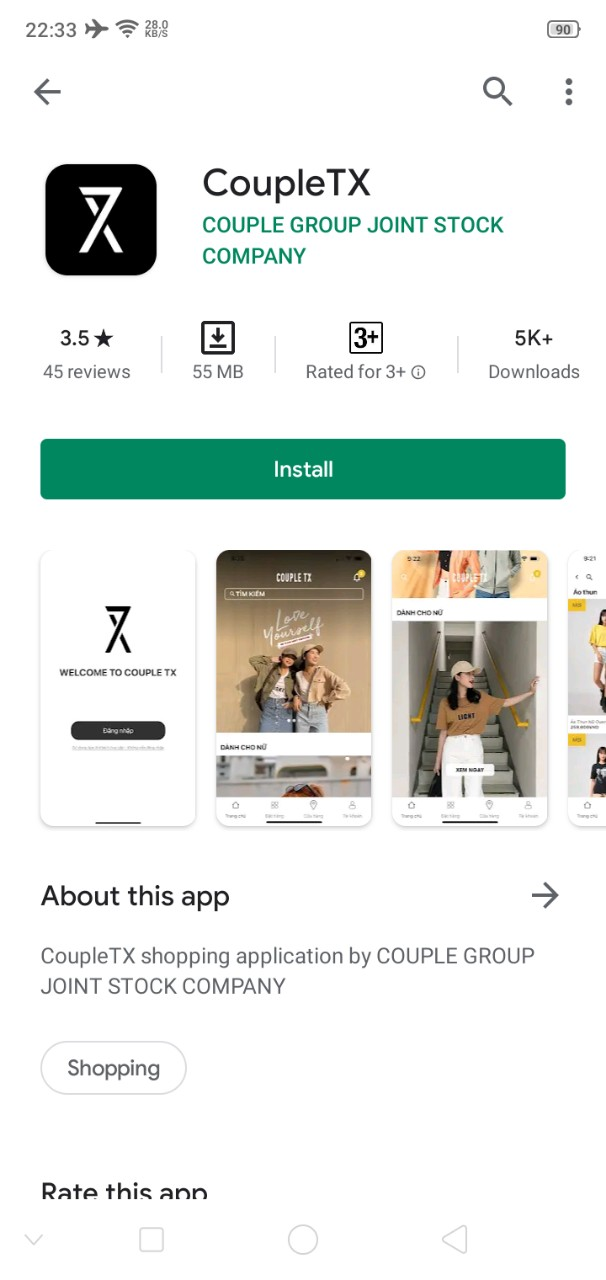
\includegraphics[height=10cm]{images/01.png}
    \caption{Ứng dụng CoupleTX trên GooglePlay}
\end{figure}

\indent và \textbf{Mr.Simple} - thời trang vest, blazer cho nam giới.

\begin{figure}[H]
    \centering
    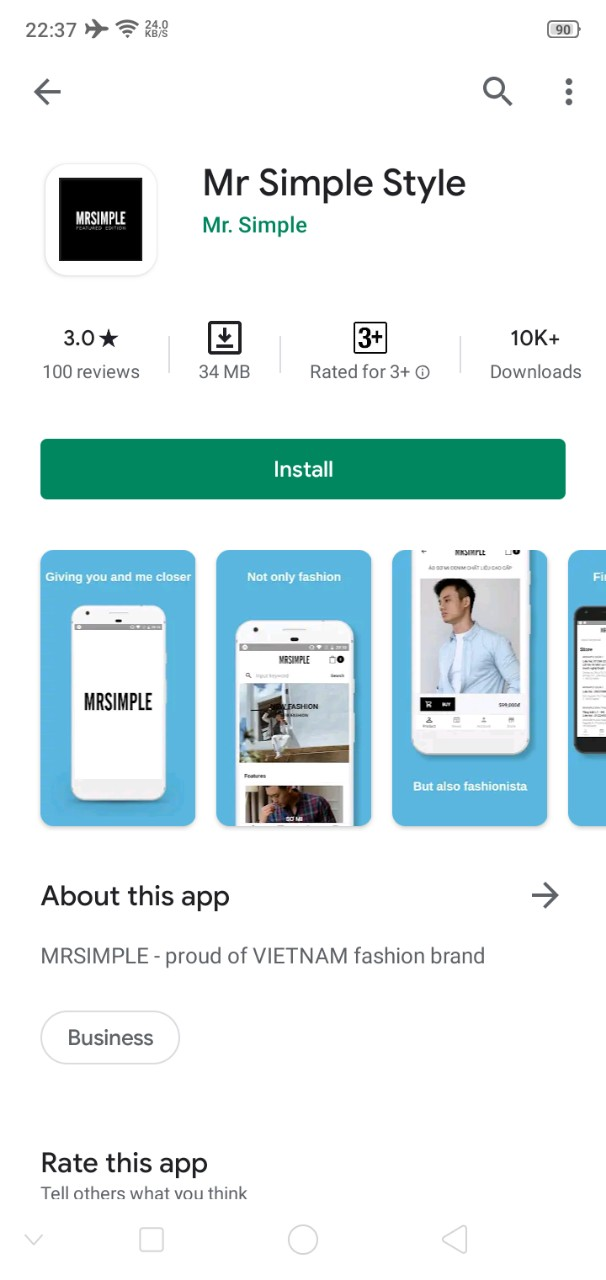
\includegraphics[height=10cm]{images/02.png}
    \caption{Ứng dụng Mr.Simple trên GooglePlay}
\end{figure}

\newpage
\indent Ngoài ra, ngoài phạm vị Việt Nam còn có ứng dụng mua sắm thời trang Farfetch.

\begin{figure}[H]
    \centering
    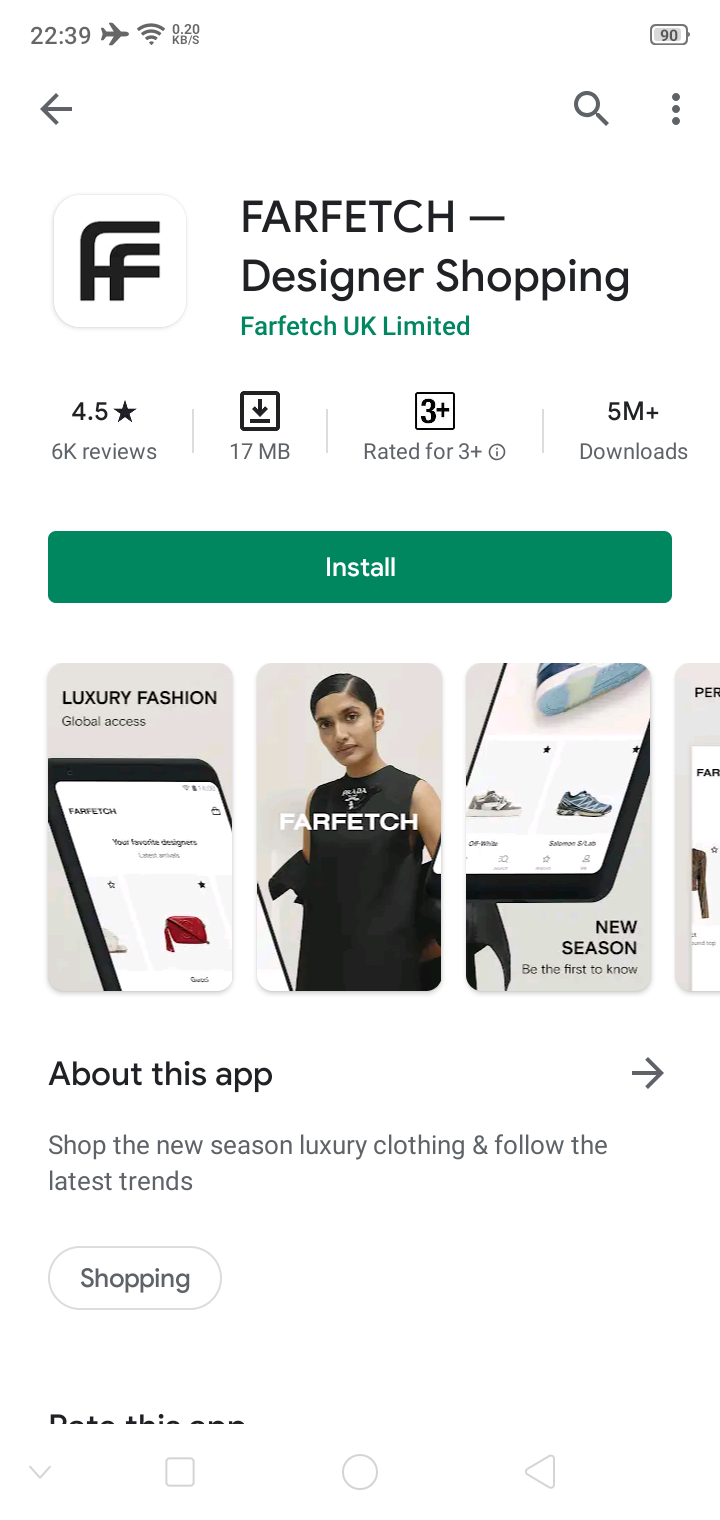
\includegraphics[height=10cm]{images/03.png}
    \caption{Ứng dụng Farfetch trên GooglePlay}
\end{figure}

\subsubsection{Điểm khác biệt của chương trình}
Không có.\\
\indent \textbf{Hạn chế}: Ứng dụng chỉ chạy ở phía client, không có web service nên một vài tính năng dù có trên front-end nhưng bên dưới backend thì chưa hỗ trợ và chưa có server.

\subsection{Đóng góp của các thành viên cho đồ án}
\subsubsection{Tỉ lệ đóng góp của các thành viên}
\begin{tabular}{ |p{1cm}||p{3cm}|p{6cm}|p{5cm}|  }
    \hline
    \textbf{STT} & \textbf{MSSV} & \textbf{Họ và tên}  & \textbf{Đóng góp} (tổng 100\%) \\
    \hline \hline
    1            & 19424915      & Dương Trọng Đức     & 32\%                           \\ \hline
    2            & 20424008      & Dương Mạnh Cường    & 35\%                           \\ \hline
    3            & 20424013      & Phạm Nguyễn Mỹ Diễm & 33\%                           \\
    \hline
\end{tabular}

\subsubsection{Chi tiết các công việc đã thực hiện}
\textbf{Lưu ý:} Các màn hình, tính năng mà nhóm đã đề cập ở báo cáo lần đầu nếu không có trong danh sách dưới đây thì là do nhóm chủ động dừng phát triển do không kiệp tiến độ thời gian môn học, phân bổ thời gian cho các thành viên trong nhóm để làm các đồ án môn học khác. Mong Thầy thông cảm cho nhóm.\\\\

\begin{tabular}{ |p{1cm}||p{3cm}|p{12cm}| }
    \hline
    \textbf{STT} & \textbf{SV thực hiện} & \textbf{Tên chức năng}                                                                                                                                 \\
    \hline \hline
    1            & 19424015              & Đăng ký tài khoản bằng email và password.                                                                                                              \\ \hline
    2            & 19424015              & Đăng nhập tài khoản bằng email và password.                                                                                                            \\ \hline
    3            & 19424015              & Đăng xuất tài khoản người dùng.                                                                                                                        \\ \hline
    4            & 19424015              & Khôi phục mật khẩu cho tài khoản bằng mail gửi đến cho email dùng để đăng ký tài khoản.                                                                \\ \hline
    5            & 19424015              & Màn hình cá nhân người dùng.                                                                                                                           \\ \hline
    6            & 20424008              & Màn hình chính của ứng dụng.                                                                                                                           \\ \hline
    7            & 20424008              & Màn hình splash-screen (trước đây được thực hiện bởi sinh viên 19424015 - sau này do sinh viên 20424008 chỉnh sửa thêm để phục vụ cho màn hình chính). \\ \hline
    8            & 20424008              & Màn hình sản phẩm yêu thích.                                                                                                                           \\ \hline
    9            & 20424008              & Chức năng tìm kiếm.                                                                                                                                    \\ \hline
    10           & 20424013              & Màn hình chi tiết sản phẩm.                                                                                                                            \\ \hline
    11           & 20424013              & Màn hình giỏ hàng.                                                                                                                                     \\ \hline
    12           & 20424013              & Màn hình thanh toán.                                                                                                                                   \\ \hline
    13           & 20424013              & Màn hình lịch sử đơn hàng.                                                                                                                             \\ \hline
\end{tabular}

\subsection{Thông tin cần thiết để chạy chương trình}
\textbf{Đối với ứng dụng sau khi release thành file *.apk}: Chỉ cần tải và cài đặt file \textsf{app-release.apk} trên thiết bị Android chạy Android 9.0 trở lên.\\

\textbf{Đối với giai đoạn phát triển:}
\begin{itemize}
    \item Cần được cấp quyền truy cập vào Firebase console từ trưởng nhóm để chỉnh sửa, thay đổi cài đặt các dịch vụ Firestore, Firestorage và Authentication.
    \item Android Emulator phải chạy Android 9.0 trở lên.
    \item Android Studio phải cài đặt SDK API 28.
\end{itemize}

\section{Các chức năng đã thực hiện}
Phần này sẽ mô tả chi tiết các công việc mà các thành viên của nhóm đã thực hiện trong mục 1.3.2. \textit{(vì để tiện cho việc trình bày, nhóm sẽ không trình bày theo thứ tự như đã liệt kê trong bảng, mong Thầy thông cảm)}.\\

\indent Dưới đây là logo của ứng dụng ở màn hình chính của thiết bị Anroid sau khi cài đặt \textit{(chú ý mũi tên màu đỏ)}.

\begin{figure}[H]
    \centering
    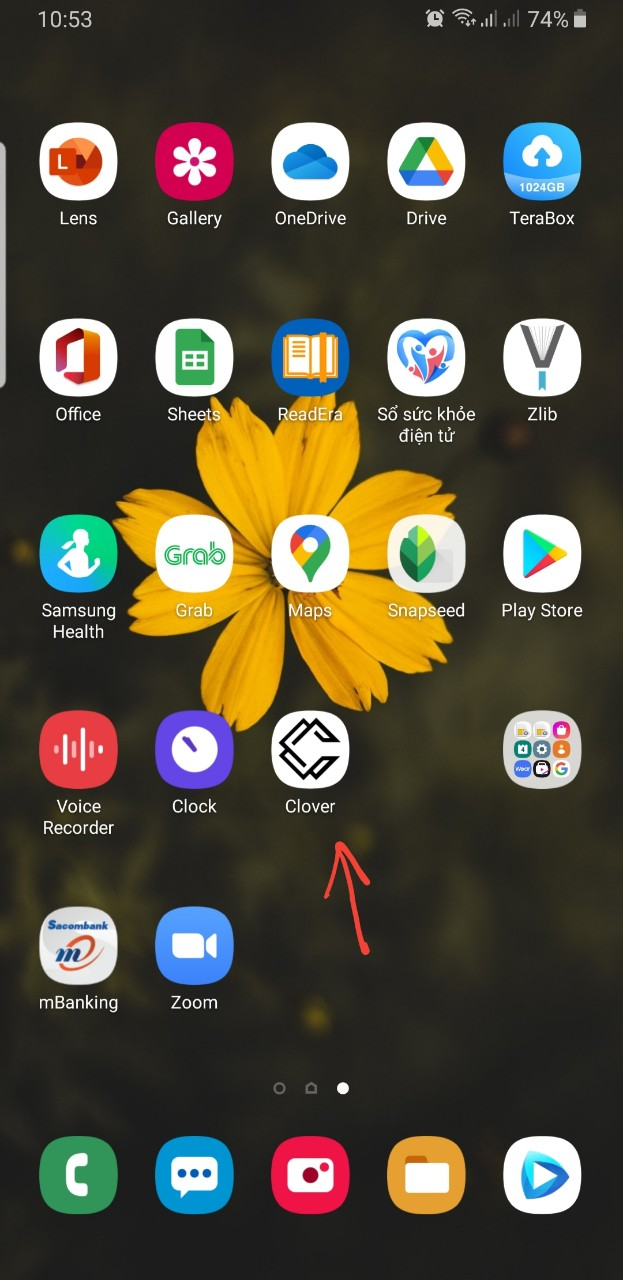
\includegraphics[height=10cm]{images/04.png}
    \caption{Logo của ứng dụng ở màn hình menu của thiết bị Android}
\end{figure}

\newpage
\subsection{Màn hình splash-screen}
Được thực hiện bởi sinh viên 20424008. Dưới đây là hình chụp của màn hình này.

\begin{figure}[H]
    \centering
    
\includegraphics[height=10cm]{images/05.png}
    \caption{Màn hình splash-screen}
\end{figure}

\indent Khi truy cập vào ứng dụng, người dùng sẽ gặp màn hình này đầu tiên.\\\\
\indent \textbf{Các thành phần và chức năng kèm theo trên màn hình}
\begin{itemize}
    \item Màn hình này sẽ hiển thị trong ba giây.
    \item Trong ba giây, back-end sẽ load dữ liệu như hình ảnh, tên sản phẩm, các custom icon của ứng dụng... từ Firestore về thiết bị để giảm tải cho màn hình chính. Người dùng cũng tránh việc có "cảm giác" phải chờ đợi.
    \item Kiểm tra người dùng là người dùng mới hay là người dùng cũ.
    
    \begin{itemize}
        \item Nếu là người dùng cũ thì sẽ đi thẳng đến màn hình chính của ứng dụng.
        \item Nếu là người dùng mới (người dùng cũ nhưng đã đăng xuất tài khoản, người dùng vừa cài ứng dụng lên thiết bị,...) thì sẽ đi thẳng đến màn hình đăng nhập.
    \end{itemize}
\end{itemize}

\subsection{Màn hình đăng nhập}
\subsubsection{Chức năng đăng nhập}
Được thực hiện bởi sinh viên 19424015. Dưới đây là hình chụp của màn hình này.\\

\indent Chức năng đăng nhập này sử dụng dịch vụ Firebase Authentication của Google cung cấp.\\

\indent Người dùng sẽ được đưa đến màn hình này khi:
\begin{itemize}
    \item Là người dùng cũ nhưng đã đăng xuất tài khoản.
    \item Là người dùng mới (vừa cài đặt ứng dụng).
    \item Người dùng bỏ qua bước đăng nhập đi thẳng vào màn hình chính nhưng về sau lại có nhu cầu đăng nhập để đặt hàng, thanh toán,... và được màn hình chính đưa lại về đây. 
\end{itemize}

\begin{figure}[H]
    \centering
    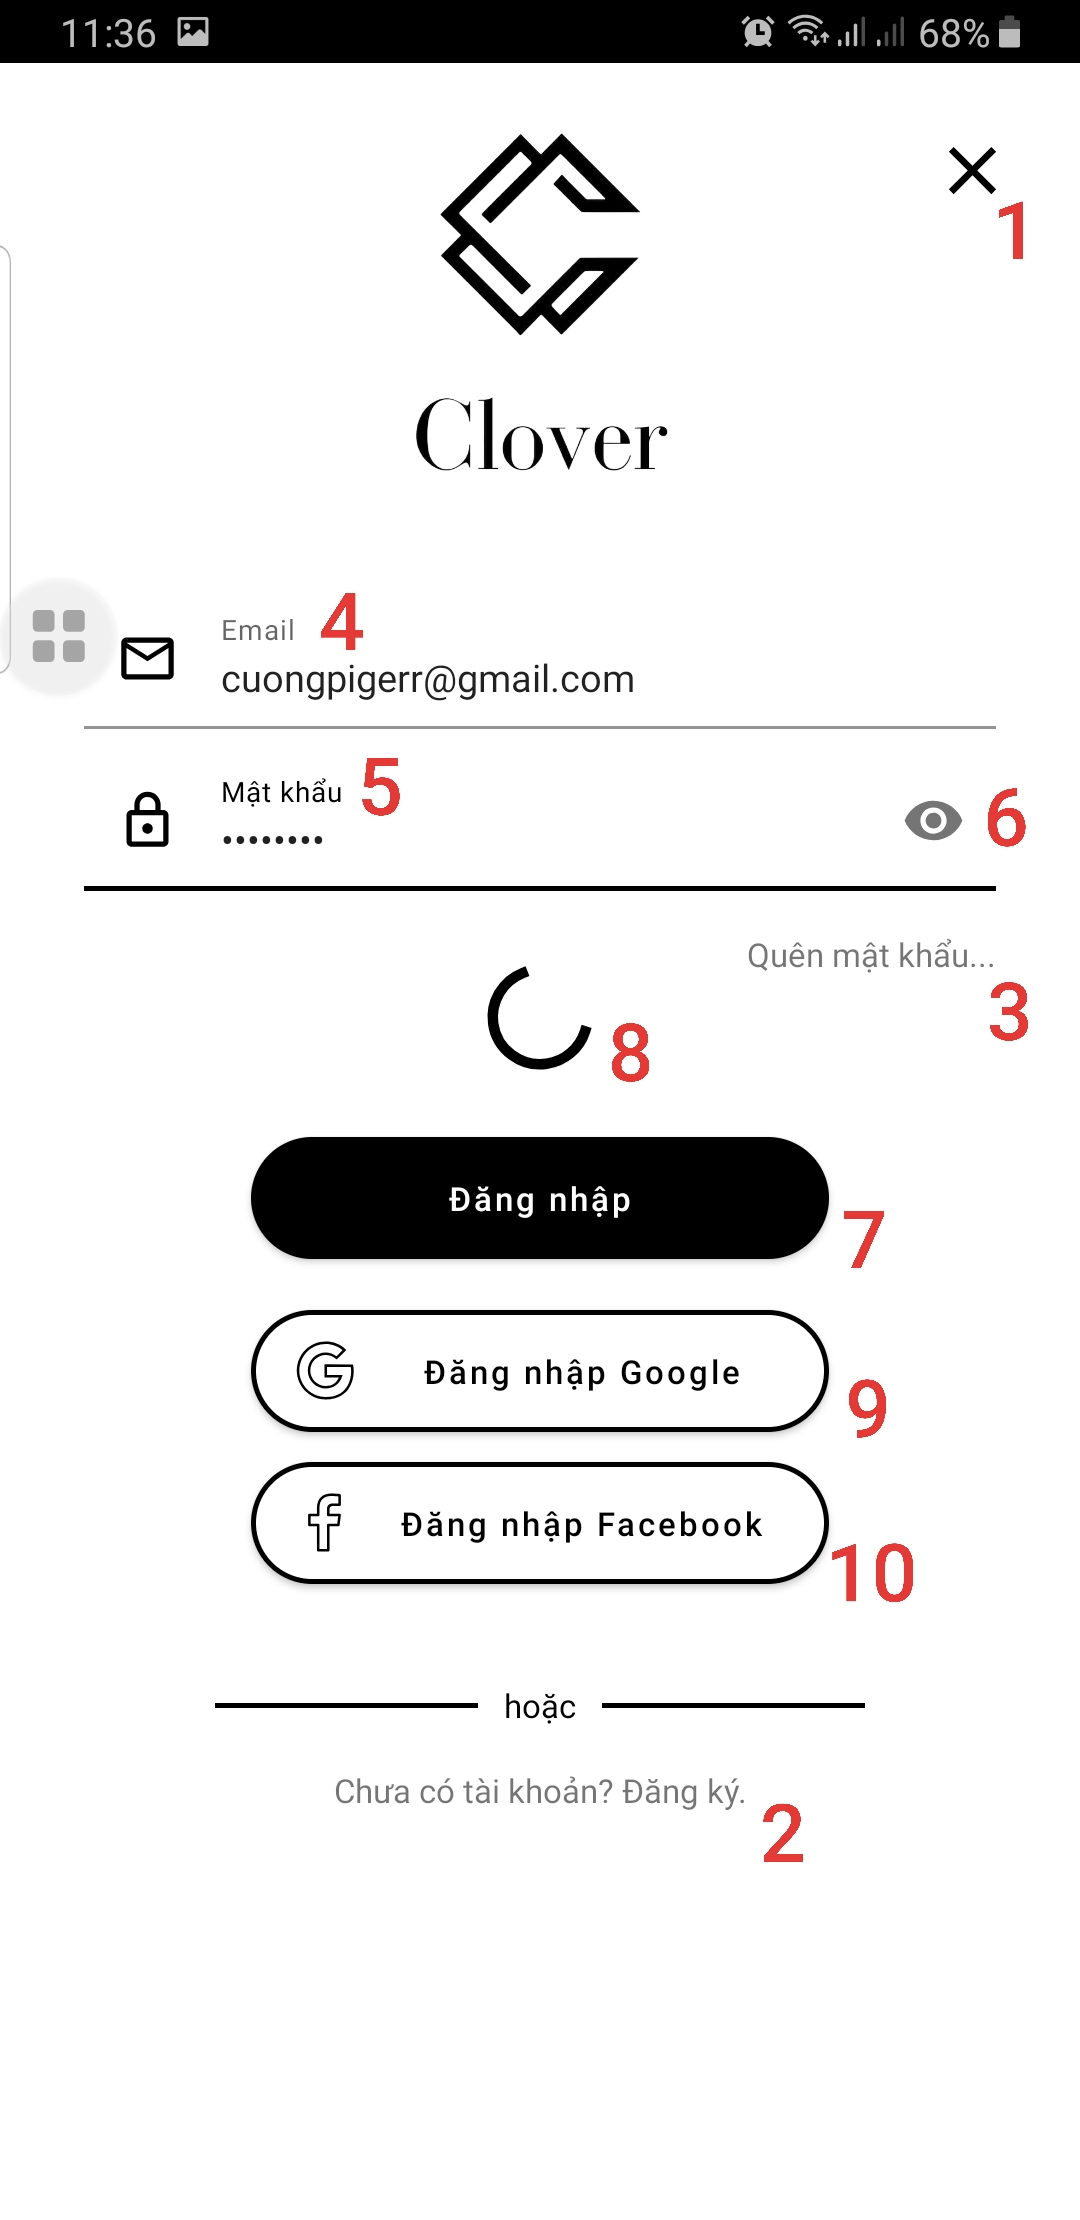
\includegraphics[height=10cm]{images/06.png}
    \caption{Màn hình đăng nhập - chức năng đăng nhập}
\end{figure}

\indent \textbf{Các thành phần và chức năng kèm theo trên màn hình}
\begin{itemize}
    \item \textbf{1}: Image button - khi nhấn vào button này người dùng sẽ được chuyển thẳng đến màn hình chính của ứng dụng mà \textbf{không cần đăng nhập}.
    \item \textbf{2}: Text button - khi nhấn vào sẽ đưa đến fragment đăng ký tài khoản mới cho người dùng ở mục 2.2.3.
    \item \textbf{3}: Text button - khi nhấn vào đưa người dùng đến fragment đặt lại mật khẩu ở mục 2.2.2.
    \item \textbf{4}: Text input layout: nhập thông tin email của người dùng. Trong quá trình người dùng typing - thực hiện kiểm tra hợp lệ để thông báo ngay cho người dùng biết.
    \item \textbf{5}: Text input layout: nhập mật khẩu của người dùng.
    \item \textbf{6}: Icon - Khi nhấn vào sẽ hiển thị mật khẩu ở \textbf{5} ra dưới dạng text.
    \newpage
    \item \textbf{7}: Button - khi nhấn vào sẽ lấy thông tin ở \textbf{4} và \textbf{5} $\Rightarrow$  kiểm tra hợp lệ (nếu không hợp lệ sẽ thông báo ngay trên Text input layout của \textbf{4} và \textbf{5}) $\Rightarrow$ nếu hợp lệ, đăng nhập vào ứng dụng thông qua Firebase Authentication, sau đó sẽ bị deactive cho đến khi Firebase Authentication xử lý xong.
    \begin{itemize}
        \item \textbf{Nếu thành công}: Người dùng được chuyển thẳng đến màn hình chính của ứng dụng.
        \item \textbf{Nếu thất bại}: Hiển thị một Alert Dialog thông báo cho người dùng biết là đăng nhập thất bại.
    \end{itemize}
    \item \textbf{8}: Progress Circle - luôn ẩn đi, chỉ hiển thị khi người dùng nhấn vào \textbf{7} để cho người dùng biết rằng hệ thống vẫn chạy và đang trong quá trình kiểm tra đăng nhập.
    \item \textbf{9}: Button - dùng để đăng nhập qua Google nhưng chỉ mới có ở front-end, back-end vẫn chưa thực hiện do không kịp tiến độ môn học.
    \item \textbf{10}: Button - dùng để đăng nhập qua Facebook nhưng chỉ mới có ở front-end, back-end vẫn chưa thực hiện do không kịp tiến độ môn học.
\end{itemize}

\subsubsection{Chức năng đặt lại mật khẩu}
Được thực hiện bởi sinh viên 19424015. Dưới đây là hình chụp của màn hình này.\\

\indent Chức năng đặt lại mật khẩu sử dụng Firebase Authentication để gửi mail kèm theo link đặt lại password về cho email mà người dùng dùng để đăng nhập tài khoản.\\

\indent Người dùng sẽ được đưa về fragment này sau khi nhấn vào thành phần \textbf{3} trên fragment đăng nhập ở mục 2.2.1.

\begin{figure}[H]
    \centering
    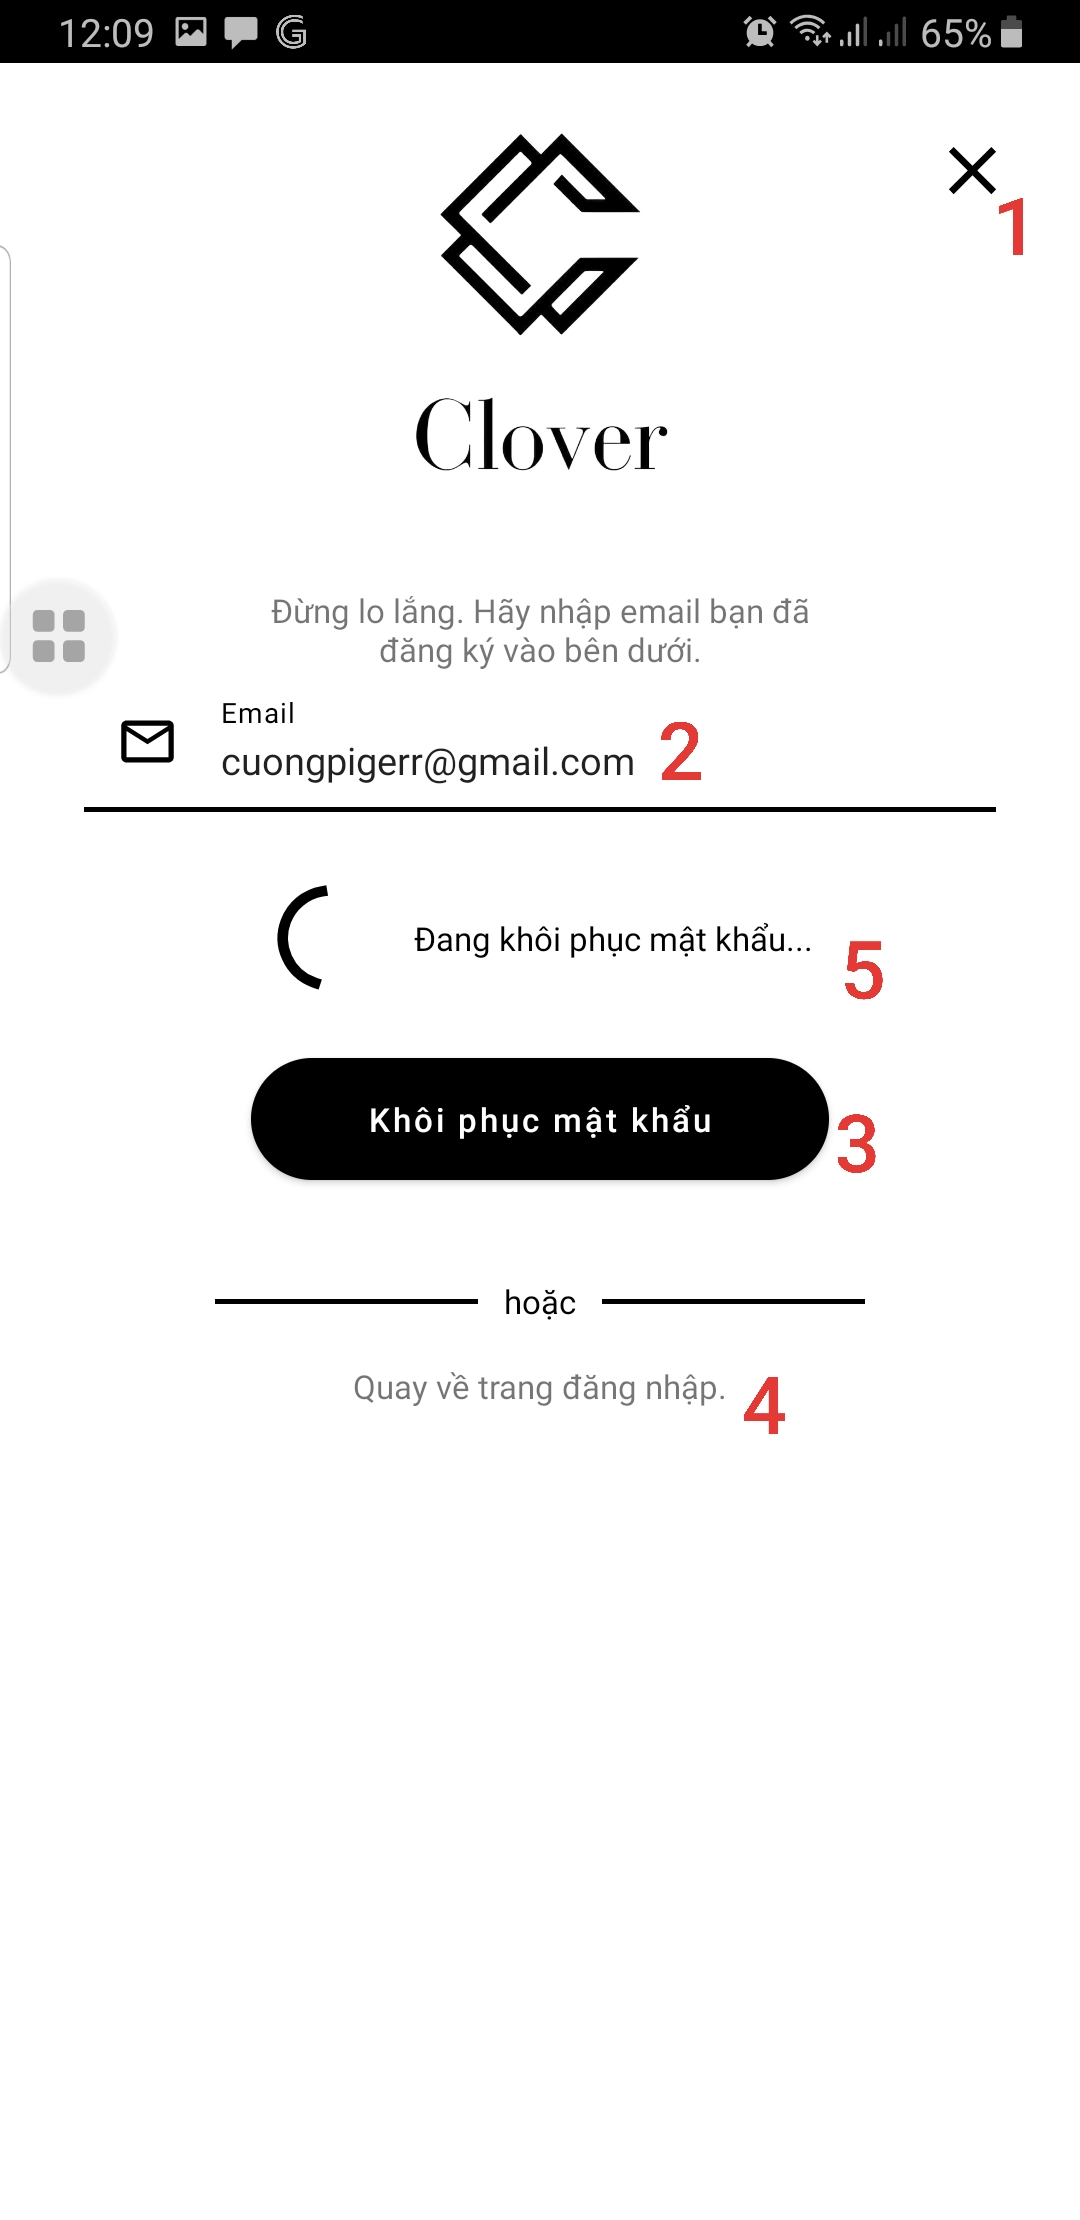
\includegraphics[height=10cm]{images/07.png}
    \caption{Màn hình đặt lại mật khẩu - nhập thông tin}
\end{figure}

\begin{figure}[H]
    \centering
    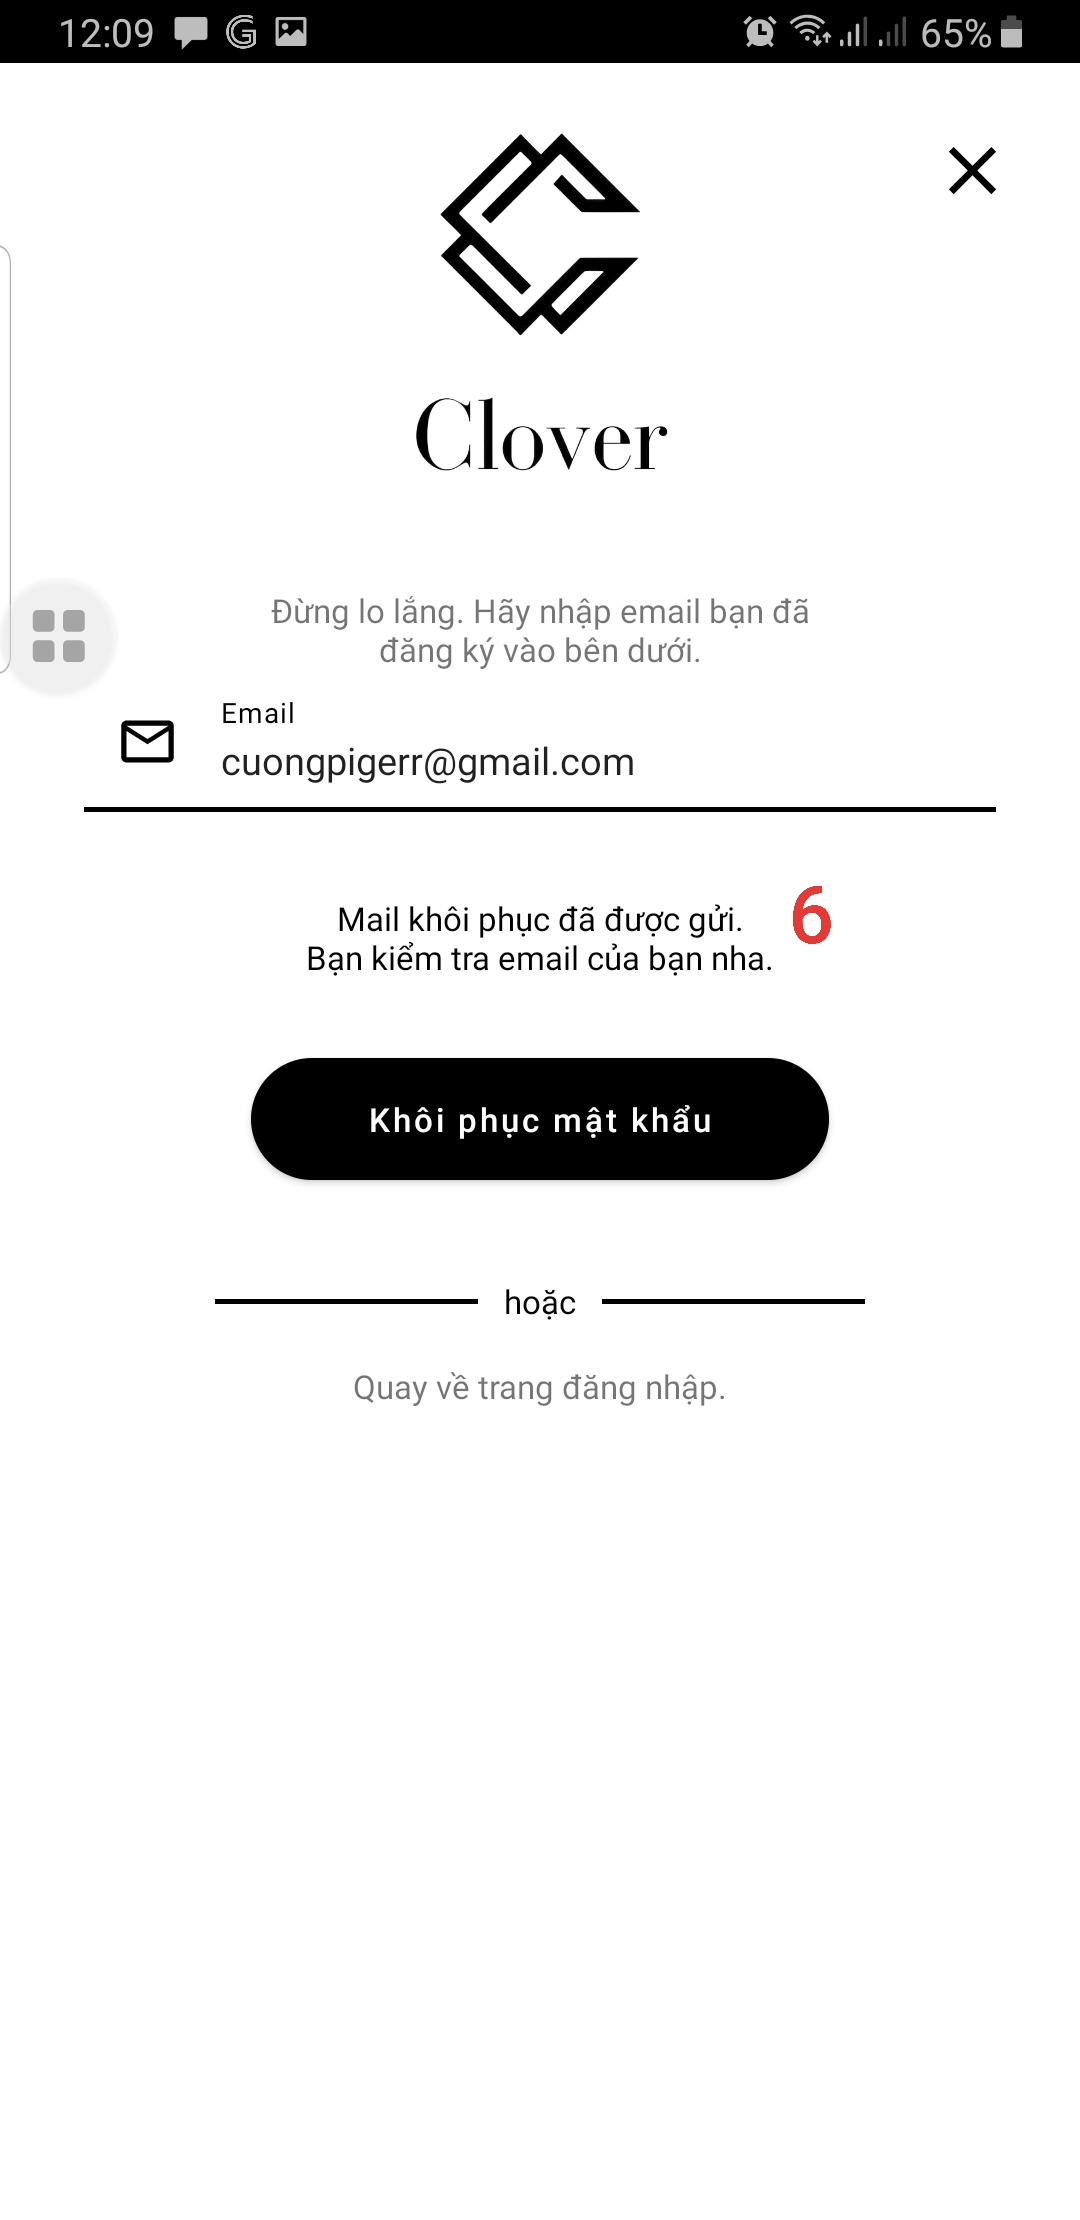
\includegraphics[height=10cm]{images/08.png}
    \caption{Màn hình đặt lại mật khẩu - thông báo cho người dùng biết đã gửi mail thành công}
\end{figure}

\begin{figure}[H]
    \centering
    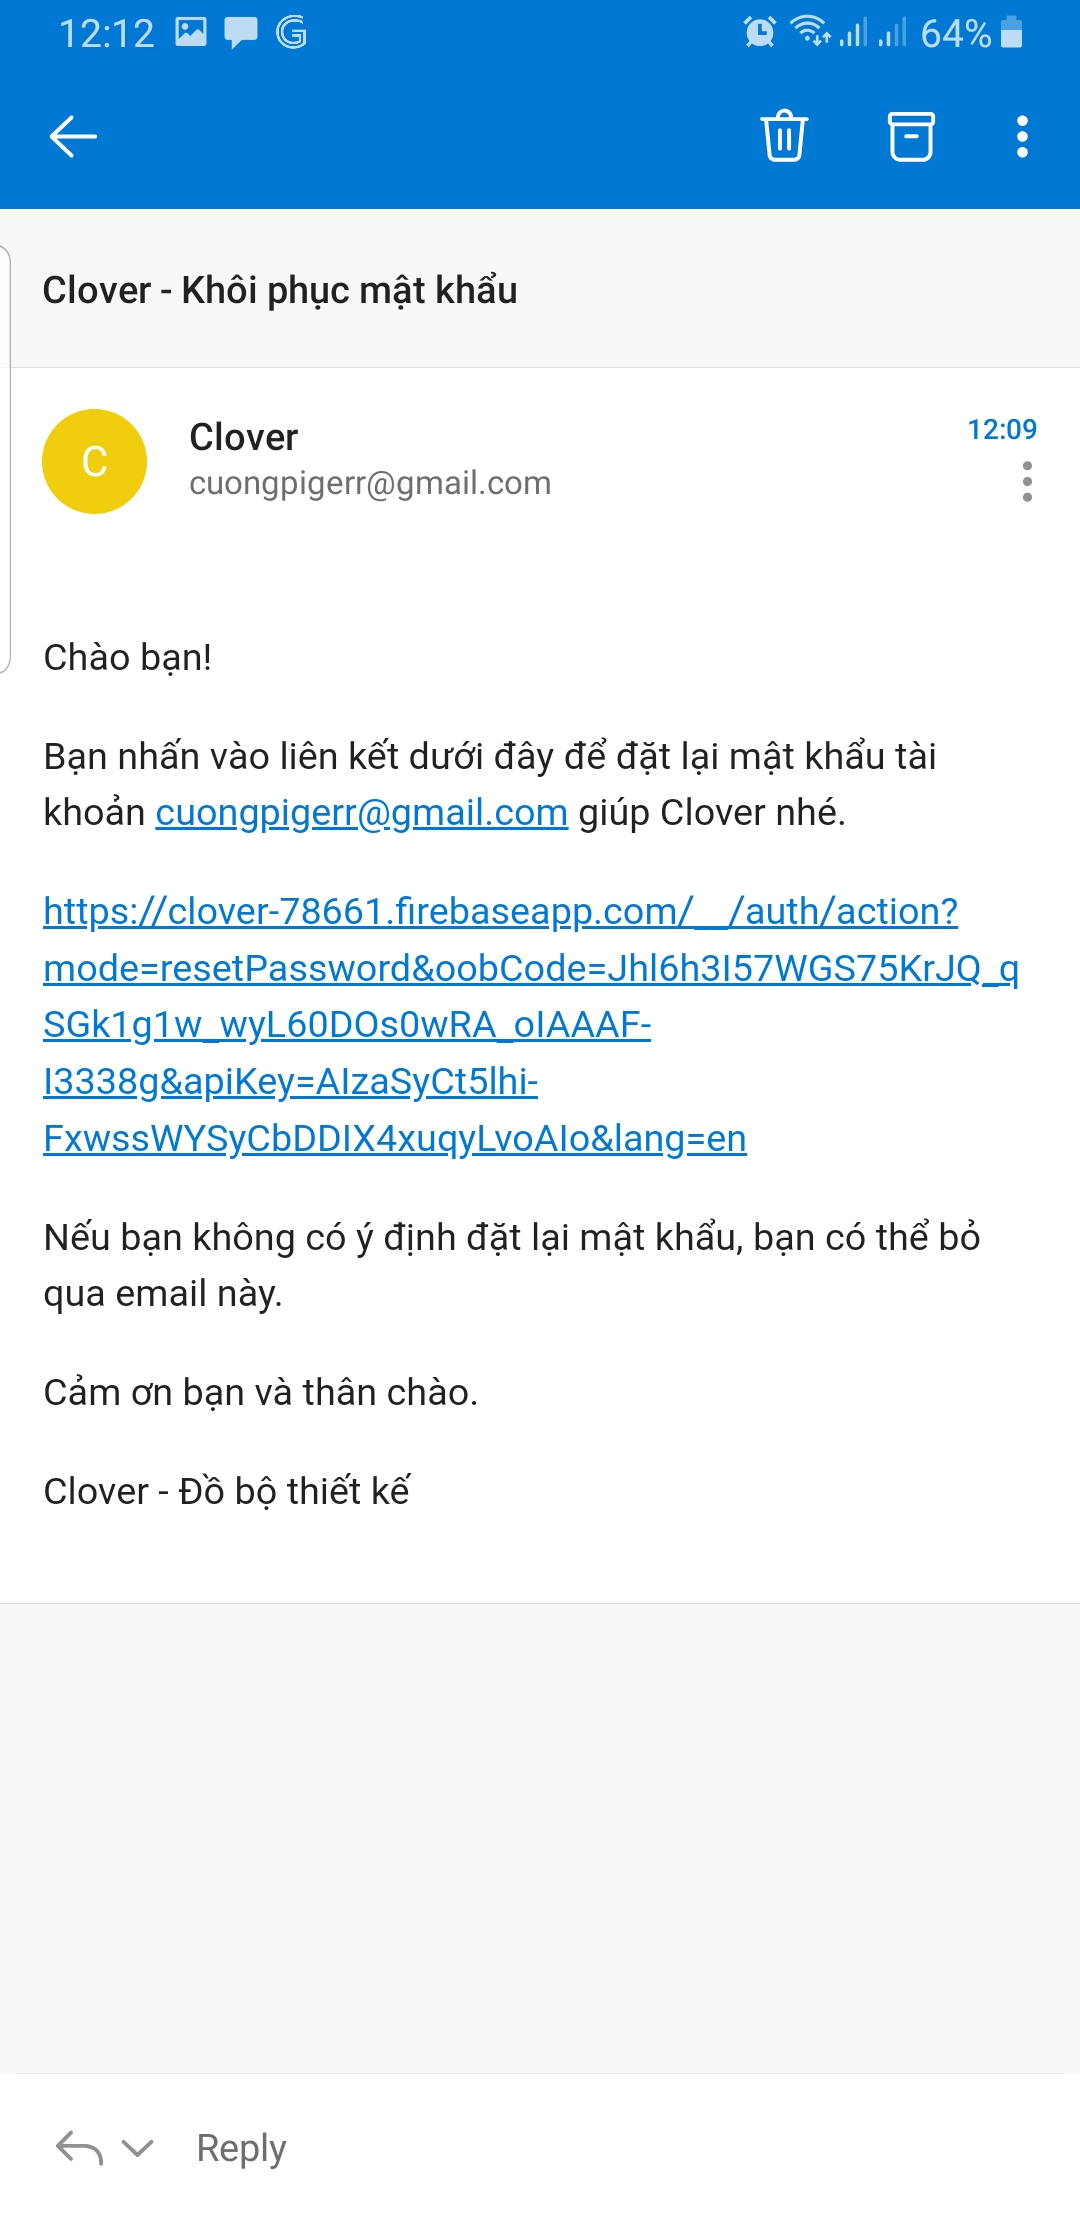
\includegraphics[height=10cm]{images/09.png}
    \caption{Mail khôi phục kèm link đặt lại mật khẩu được gửi về cho email mà người dùng dùng để đăng nhập tài khoản}
\end{figure}

\indent \textbf{Các thành phần và chức năng kèm theo trên màn hình}
\begin{itemize}
    \item \textbf{1}: Image button - nhấn vào để đi thẳng đến màn hình chính của ứng dụng mà không cần đăng nhập.
    \item \textbf{2}: Text input layout - nhập email mà người dùng muốn đặt lại mật khẩu.
    \item \textbf{3}: Button - nhấn vào để gửi mail đặt lại mật khẩu.
    \item \textbf{4}: Text button - nhấn vào để trở về chức năng đăng nhập ở mục 2.2.1.
    \item \textbf{5}: Progress circle + Text view: cho người dùng biết mail khôi phục mật khẩu đang được gửi đến email được cung cấp ở \textbf{2}.
    \item \textbf{6}: Text view - cho người dùng biết đã gửi mail thành công.
\end{itemize}

\subsubsection{Chức năng đăng ký tài khoản}
Được thực hiện bởi sinh viên 19424015. Dưới đây là hình chụp của màn hình này.\\

\indent Chức năng đăng ký tài khoản sử dụng Firebase Authentication để đăng ký tài khoản cho người dùng.\\

\indent Người dùng sẽ được đưa thẳng đến fragment này sau khi nhấn vào thành phần \textbf{2} trên fragment đăng nhập ở mục 2.2.1.

\begin{figure}[H]
    \centering
    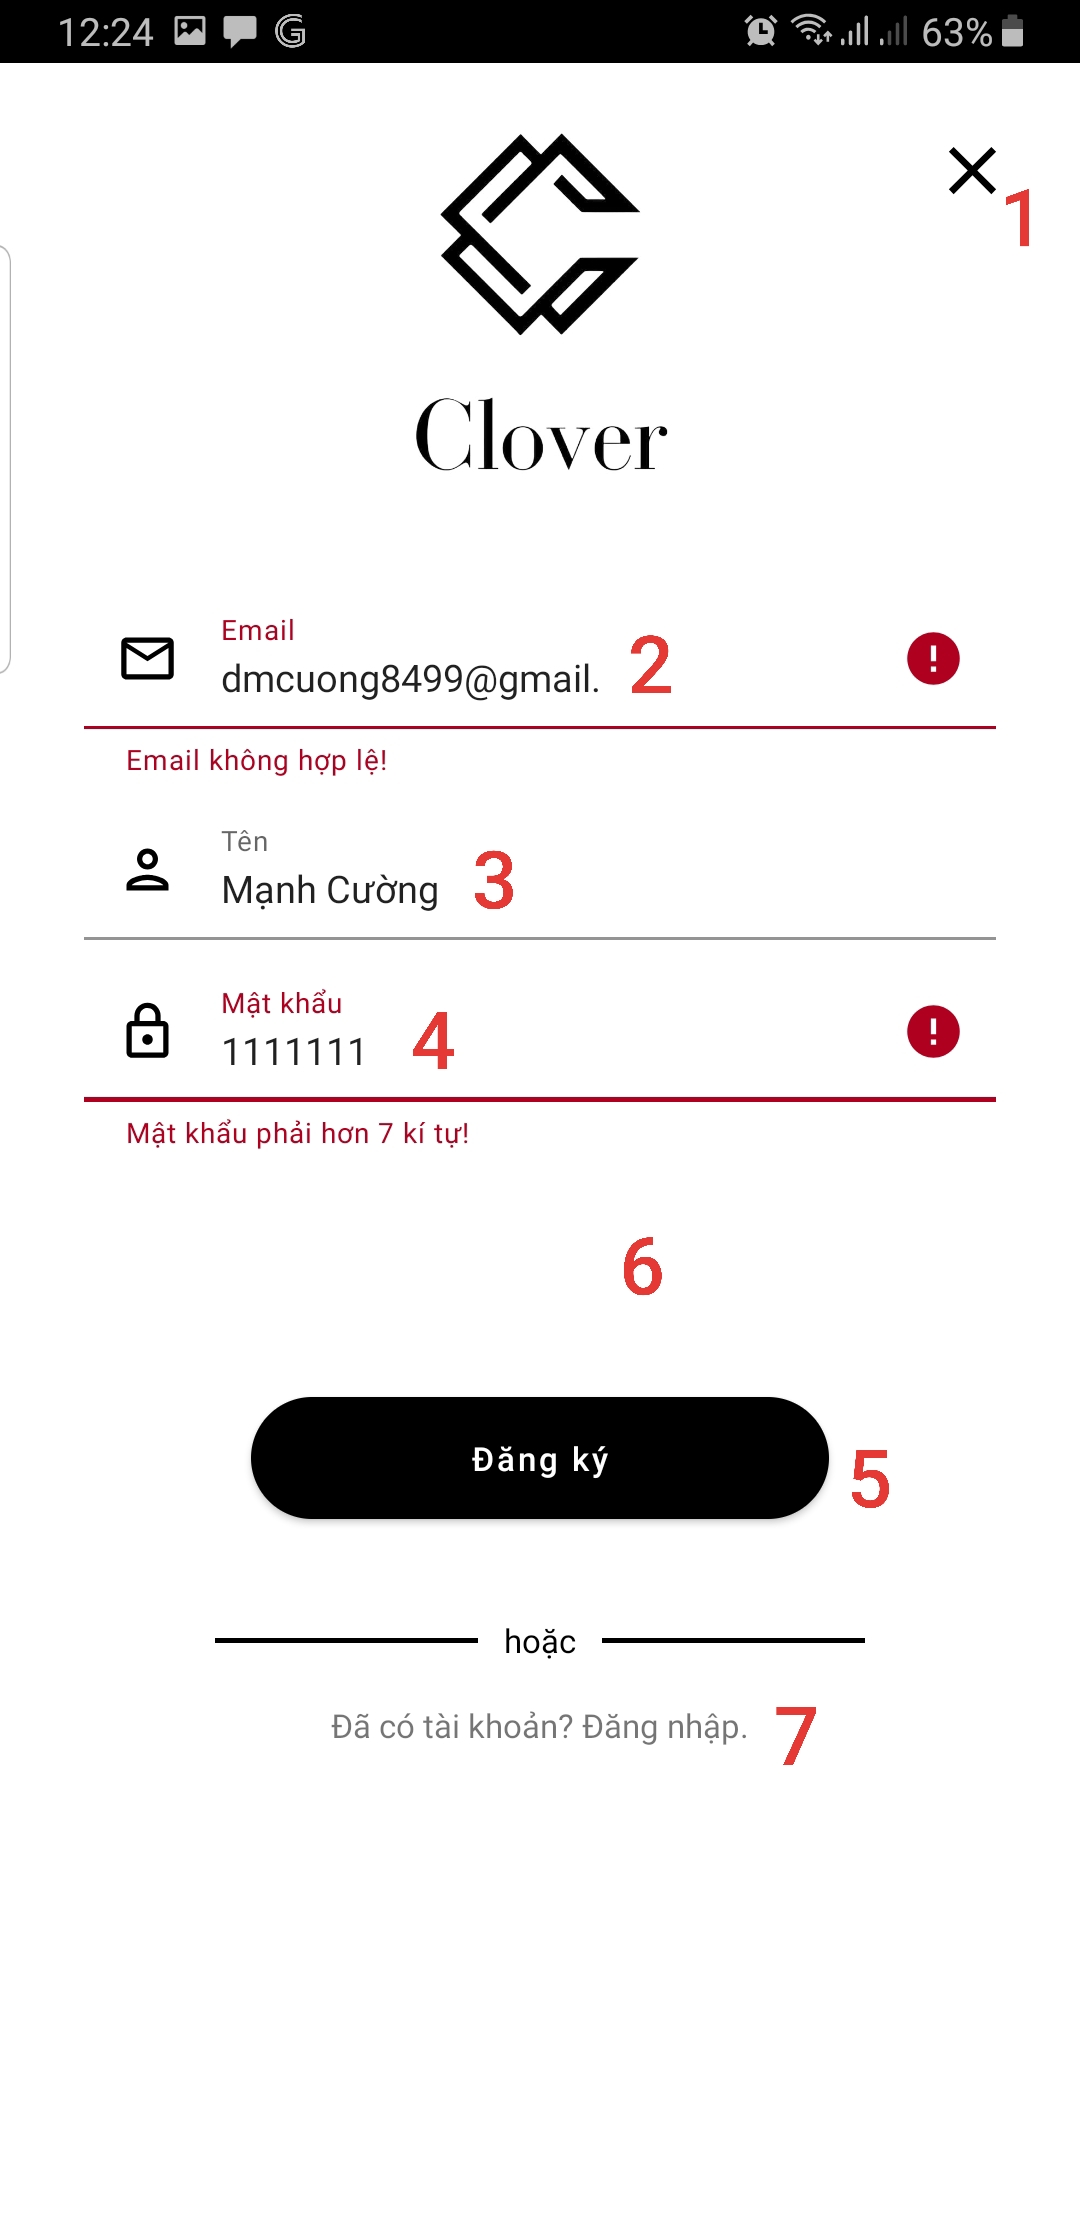
\includegraphics[height=10cm]{images/10.png}
    \caption{Màn hình đăng ký tài khoản}
\end{figure}

\indent \textbf{Các thành phần và chức năng kèm theo trên màn hình}
\begin{itemize}
    \item \textbf{1}: Image button - nhấn vào để đi thẳng đến màn hình chính của ứng dụng mà không cần đăng nhập.
    \item \textbf{2}: Text input layout - nhập email mà người dùng muốn tạo tài khoản (ở đây nhóm cố tình nhập sai định dạng email để Thầy có thể thấy được là ứng dụng có kiểm tra hợp lệ của các trường dữ liệu).
    \item \textbf{3}: Text input layout - nhập tên cho người dùng.
    \item \textbf{4}: Text input layout - nhập mật khẩu cho người dùng (ở đây nhóm cố tình nhập nhập password không hợp lệ để Thầy có thể thấy được là ứng dụng có kiểm tra hợp lệ của các trường dữ liệu).
    \item \textbf{5}: Button - khi nhấn vào, ứng dụng có hai khả năng trả về:
    \begin{itemize}
        \item \textbf{Thành công}: người dùng được đưa thẳng đến màn hình chính của ứng dụng và được Firestore ghi lại các thông tin của người dùng thành một document bên trong collection \textsf{UserModel} (nhóm sẽ trình bày sau).
        \item \textbf{Thất bại}: do email này đã được đăng ký trước đó hoặc vì một nguyên nhân nào đó $\Rightarrow$ hiển thị AlertDialog thông báo cho người dùng biết đăng ký thất bại.
    \end{itemize}

    \newpage
    \item \textbf{6}: Progress circle - về hình ảnh như các progress circle ở fragment đăng nhập + fragment đặt lại mật khẩu và luôn ẩn đi, chỉ hiển thị khi người dùng nhấn vào \textbf{5} (ở đây không hiển thị là do em chưa nhấn vào thành phần \textbf{5} và cũng không thể nhấn vào do \textbf{2} + \textbf{4} vi phạm trường dữ liệu).
    \item \textbf{7}: Image button - nhấn vào sẽ dược chuyển về chức năng đăng nhập ở mục 2.2.1.
\end{itemize}

\subsection{Màn hình chính}
Được thực hiện bởi sinh viên 20424008.\\

\indent Màn hình này được đưa đến khi:
\begin{itemize}
    \item Người dùng nhấn vào thành phần \textbf{1} ở các mục 2.2.1, 2.2.2 và 2.2.3.
    \item Người dùng đăng nhập thành công ở mục 2.2.1.
    \item Người dùng đăng ký tài khoản thành công ở mục 2.2.3.
\end{itemize}

\subsubsection{Màn hình trang chủ}
Được thực hiện bởi sinh viên 20424008. Dưới đây là hình chụp của màn hình này.\\

\begin{figure}[H]
    \centering
    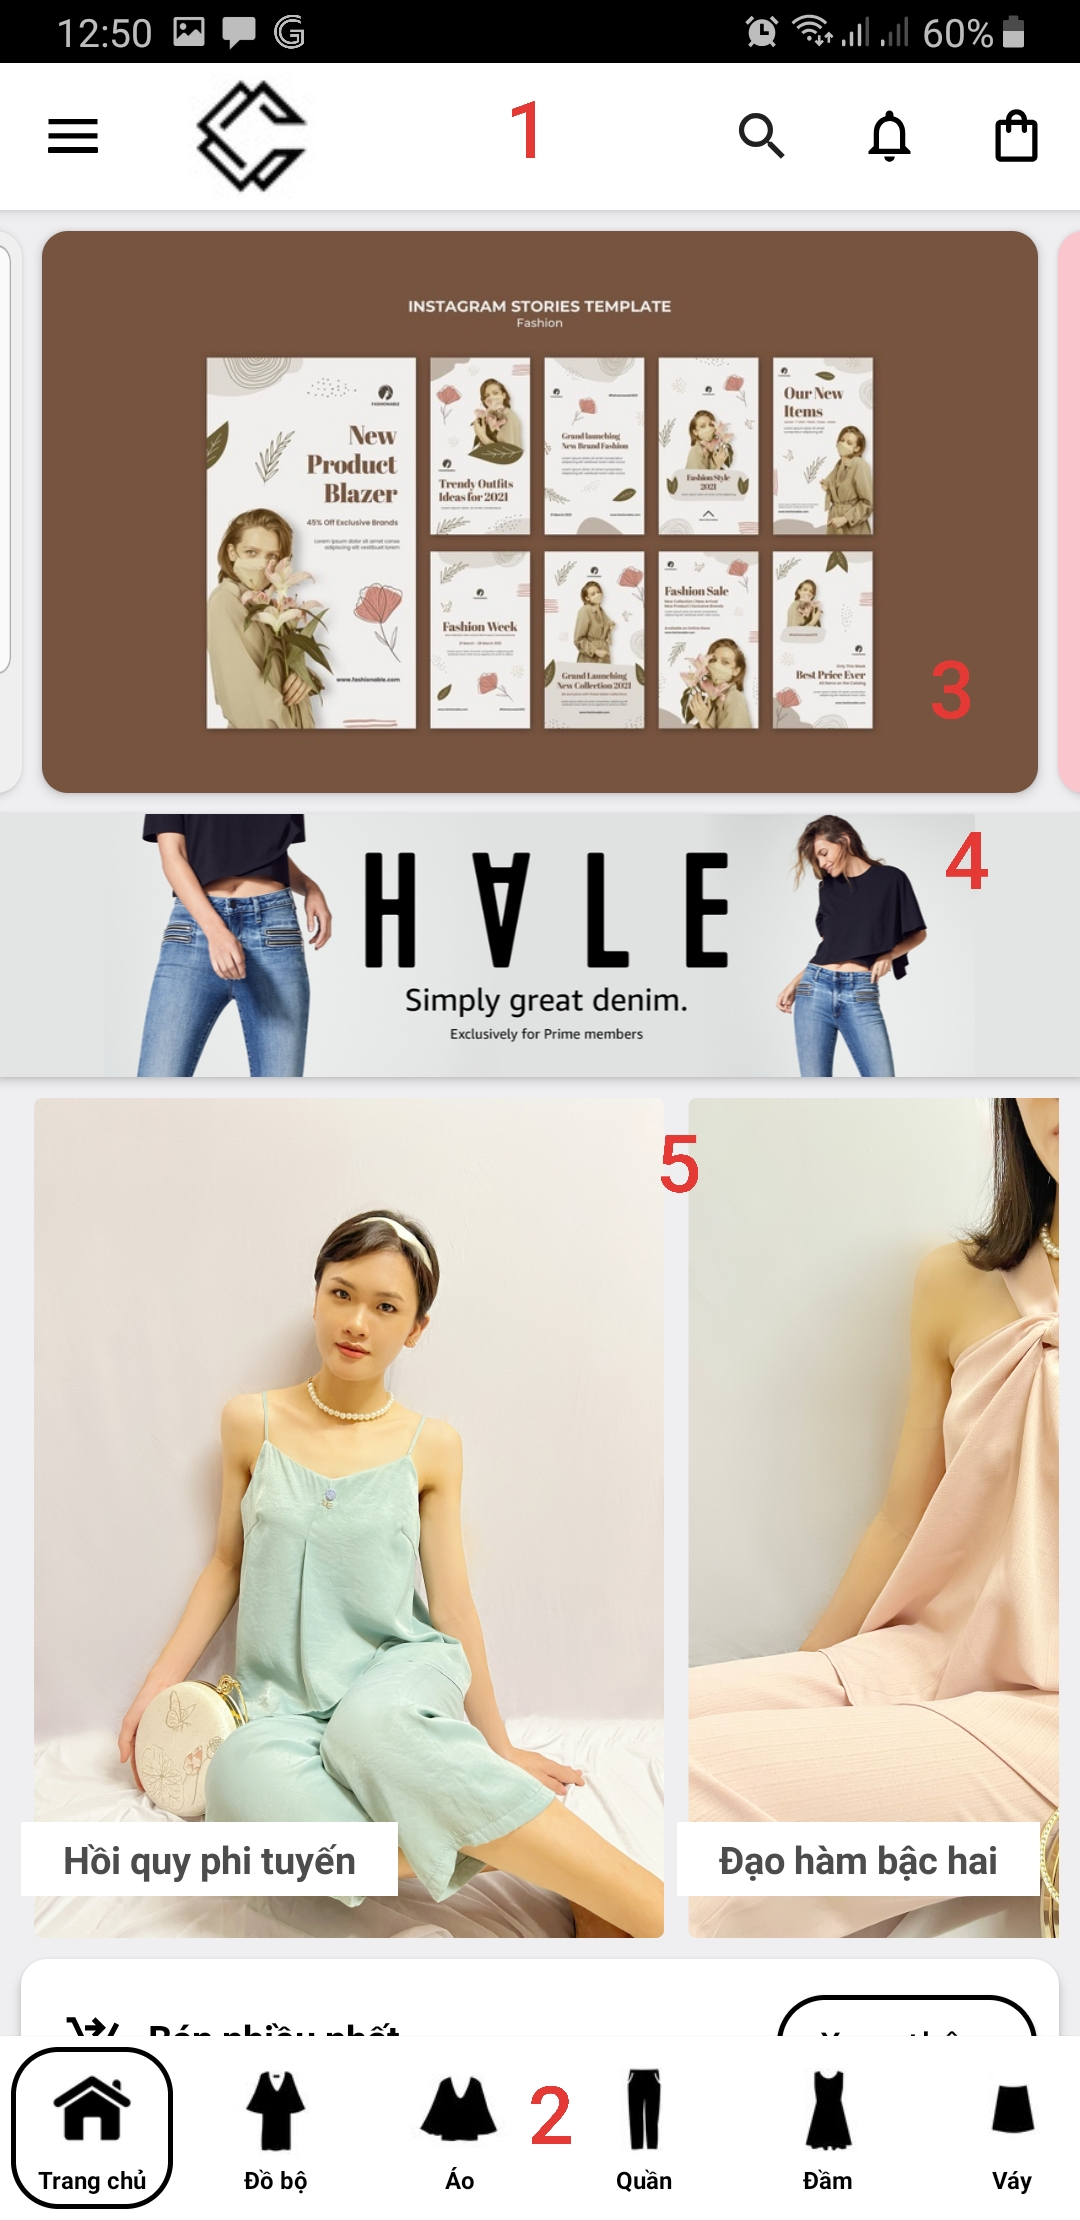
\includegraphics[height=10cm]{images/11.png}
    \caption{Màn hình trang chủ 1}
\end{figure}

\newpage
\indent \textbf{Các thành phần và chức năng kèm theo trên màn hình (1)}
\begin{itemize}
    \item \textbf{1}: Action bar - chứa các thành phần từ trái qua phải như sau:
    \begin{itemize}
        \item Hamburger toggle - nhấn vào để mở navigation view.
        \item Actionbar logo - hiển thị logo của ứng dụng.
        \item Menu item Search - chức năng tìm kiếm.
        \item Menu item Notification - chức năng thông báo (chưa hỗ trợ do ứng dụng chưa có web service + server xử lí).
        \item Menu item Cart - bấm vào để đi đến fragment giỏ hàng.
    \end{itemize}

    \item \textbf{2}: Horizontal Recycler View - hiển thị các sản phẩm theo danh mục.
    \item \textbf{3}: Carousel (Horizontal Recycler View) - hiển thị các chương trình, khuyến mãi của cửa hàng. Sau ba giây sẽ tự chuyển.
    \item \textbf{4}: Banner (Image View) - dùng để chèn quảng cáo.
    \item \textbf{5}: Slider (Horizontal Recycler View) - hiển thị các sản phẩm mới nhất. Nhấn vào item sẽ đưa đến trang chi tiết sản phẩm tương ứng, fragment này được trình bày trong mục 2.3.4.
\end{itemize}

\newpage
\begin{figure}[H]
    \centering
    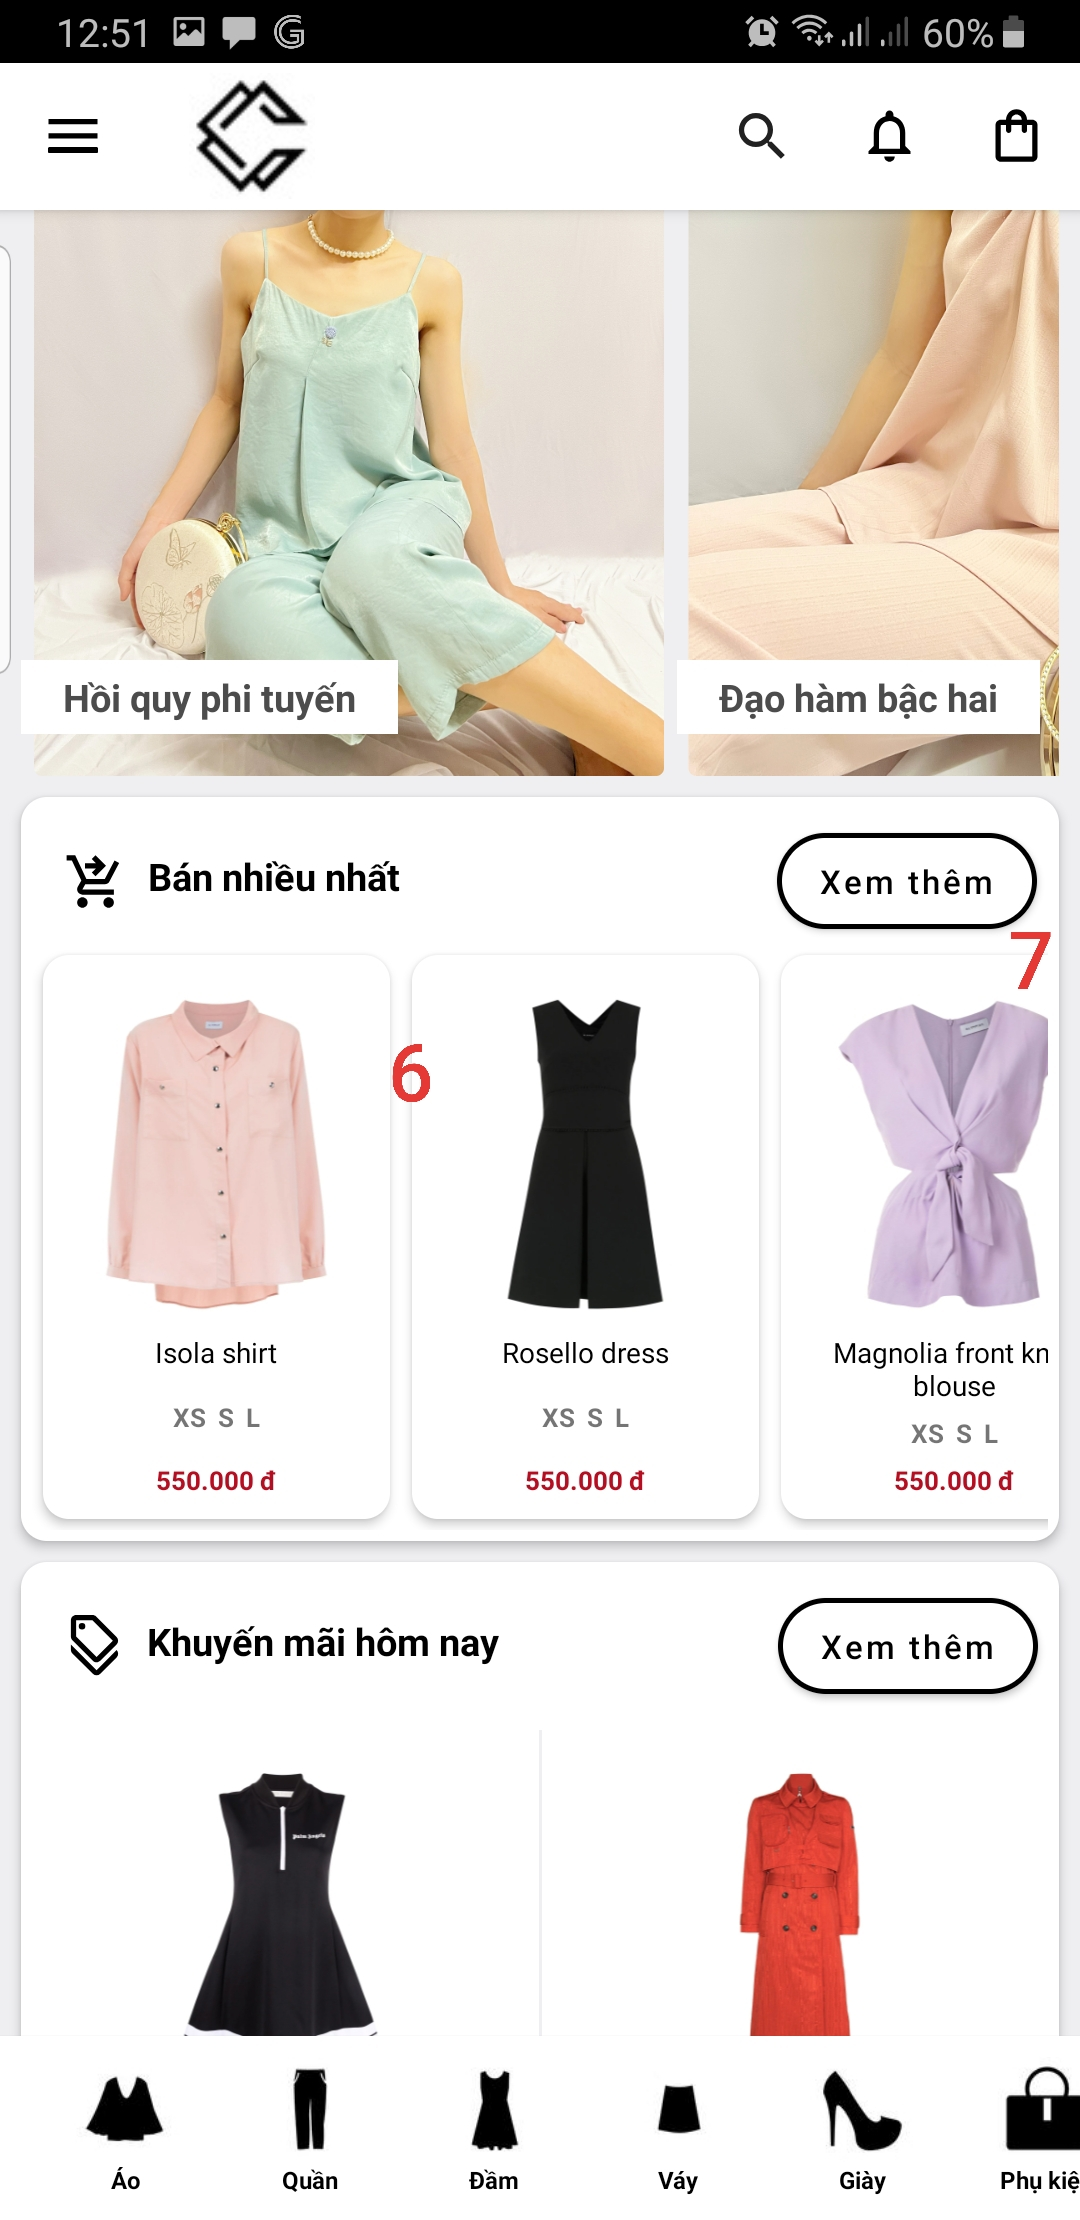
\includegraphics[height=10cm]{images/12.png}
    \caption{Màn hình trang chủ 2}
\end{figure}

\indent \textbf{Các thành phần và chức năng kèm theo trên màn hình (2)}
\begin{itemize}
    \item \textbf{6}: Horizontal Recycler View - hiển thị tám các sản phẩm bán chạy hiện tại. Nhấn vào item sẽ đưa đến trang chi tiết sản phẩm tương ứng, fragment này sẽ trình bày trong mục 2.3.4.
    \item \textbf{7}: Button - đưa đến một fragment khác hiển thị nhiều hơn tám sản phẩm bán chạy dưới dạng GridView, fragment này sẽ được trình bày ở mục 2.3.2.
\end{itemize}

\newpage
\begin{figure}[H]
    \centering
    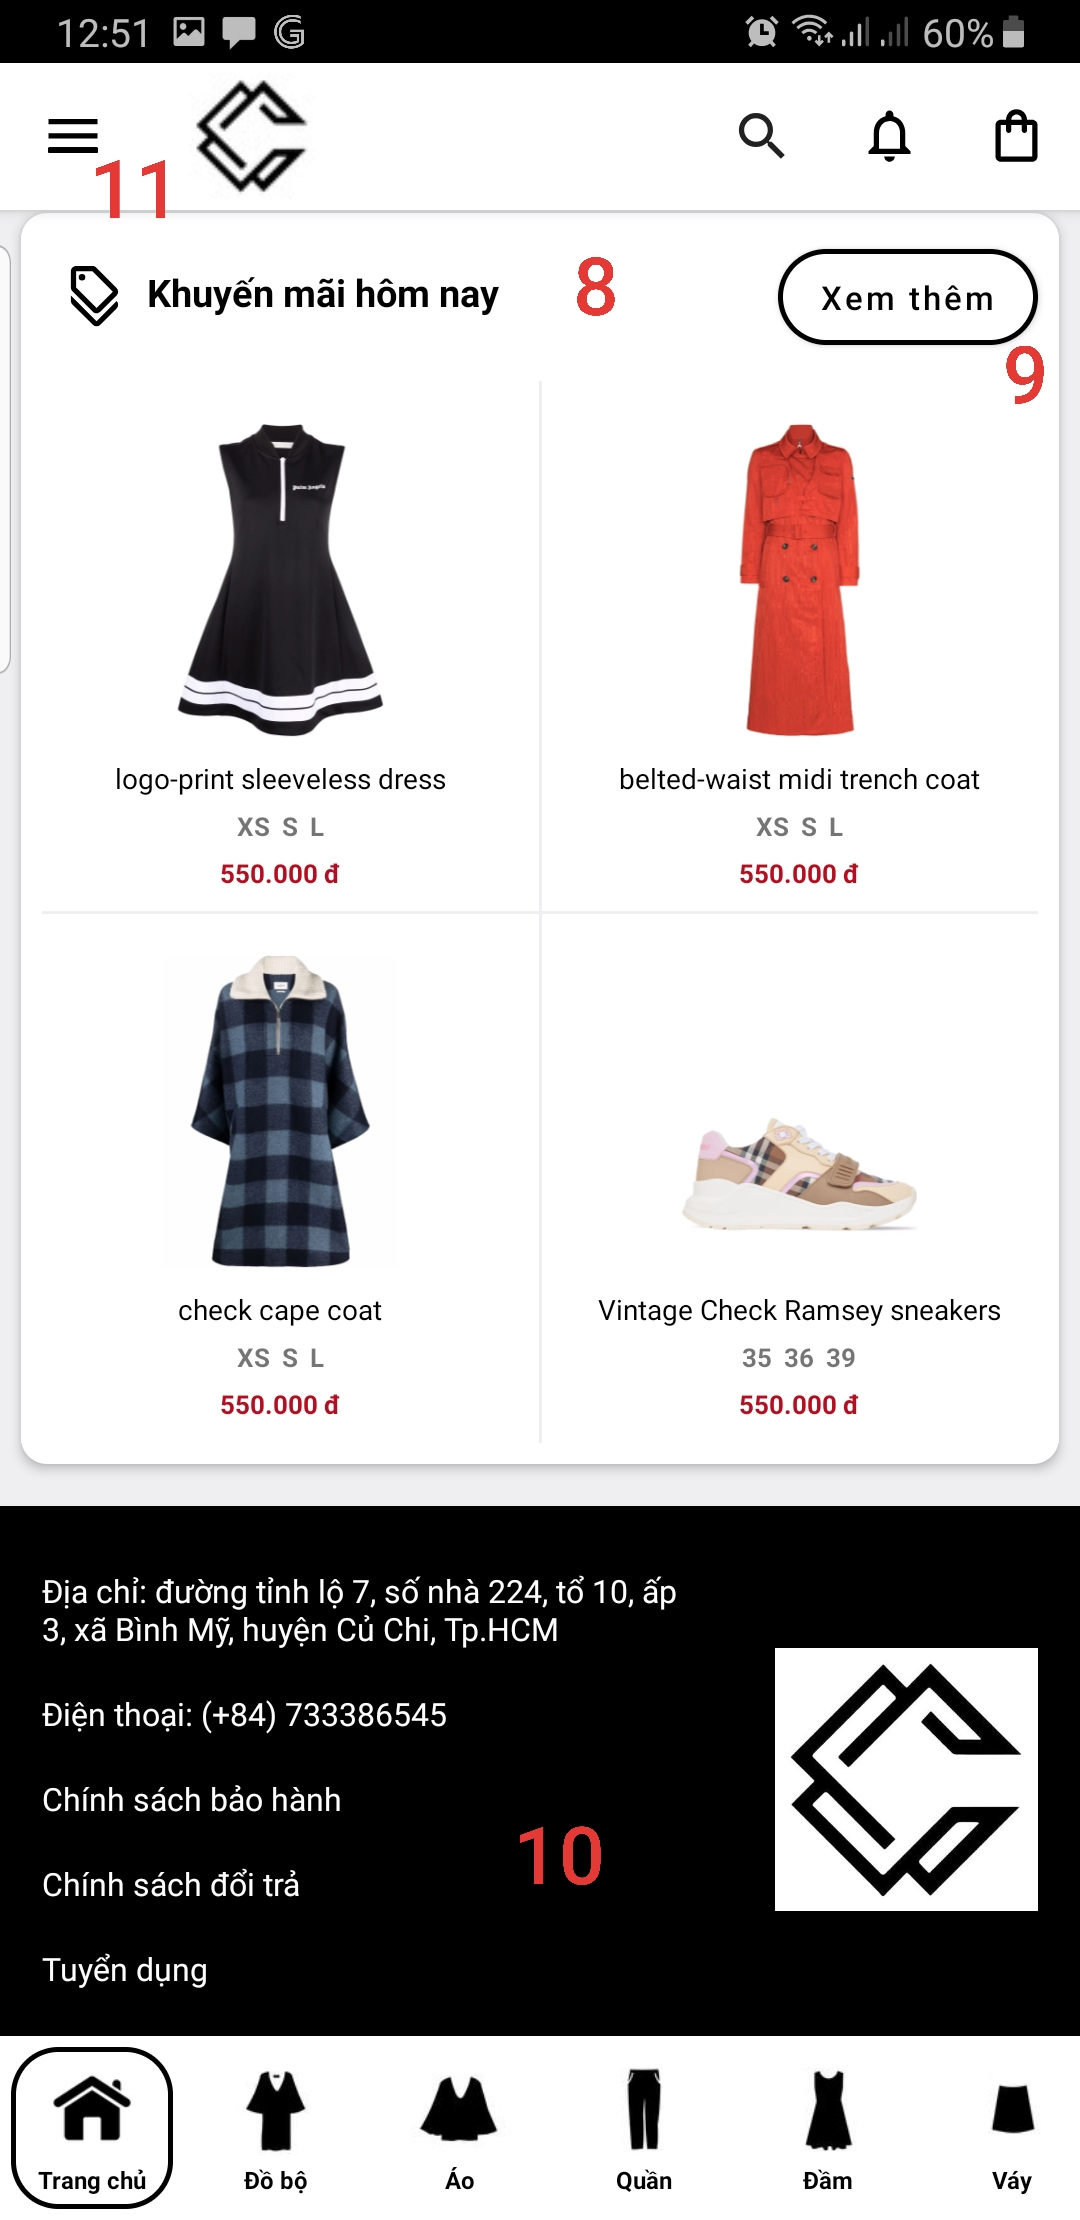
\includegraphics[height=10cm]{images/13.png}
    \caption{Màn hình trang chủ 3}
\end{figure}

\indent \textbf{Các thành phần và chức năng kèm theo trên màn hình (3)}
\begin{itemize}
    \item \textbf{8}: GridView - hiển thị bốn sản phẩm được khuyến mãi hôm nay. Nhấn vào item sẽ đứa đến trang chi tiết sản phẩm tương ứng, fragment này sẽ trình bày trong mục 2.3.4.
    \item \textbf{9}: Button - nhấn vào sẽ đưa đến một fragment khác hiển thị nhiều sản phẩm khuyến mãi hơn dưới dạng GridView, fragment này sẽ được trình bày ở mục 2.3.2.
    \item \textbf{10}: Footer - thể hiện địa chỉ, số điện thoại, các chính sách đổi trả, bảo hành của nhãn hàng.
    \item \textbf{11}: Hamburger toggle - nhấn vào để mở navigation view.
\end{itemize}

\newpage
\begin{figure}[H]
    \centering
    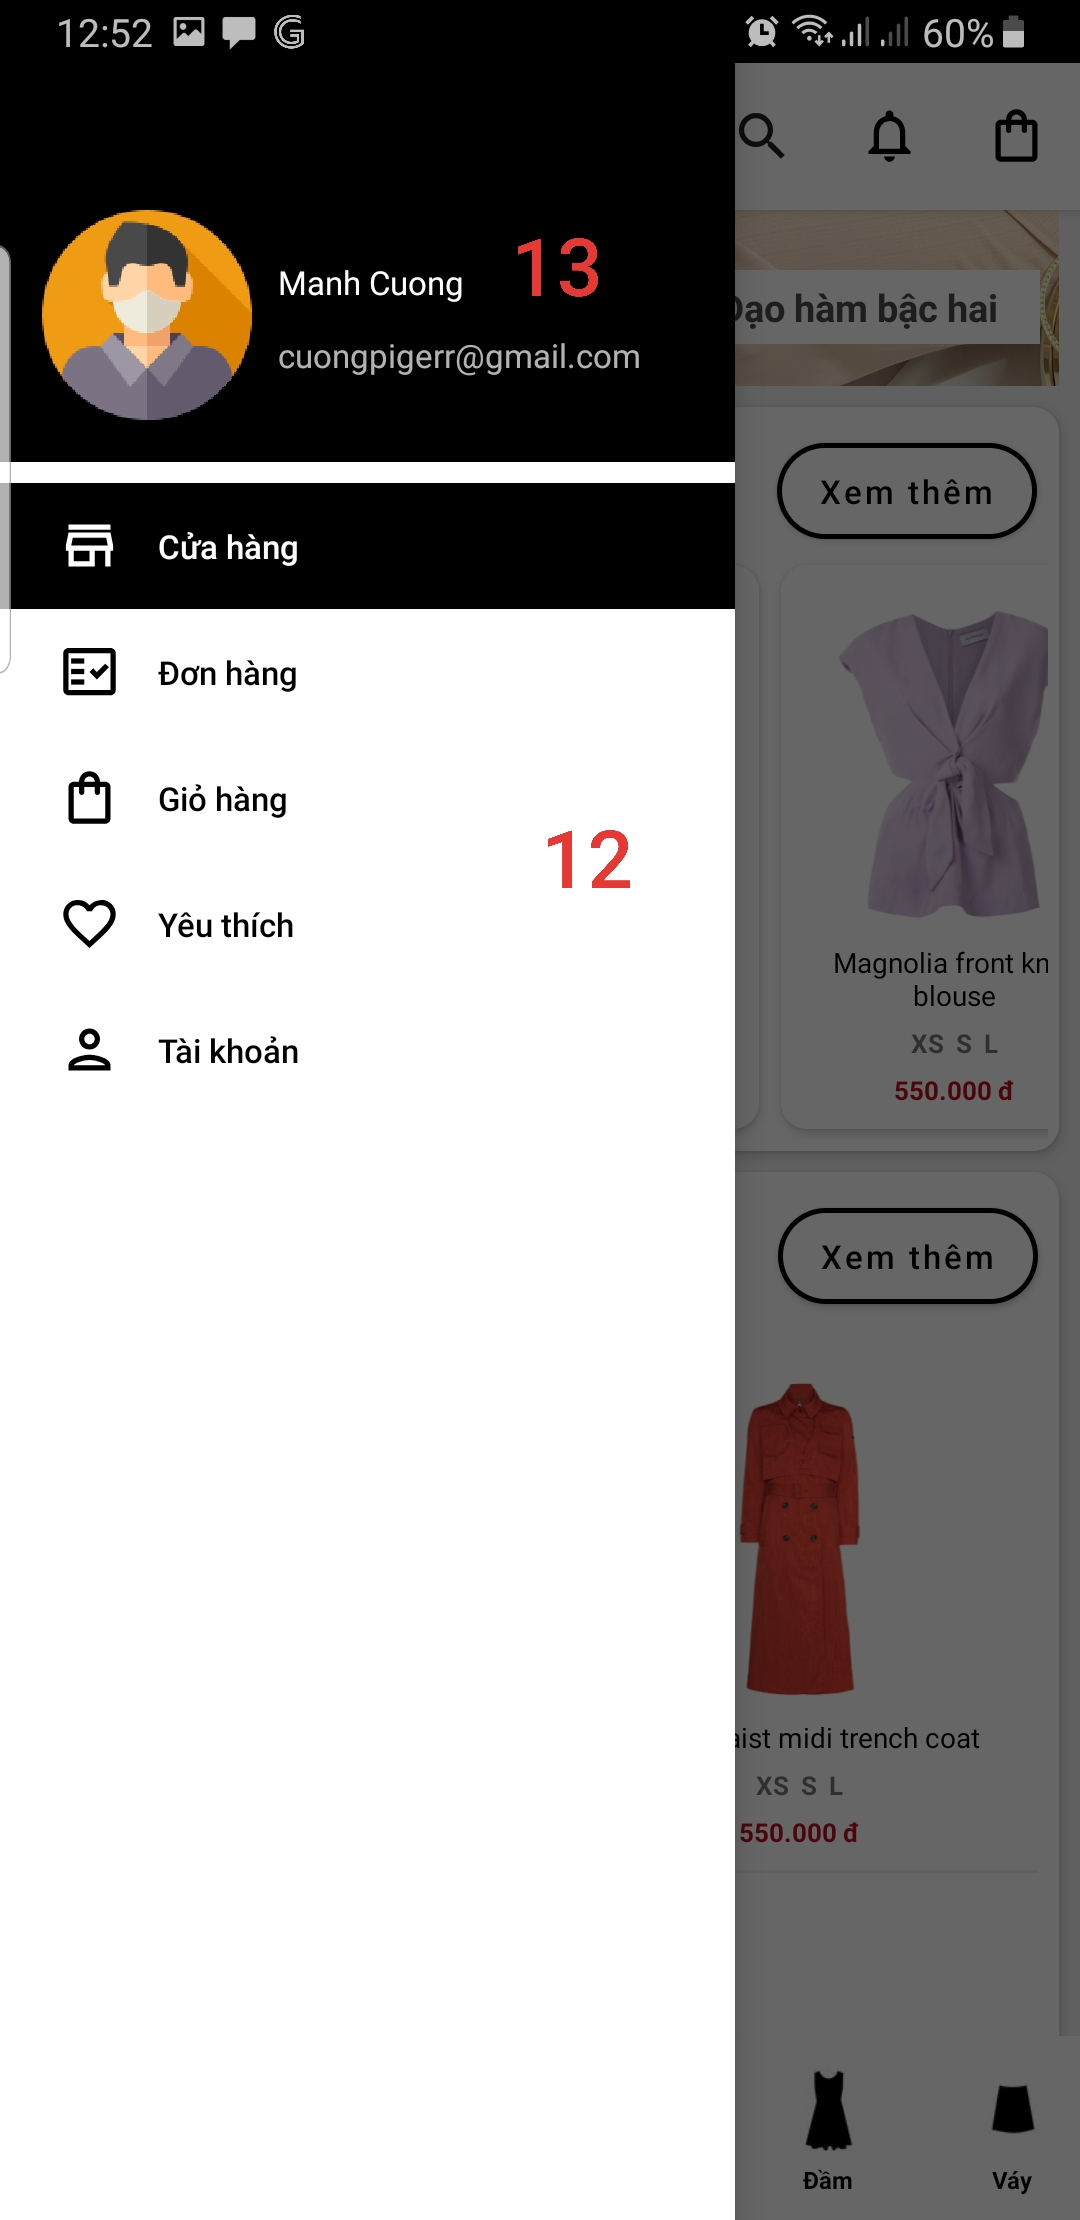
\includegraphics[height=10cm]{images/14.png}
    \caption{Màn hình trang chủ 4}
\end{figure}

\indent \textbf{Các thành phần và chức năng kèm theo trên màn hình (4)}
\begin{itemize}
    \item \textbf{12}: Navigation view - hiển thị các tab để đi đến các fragment khác của ứng dụng. Hiện tại ứng dụng đang ở fragment cửa hàng.
    \item \textbf{13}: Hai Textview - hiển thị tên người dùng và email nếu người dùng đã đăng nhập - ngược lại thì sẽ hiển thị thông báo chưa đăng nhập.
\end{itemize}

\indent \textbf{Ưu điểm}
\begin{itemize}
    \item Vì được thiết kế dưới dạng một Vertical Recycler View mà mỗi item là một container chứa tập các widget khác nhau, nên về sau ta dễ thêm bớt các container cho màn hình trang chủ.
\end{itemize}

\newpage
\subsubsection{Màn hình xem thêm sản phẩm}
Được thực hiện bởi sinh viên 20424008.\\

\indent Người dùng sẽ được đưa đến màn hình này khi nhấn vào thành phần \textbf{7} và \textbf{9} ở mục 2.3.1. Dưới đây là hình chụp màn hình này.

\begin{figure}[H]
    \centering
    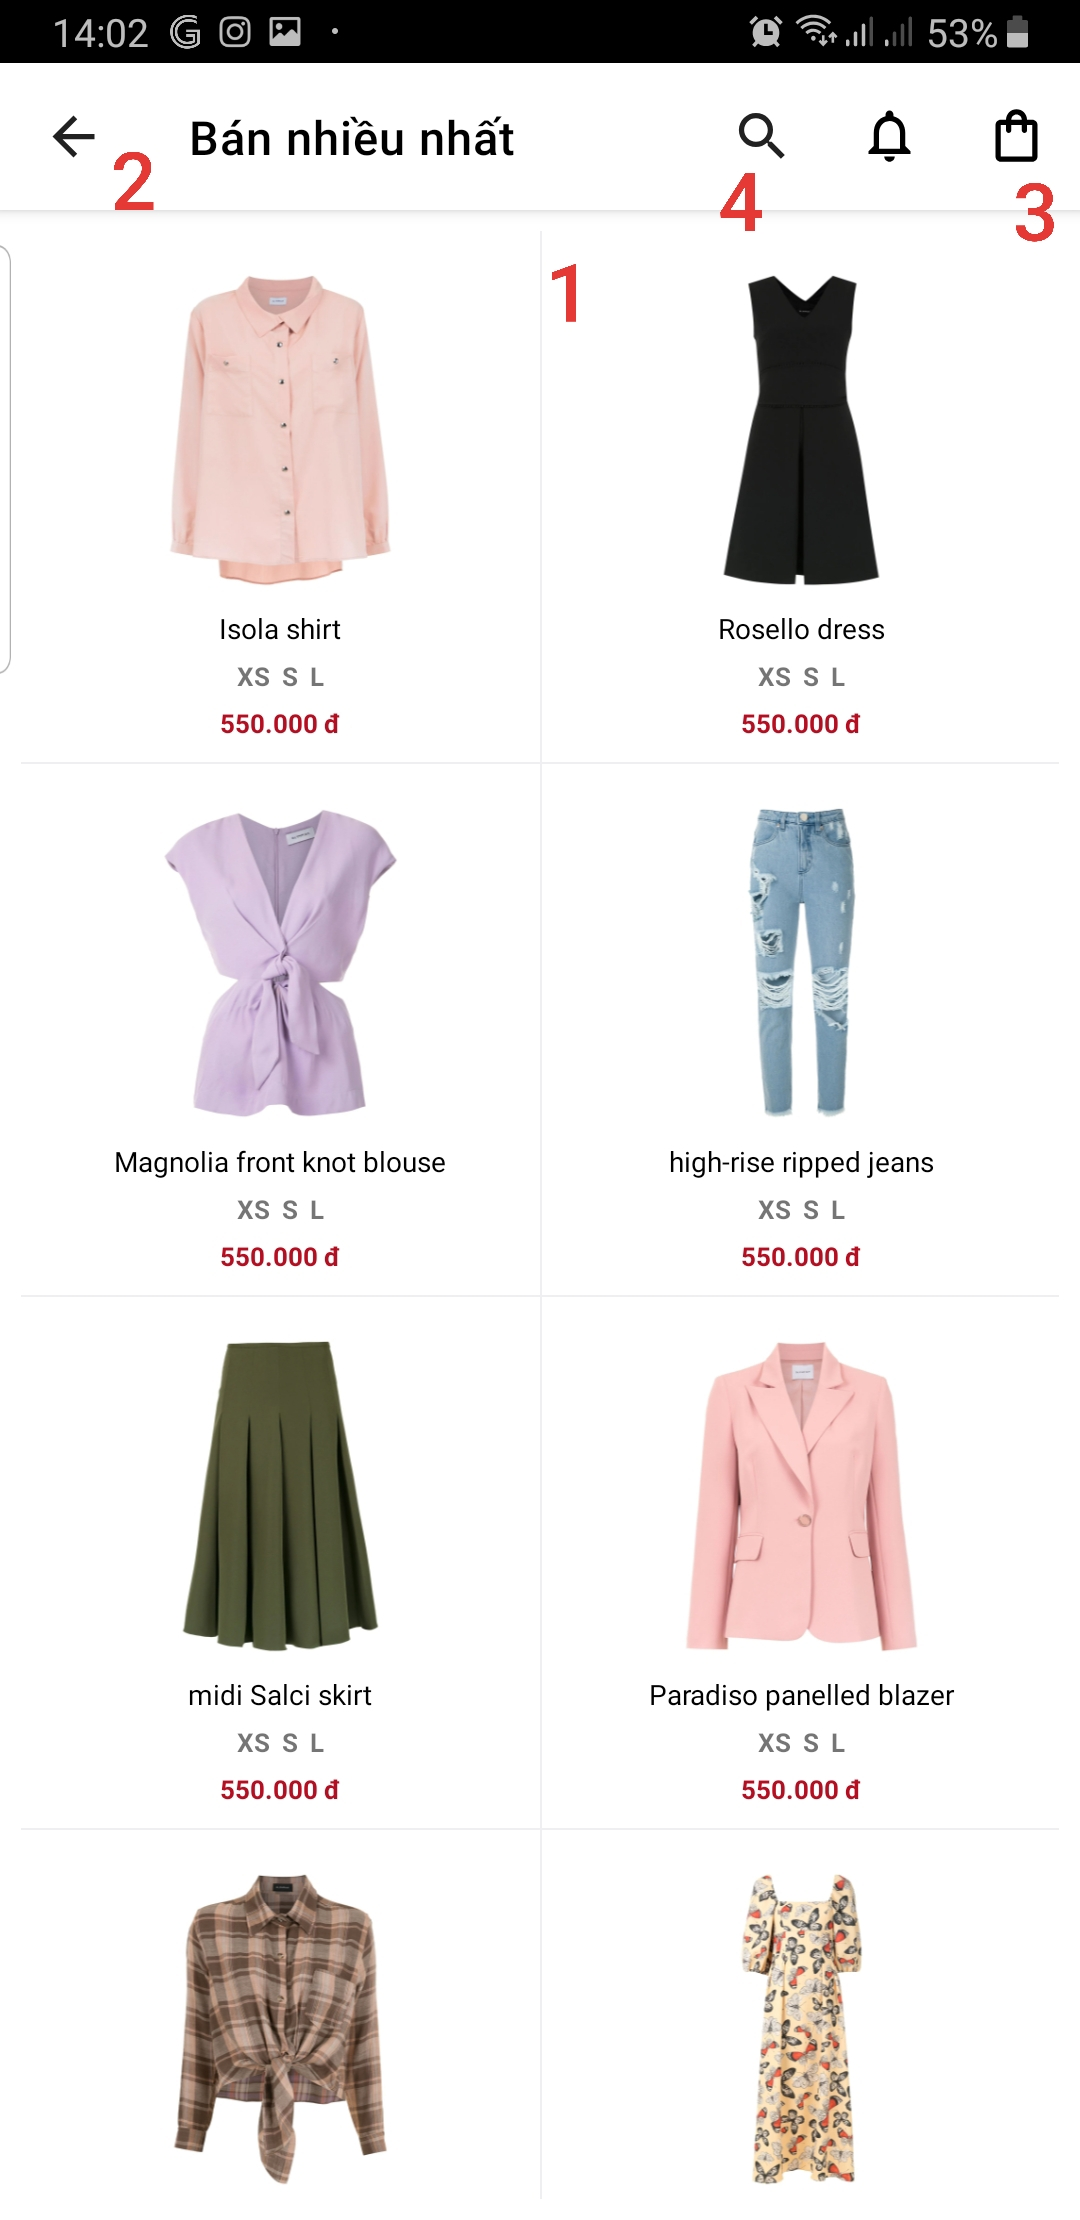
\includegraphics[height=10cm]{images/15.png}
    \caption{Màn hình xem thêm của các sản phẩm bán nhiều nhất (khi nhấn thành phần \textbf{7} ở mục 2.3.1)}
\end{figure}

\indent \textbf{Các thành phần và chức năng kèm theo trên màn hình (3)}
\begin{itemize}
    \item \textbf{1}: GridView - hiển thị nhiều hơn các sản phẩm khi người dùng nhấn vào thành phần \textbf{7} hoặc \textbf{9} ở mục 2.3.1. Có thể scroll, nhấn vào item để đi đến trang chi tiết sản phẩm tương ứng, fragment này sẽ trình bày trong mục 2.3.4.
    \item \textbf{2}: As home indicator - nhấn vào để quay về màn hình chính ở mục 2.3.1.
    \item \textbf{3}: Menu item Cart - nhấn vào để đến fragment giỏ hàng.
    \item \textbf{4}: Menu item Search - nhấn vào để thực hiện chức năng tìm kiếm.
\end{itemize}

\newpage
\indent Bên dưới là một vài hình ảnh thêm về màn hình này.

\begin{figure}[H]
    \centering
    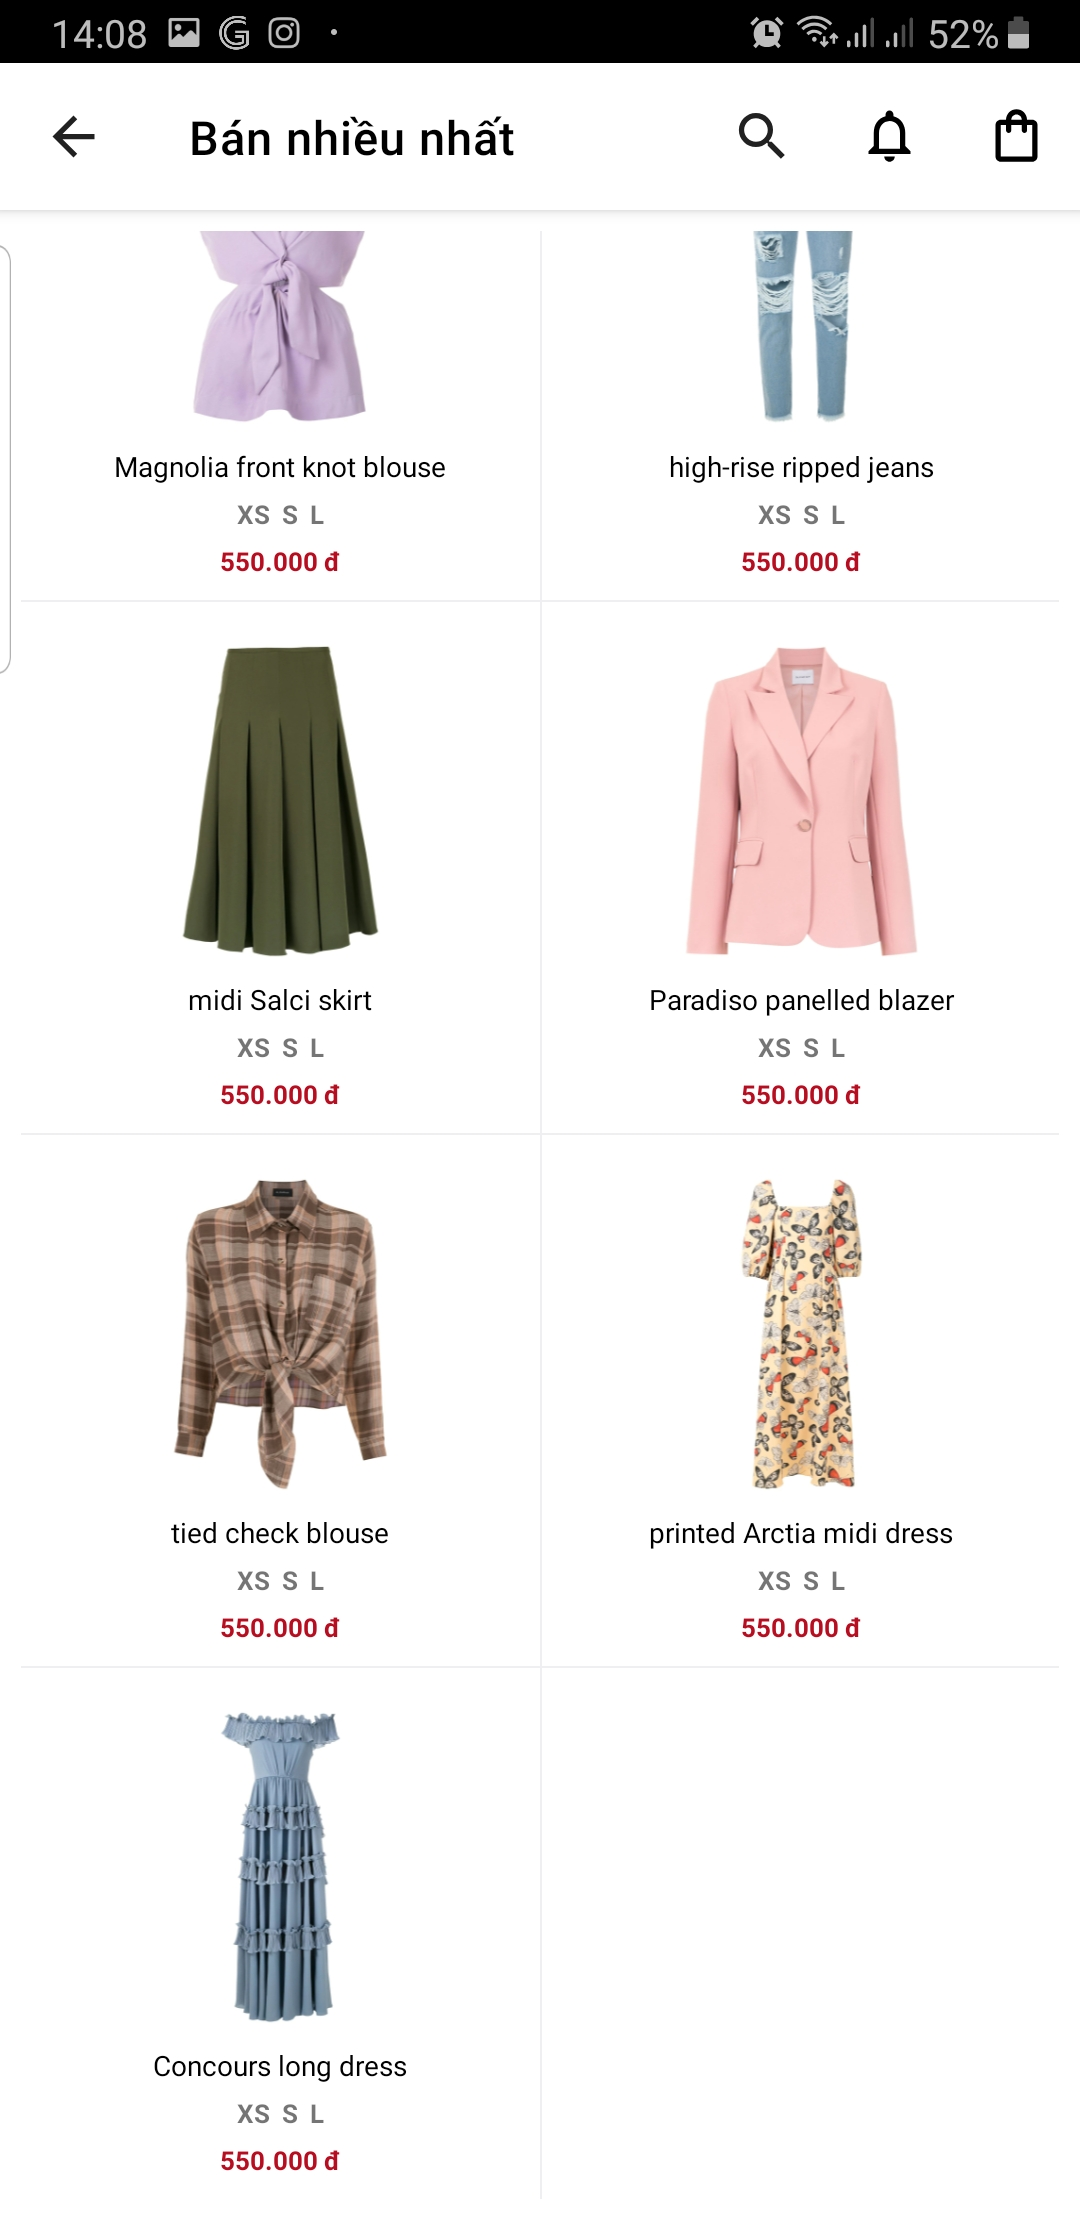
\includegraphics[height=10cm]{images/16.png}
    \caption{Màn hình xem thêm của các sản phẩm bán nhiều nhất - cuối trang (khi nhấn thành phần \textbf{7} ở mục 2.3.1)}
\end{figure}

\begin{figure}[H]
    \centering
    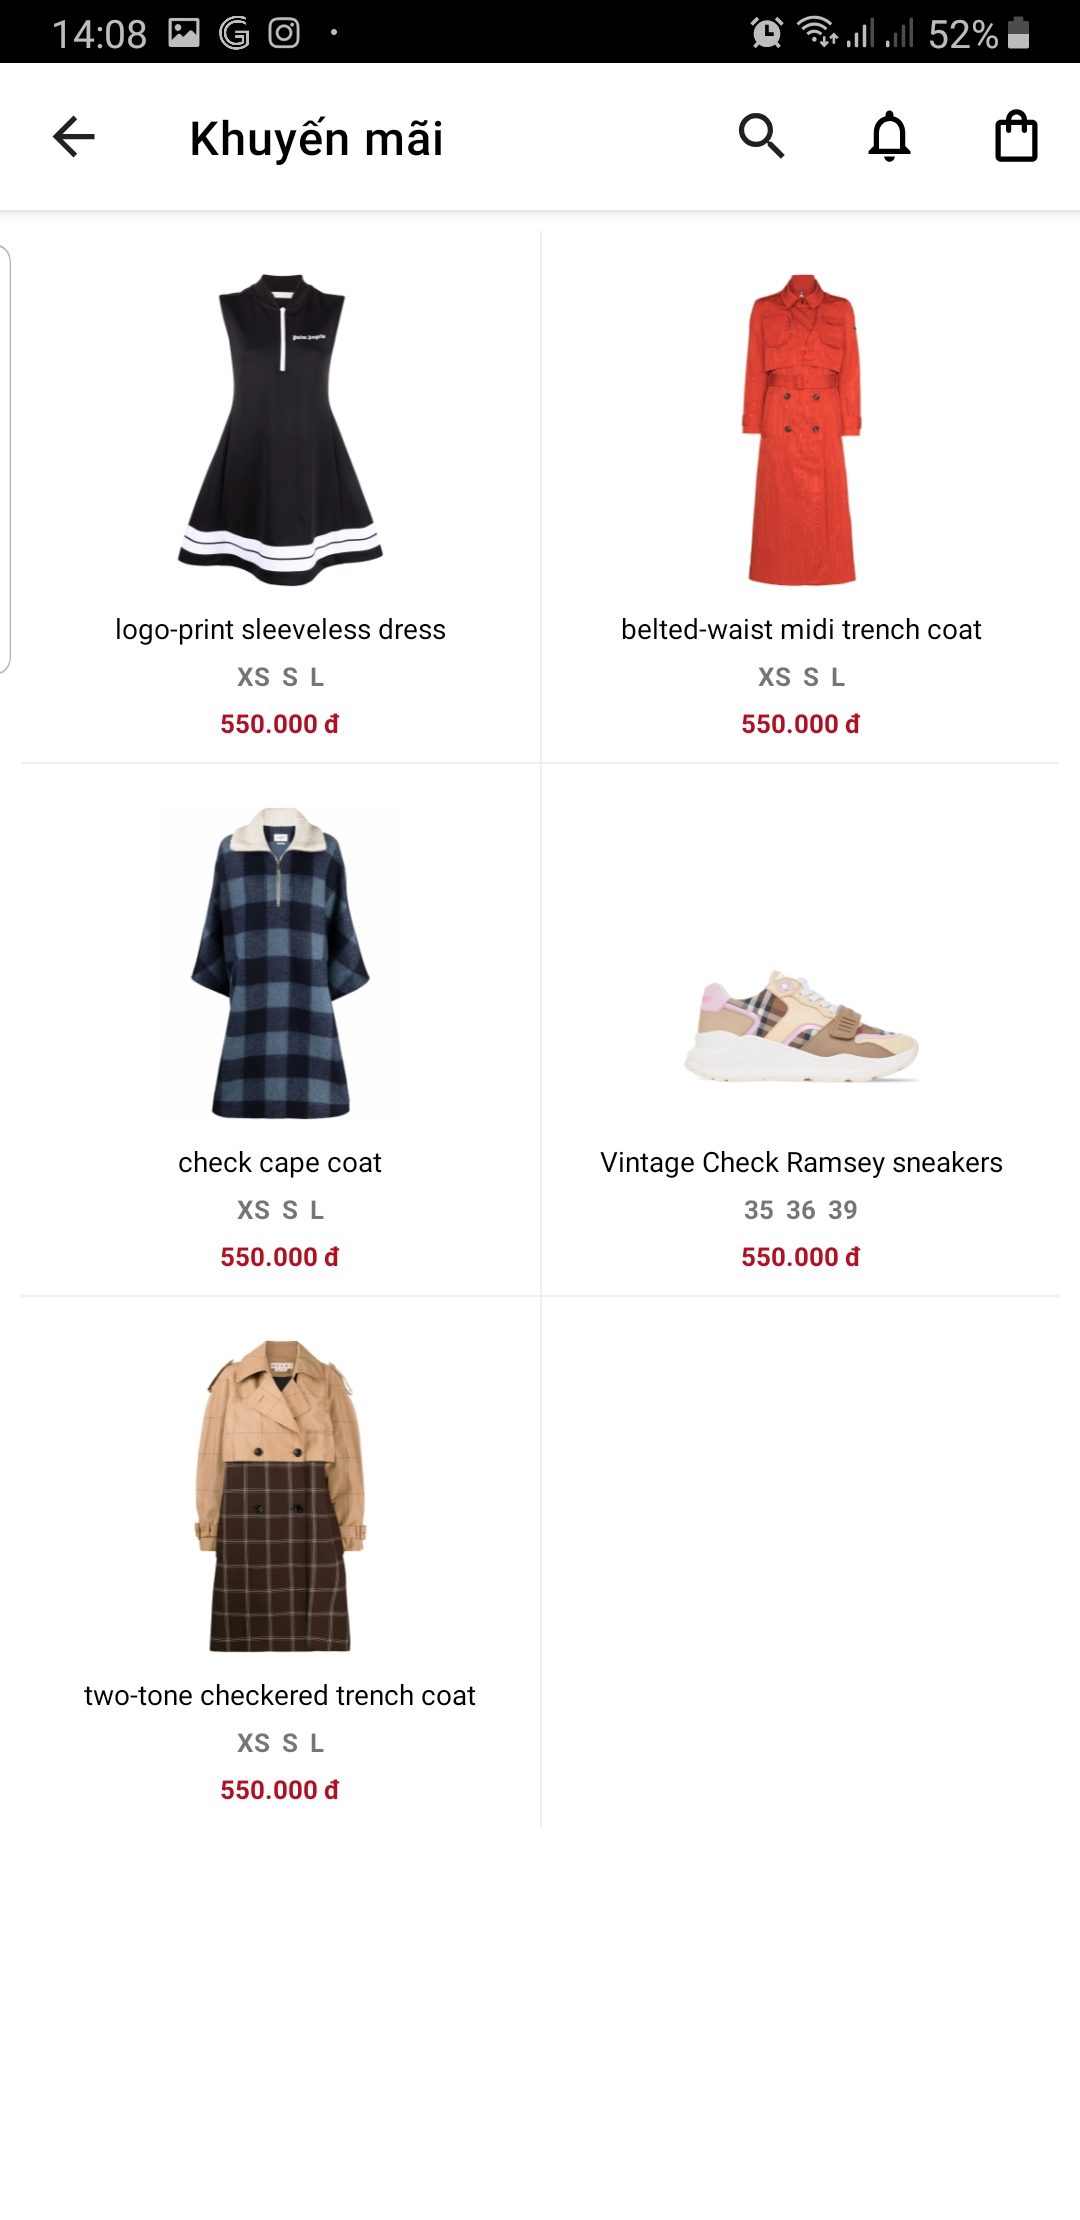
\includegraphics[height=10cm]{images/17.png}
    \caption{Màn hình xem thêm của các sản phẩm khuyến mãi (khi nhấn thành phần \textbf{9} ở mục 2.3.1)}
\end{figure}

\newpage
\subsubsection{Màn hình sản phẩm theo danh mục}
Được thực hiện bởi sinh viên 20424008.\\

\indent Màn hình này được chuyển đến khi người dùng nhấn vào các item trên thành phần \textbf{2} ở mục 2.3.1. Dưới đây là hình chụp màn hình này.

\begin{figure}[H]
    \centering
    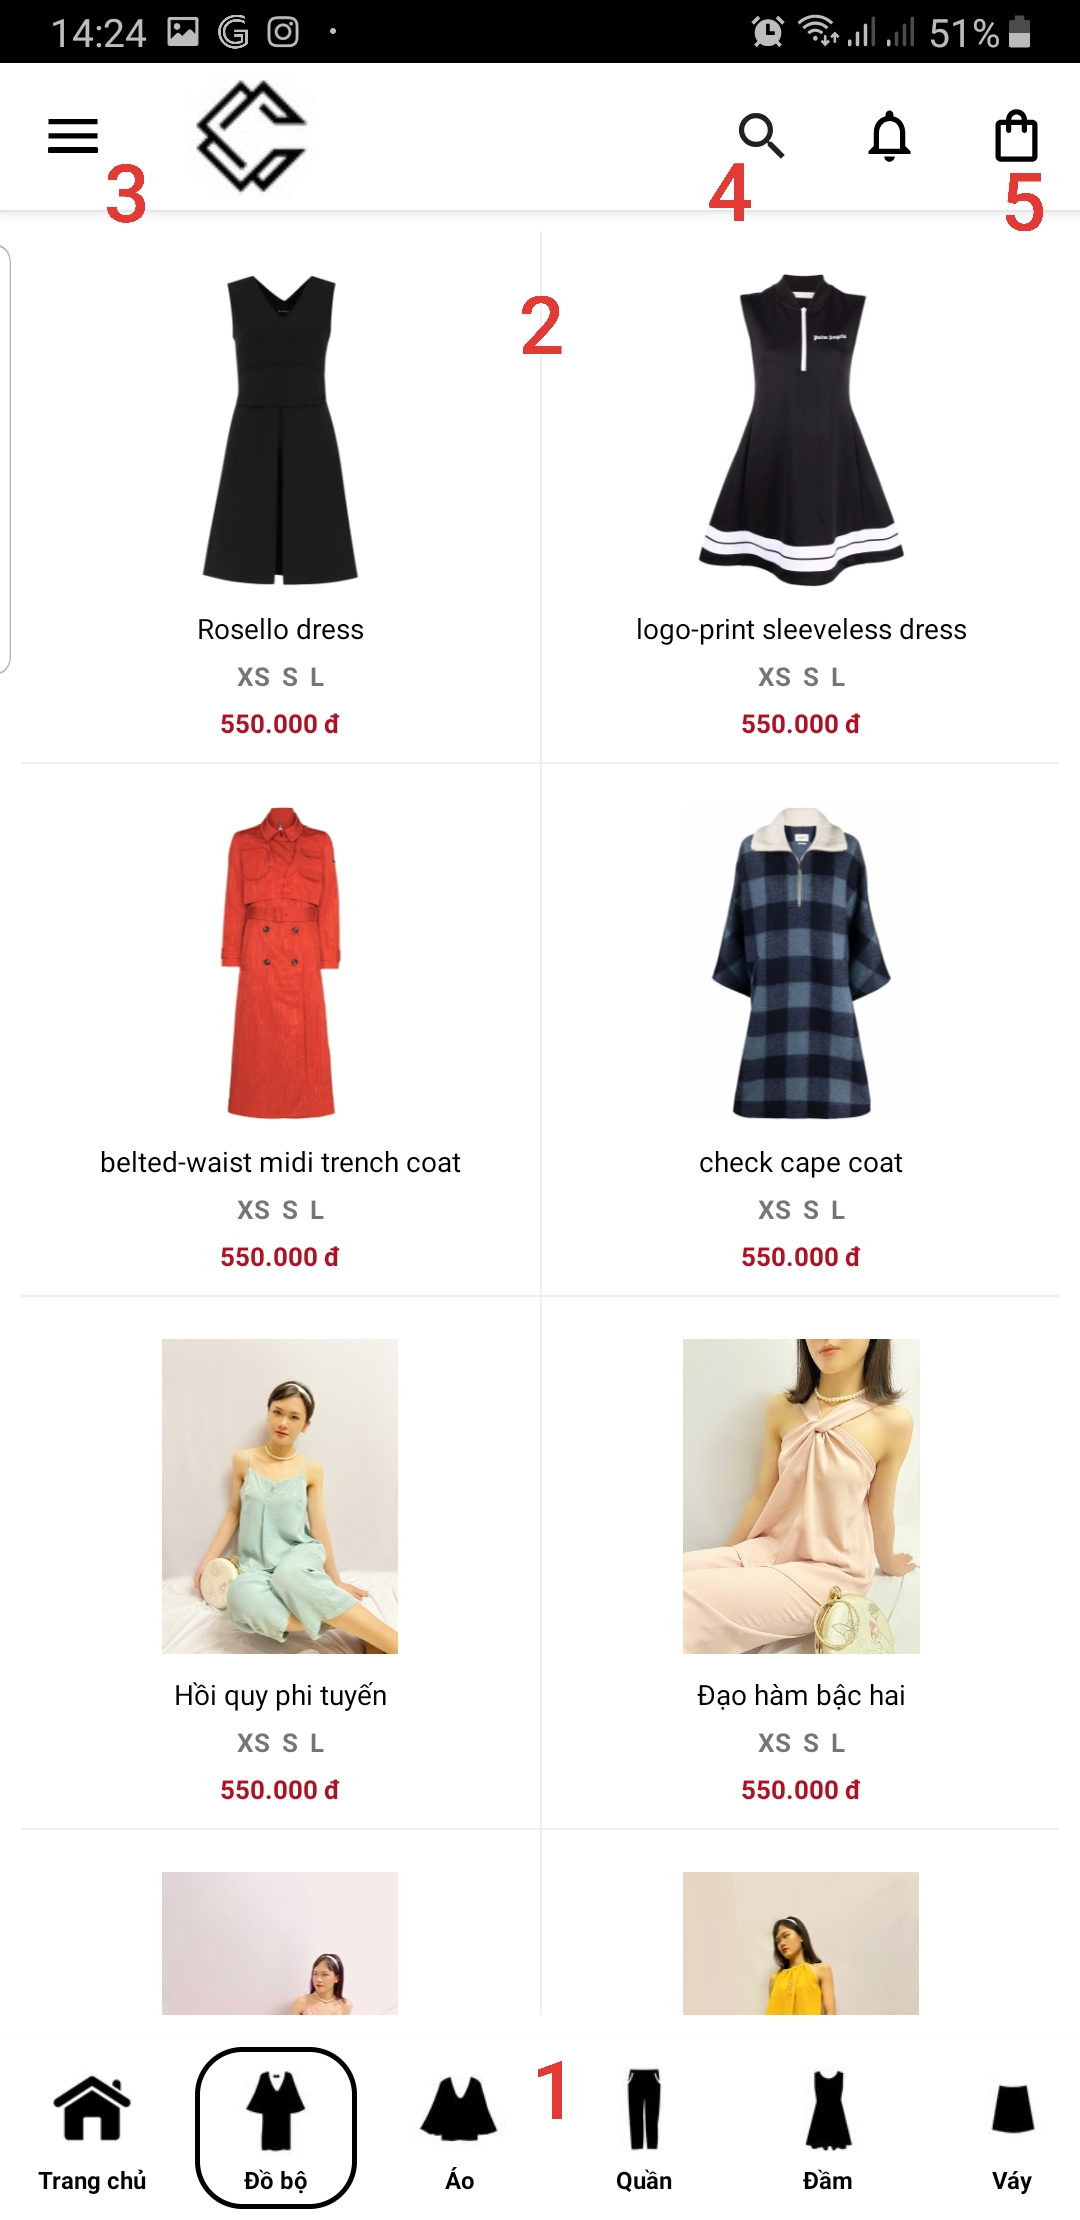
\includegraphics[height=10cm]{images/18.png}
    \caption{Màn hình xem các sản phẩm theo danh mục - danh mục "Đồ bộ"}
\end{figure}

\indent \textbf{Các thành phần và chức năng kèm theo trên màn hình}
\begin{itemize}
    \item \textbf{1}: Horizontal Recycler View - nhấn vào các item để đi đến các fragment của các danh mục sản phẩm khác
    \item \textbf{2}: GirdView - có thể scroll, nhấn vào các item để đi đến fragment chi tiết sản phẩm tương ứng, fragment này sẽ trình bày trong mục 2.3.4.
    \item \textbf{3}: Hamburger Toggle - nhấn để mở navigation view.
    \item \textbf{4}: Menu item Search - nhấn vào để thực hiện chức năng tìm kiếm.
    \item \textbf{5}: Menu item Cart - nhấn vào để đến fragment giỏ hàng.
\end{itemize}

\newpage
\indent Dưới đây là một vài hình ảnh thêm về màn hình này.
\begin{figure}[H]
    \centering
    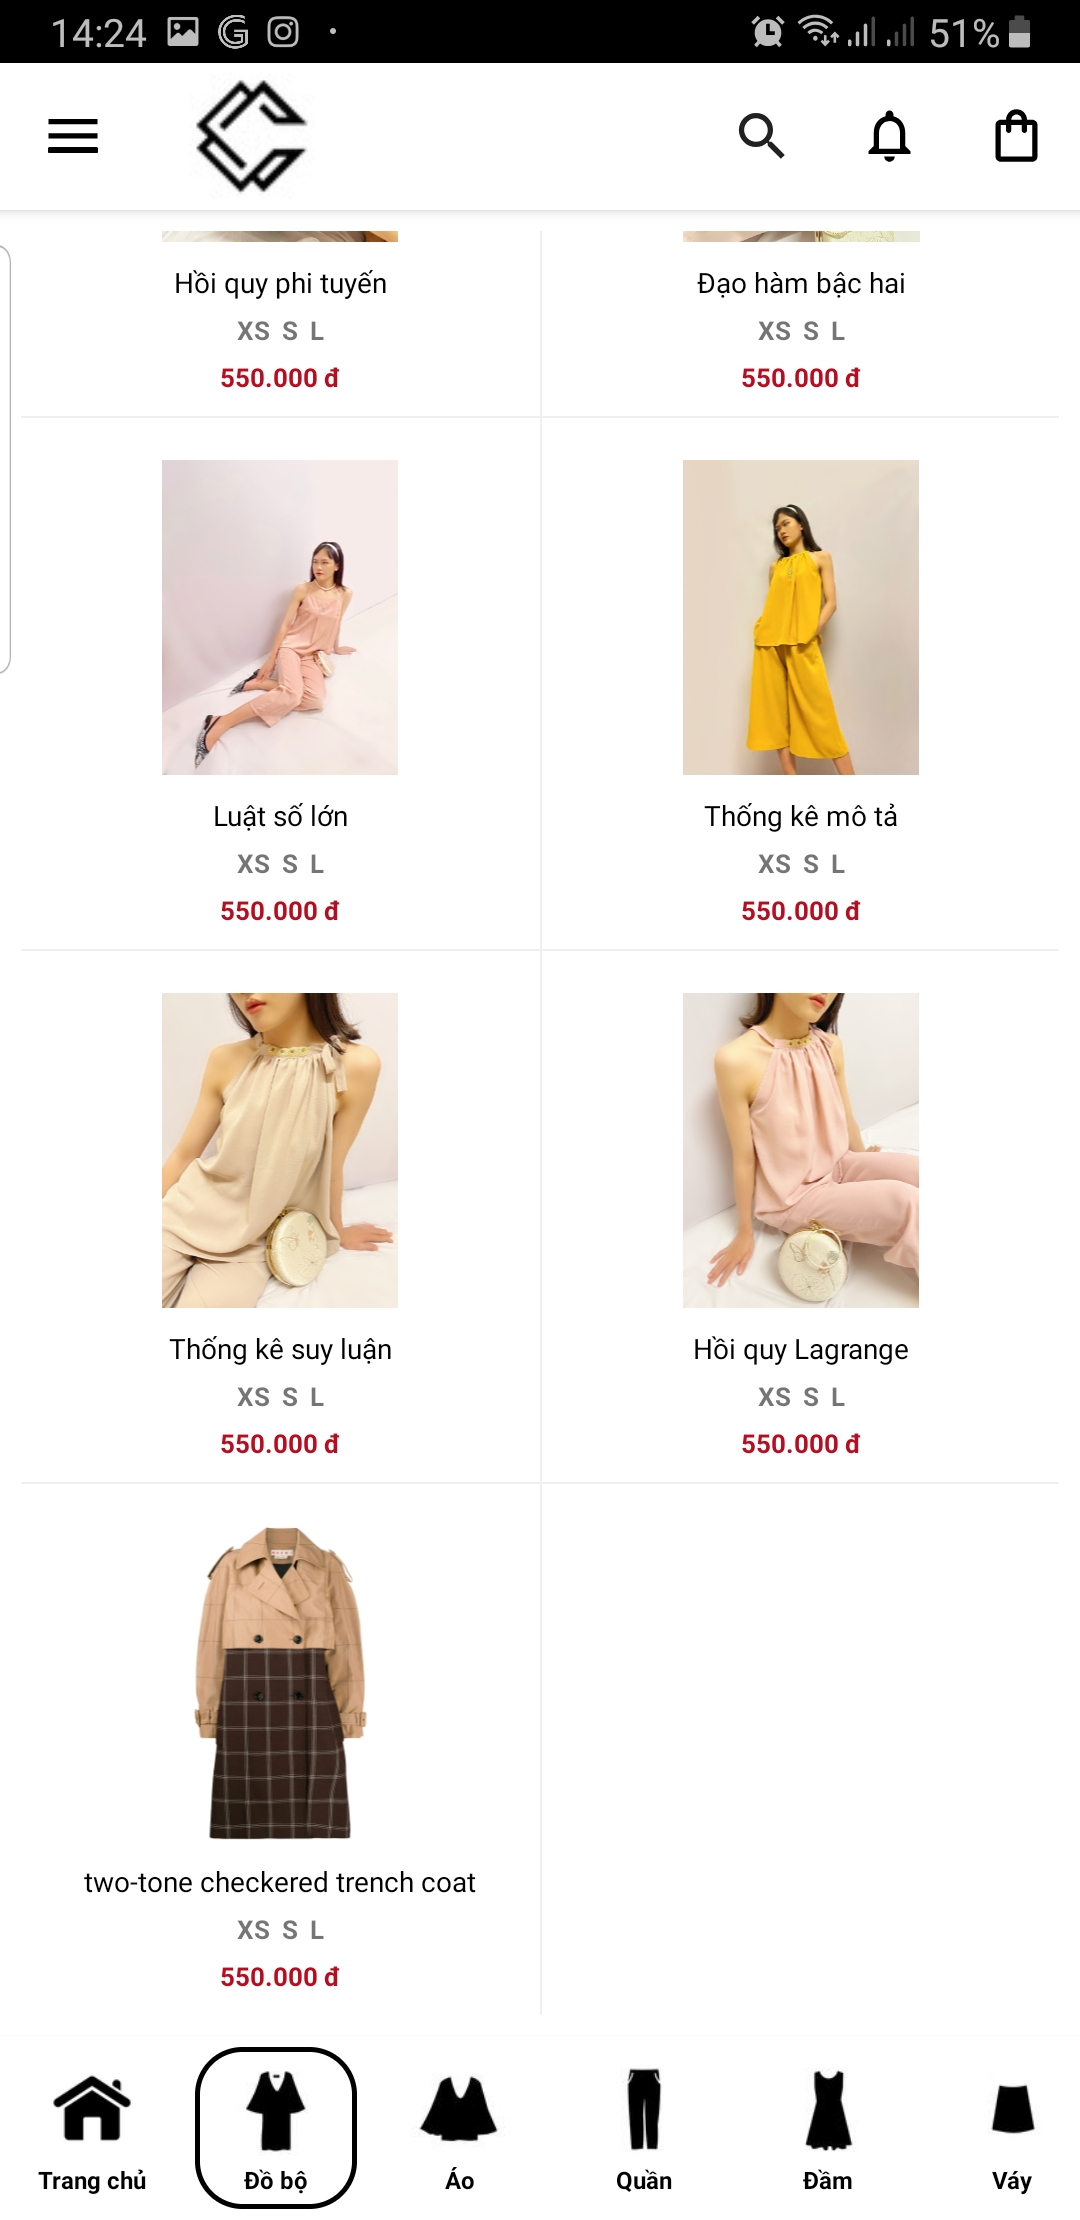
\includegraphics[height=10cm]{images/19.png}
    \caption{Màn hình xem các sản phẩm theo danh mục - cuối trang danh mục "Đồ bộ"}
\end{figure}

\begin{figure}[H]
    \centering
    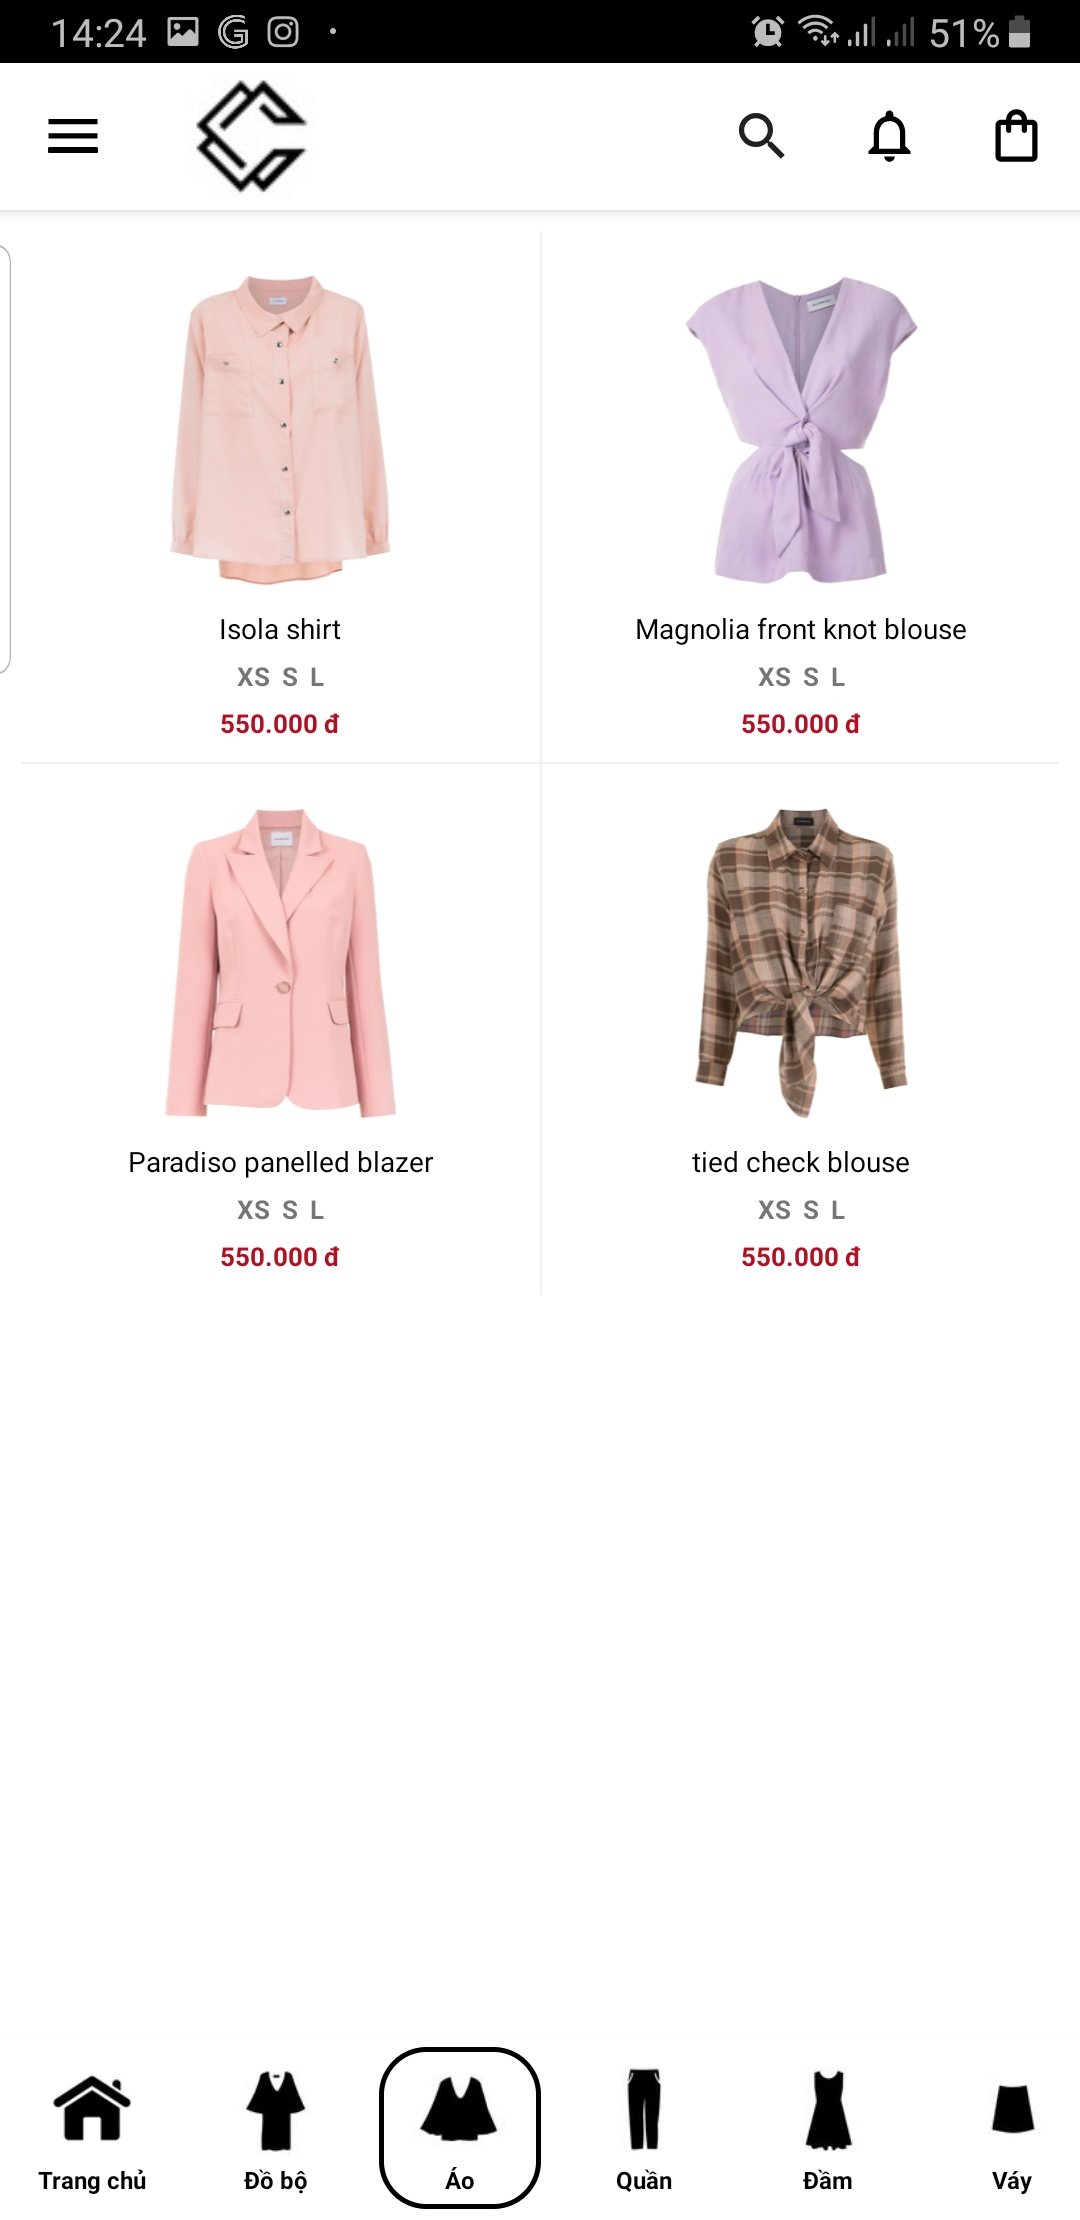
\includegraphics[height=10cm]{images/20.png}
    \caption{Màn hình xem các sản phẩm theo danh mục - danh mục "Áo"}
\end{figure}

\indent \textbf{Hạn chế}
\begin{itemize}
    \item Chưa có tính năng sắp xếp theo tiếu chí người dùng.
    \item Chưa có tính năng \textbf{Pull to load more} khi danh mục sản phẩm có nhiều sản phẩm, mặc định ứng dụng sẽ load toàn bộ sản phẩm tương ứng cho danh mục mà người dùng chọn.
\end{itemize}

\subsubsection{Màn hình chi tiết sản phẩm}
Được thực hiện bởi sinh viên 20424013.\\

\indent Màn hình này được chuyển đến khi người dùng nhấn vào các item của các thành phần \textbf{5, 6, 8} trong mục 2.3.1, thành phần \textbf{1} trong mục 2.3.2, thành phần \textbf{2} trong mục 2.3.3. Dưới đây là hình chụp màn hình này.

\begin{figure}[H]
    \centering
    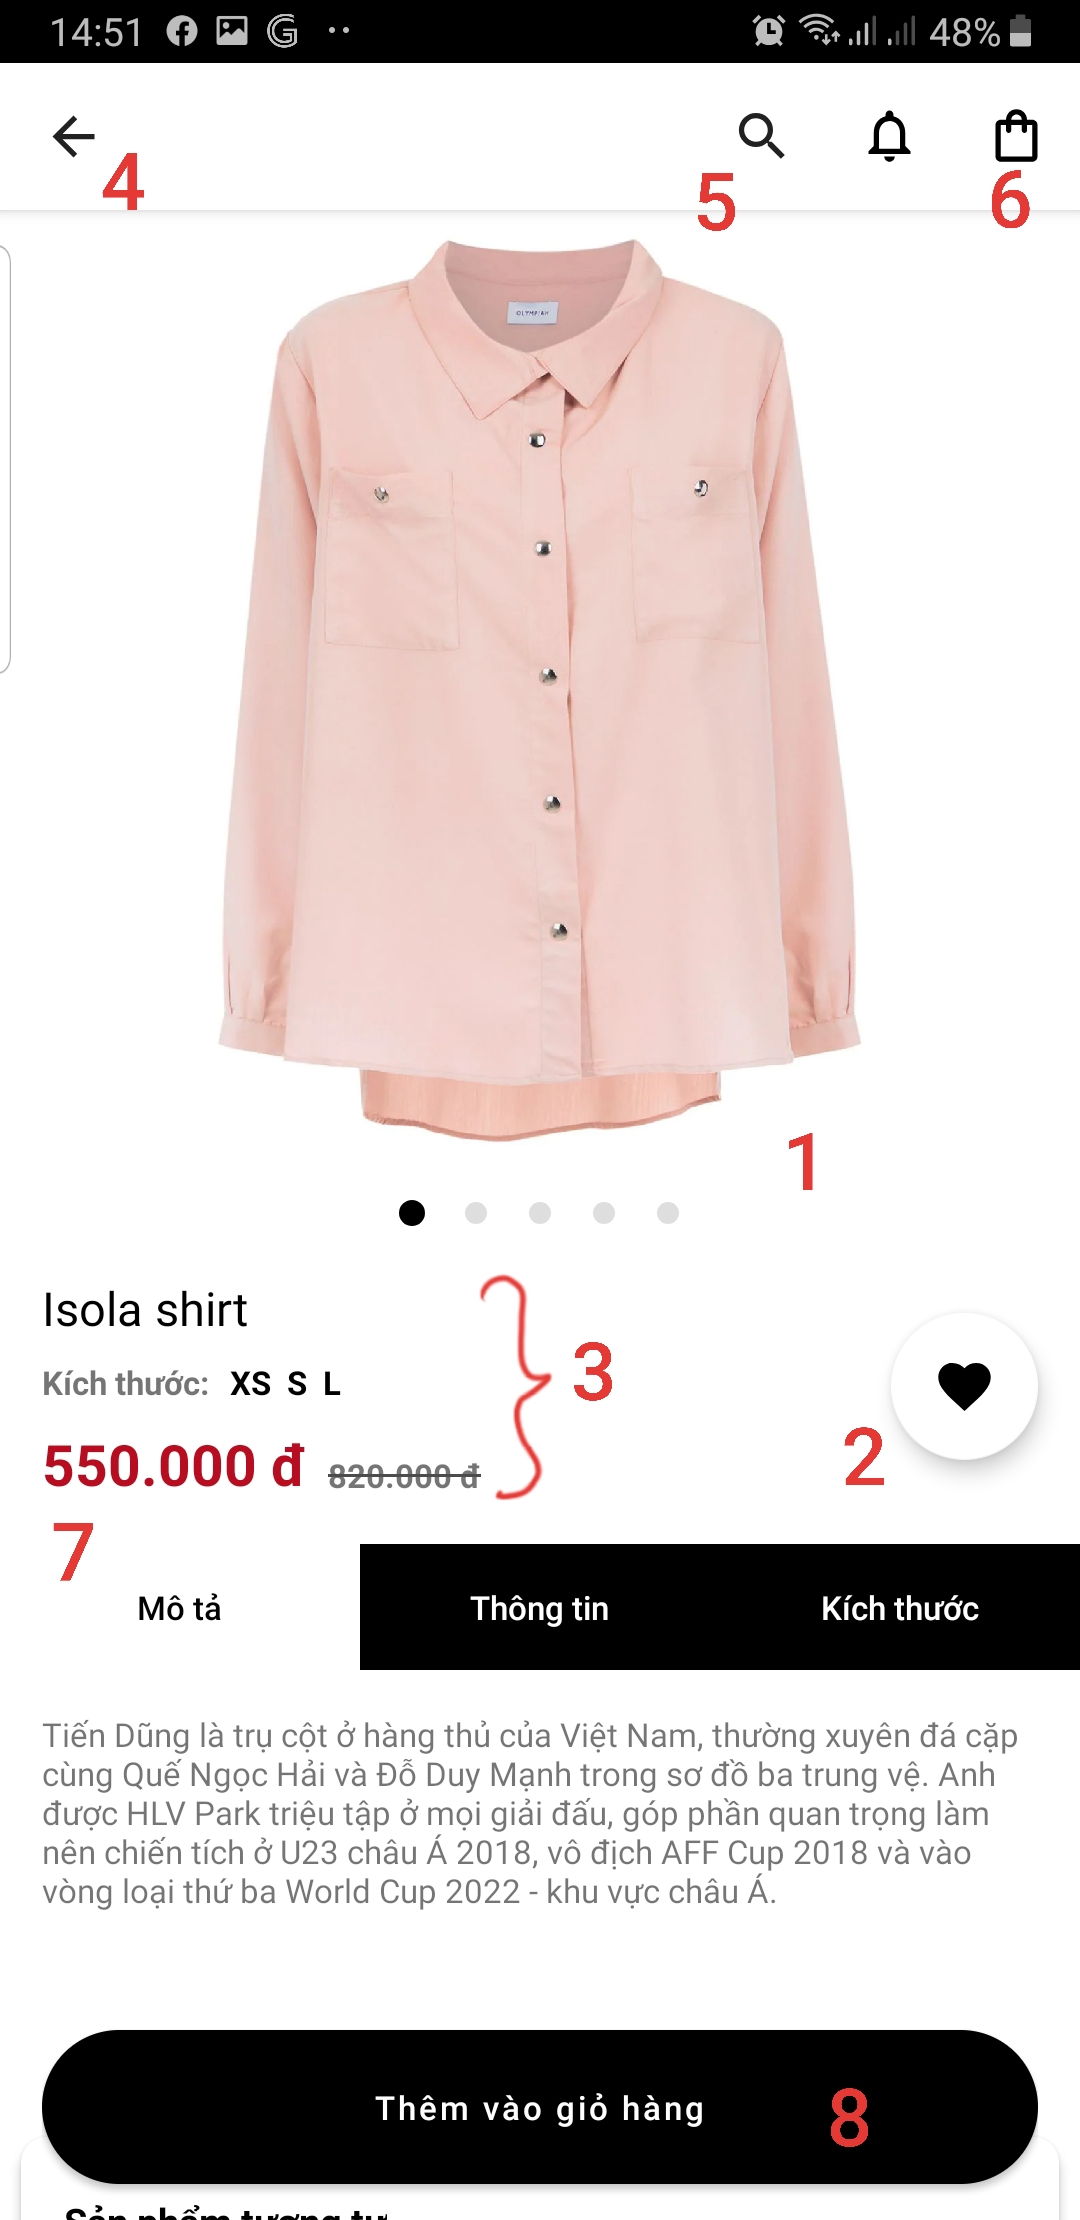
\includegraphics[height=10cm]{images/21.png}
    \caption{Màn hình chi tiết sản phẩm 1}
\end{figure}

\begin{figure}[H]
    \centering
    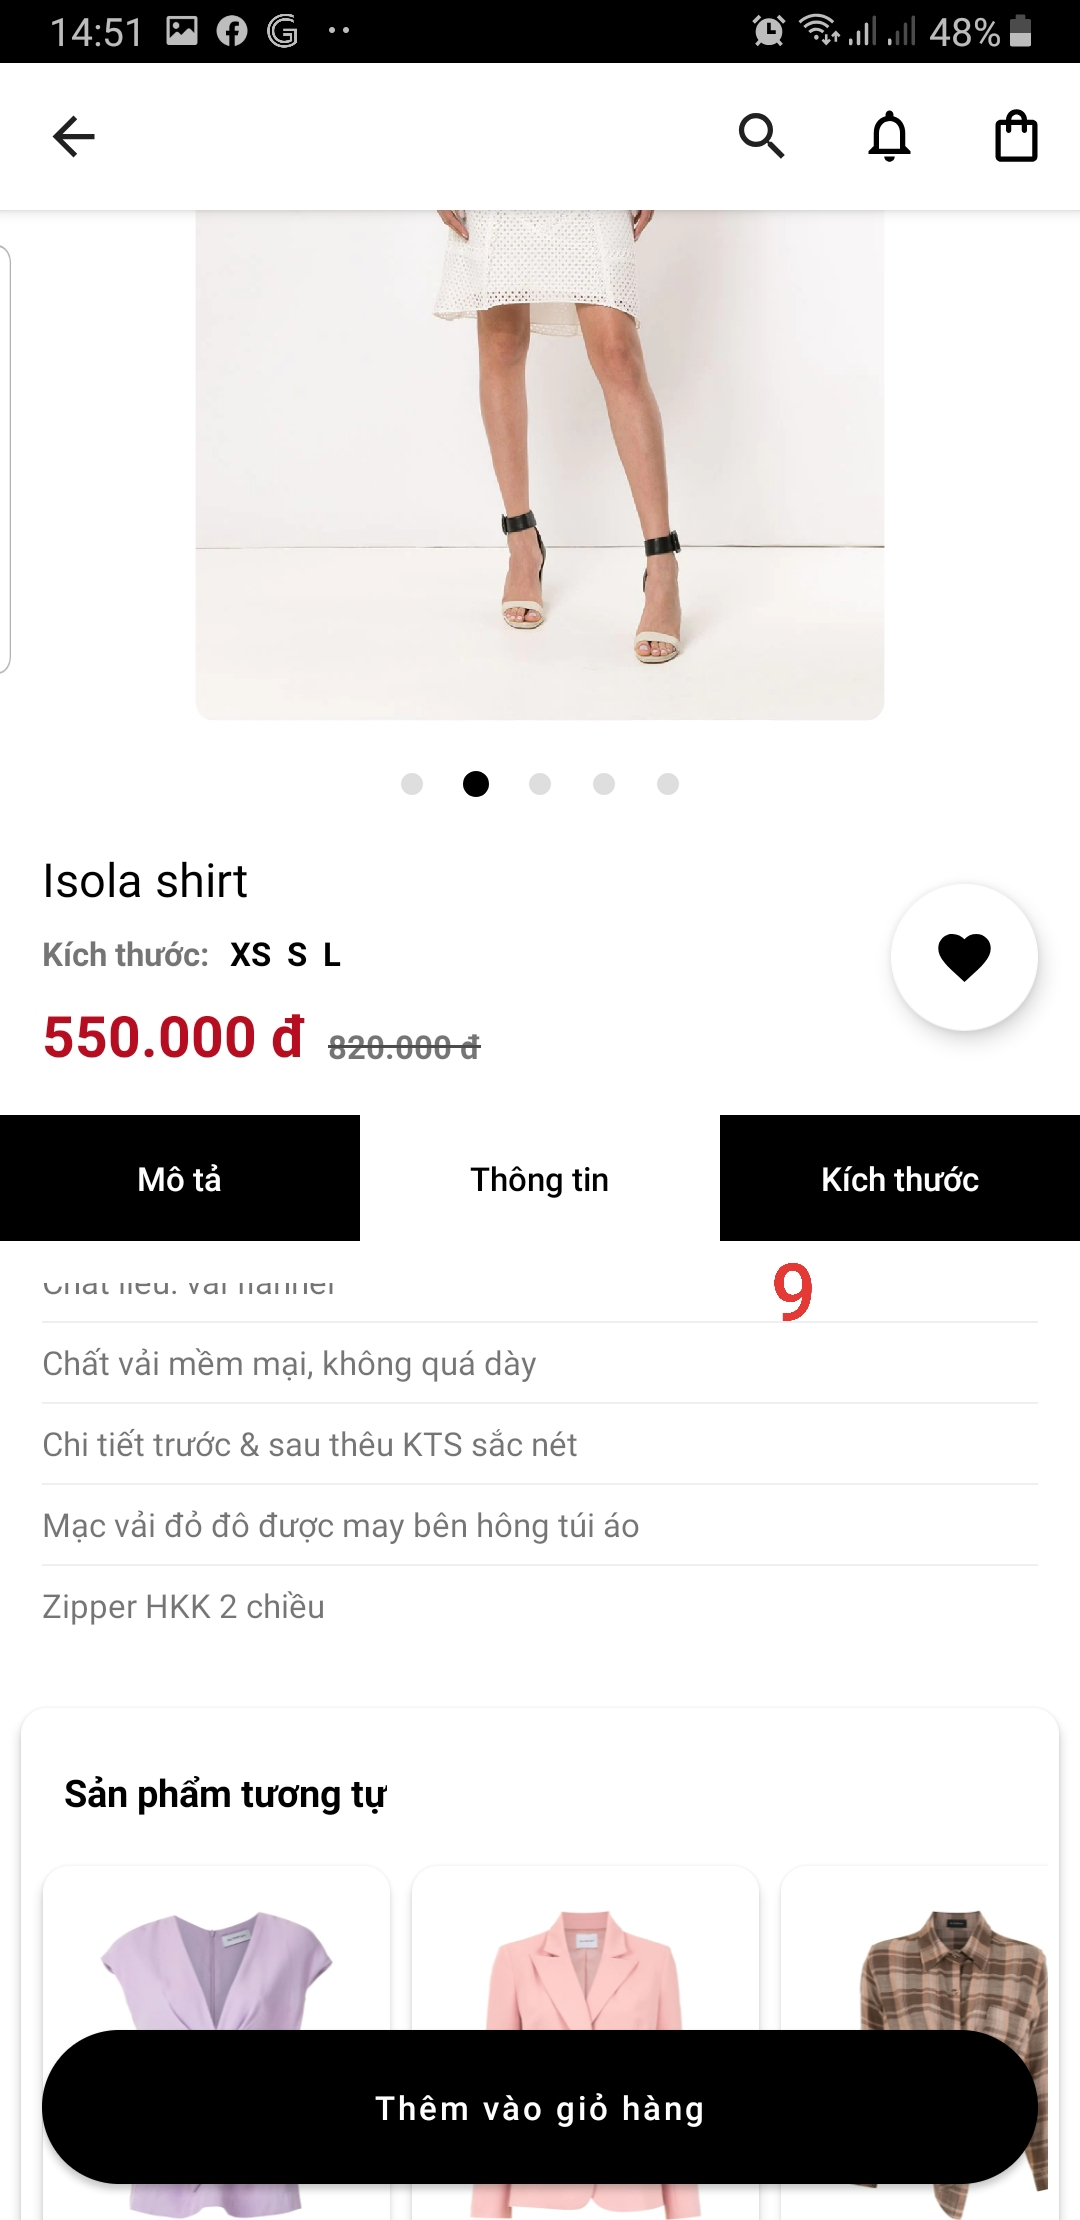
\includegraphics[height=10cm]{images/22.png}
    \caption{Màn hình chi tiết sản phẩm 2}
\end{figure}

\begin{figure}[H]
    \centering
    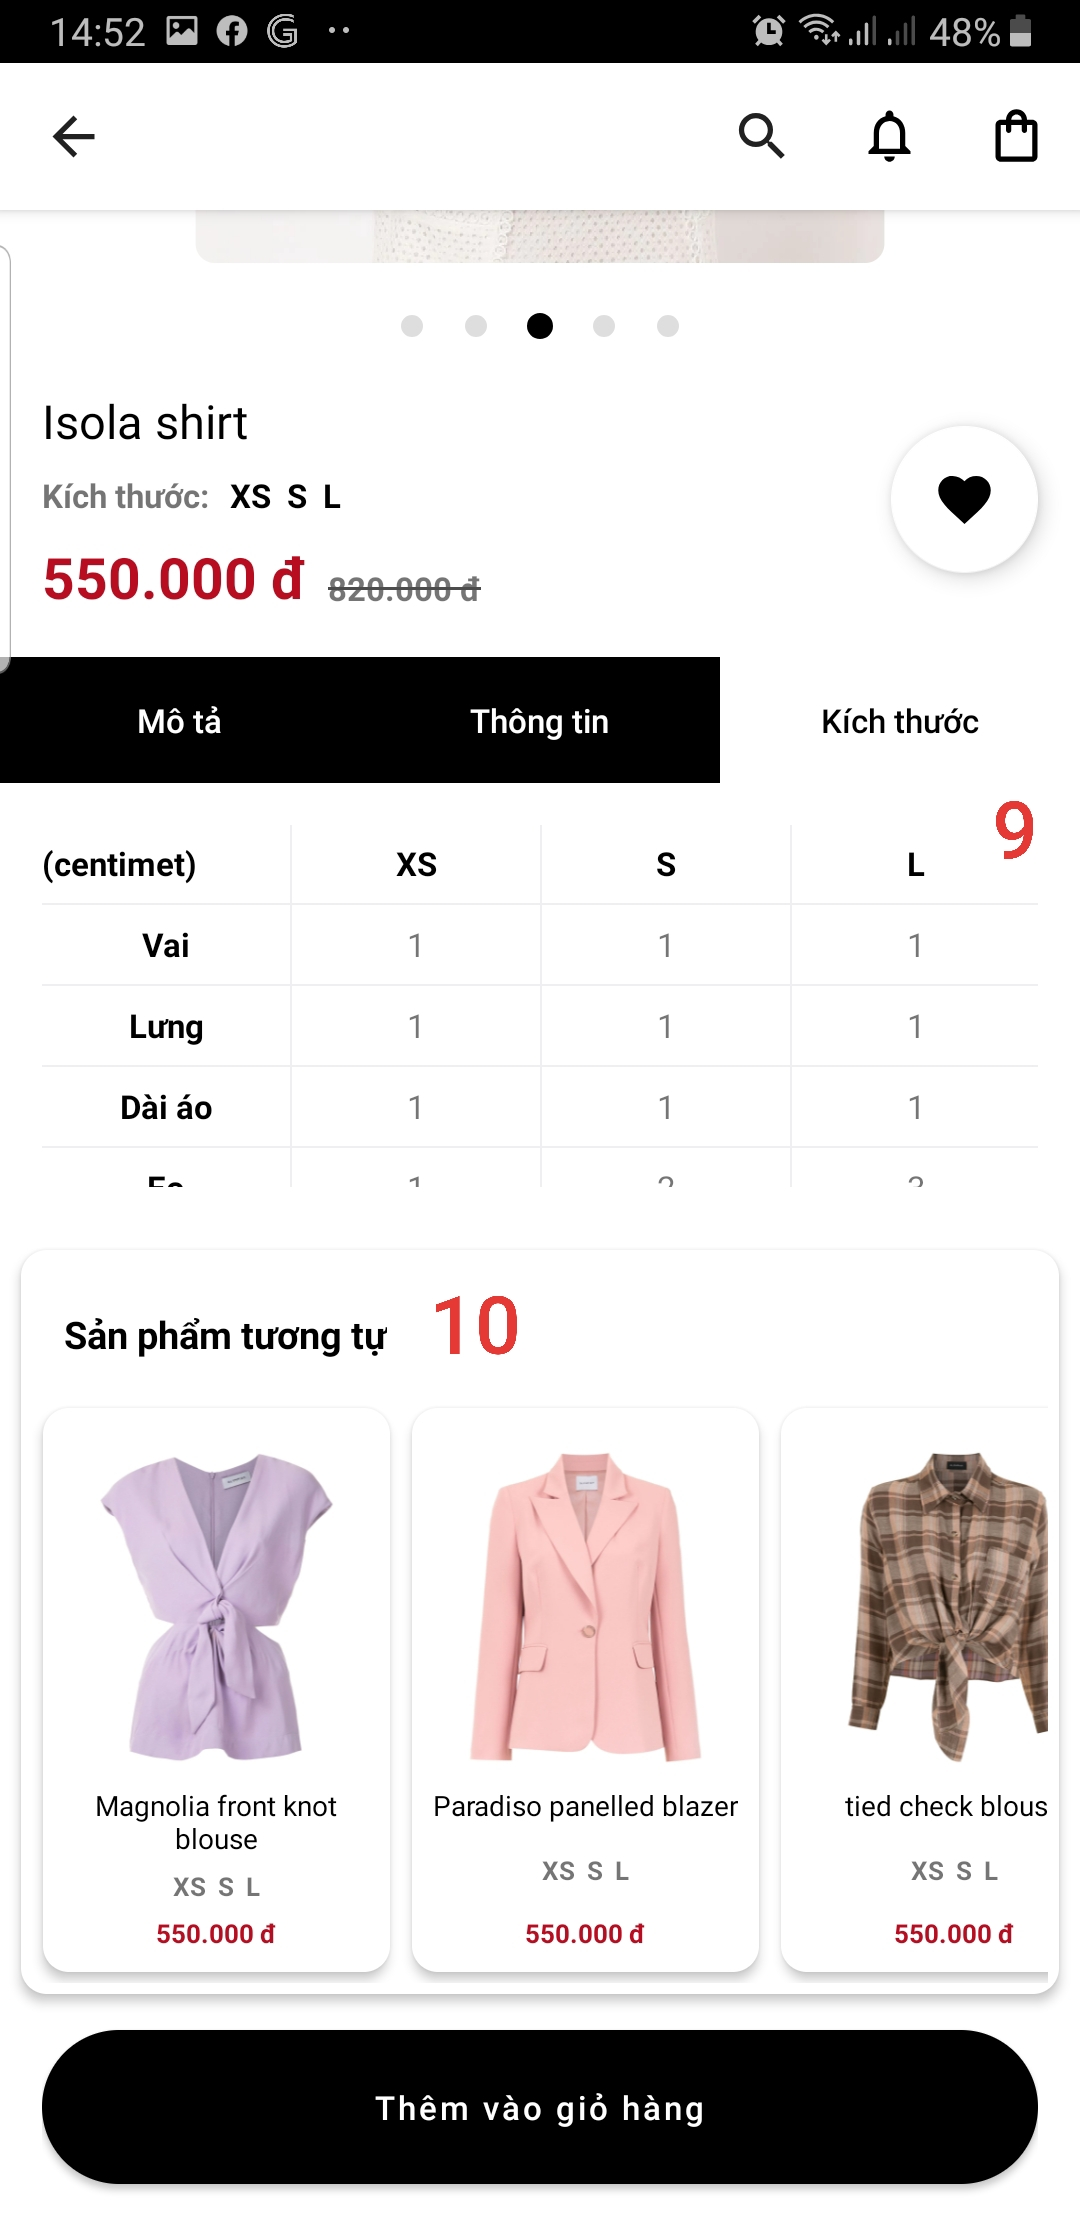
\includegraphics[height=10cm]{images/23.png}
    \caption{Màn hình chi tiết sản phẩm 3}
\end{figure}

\begin{figure}[H]
    \centering
    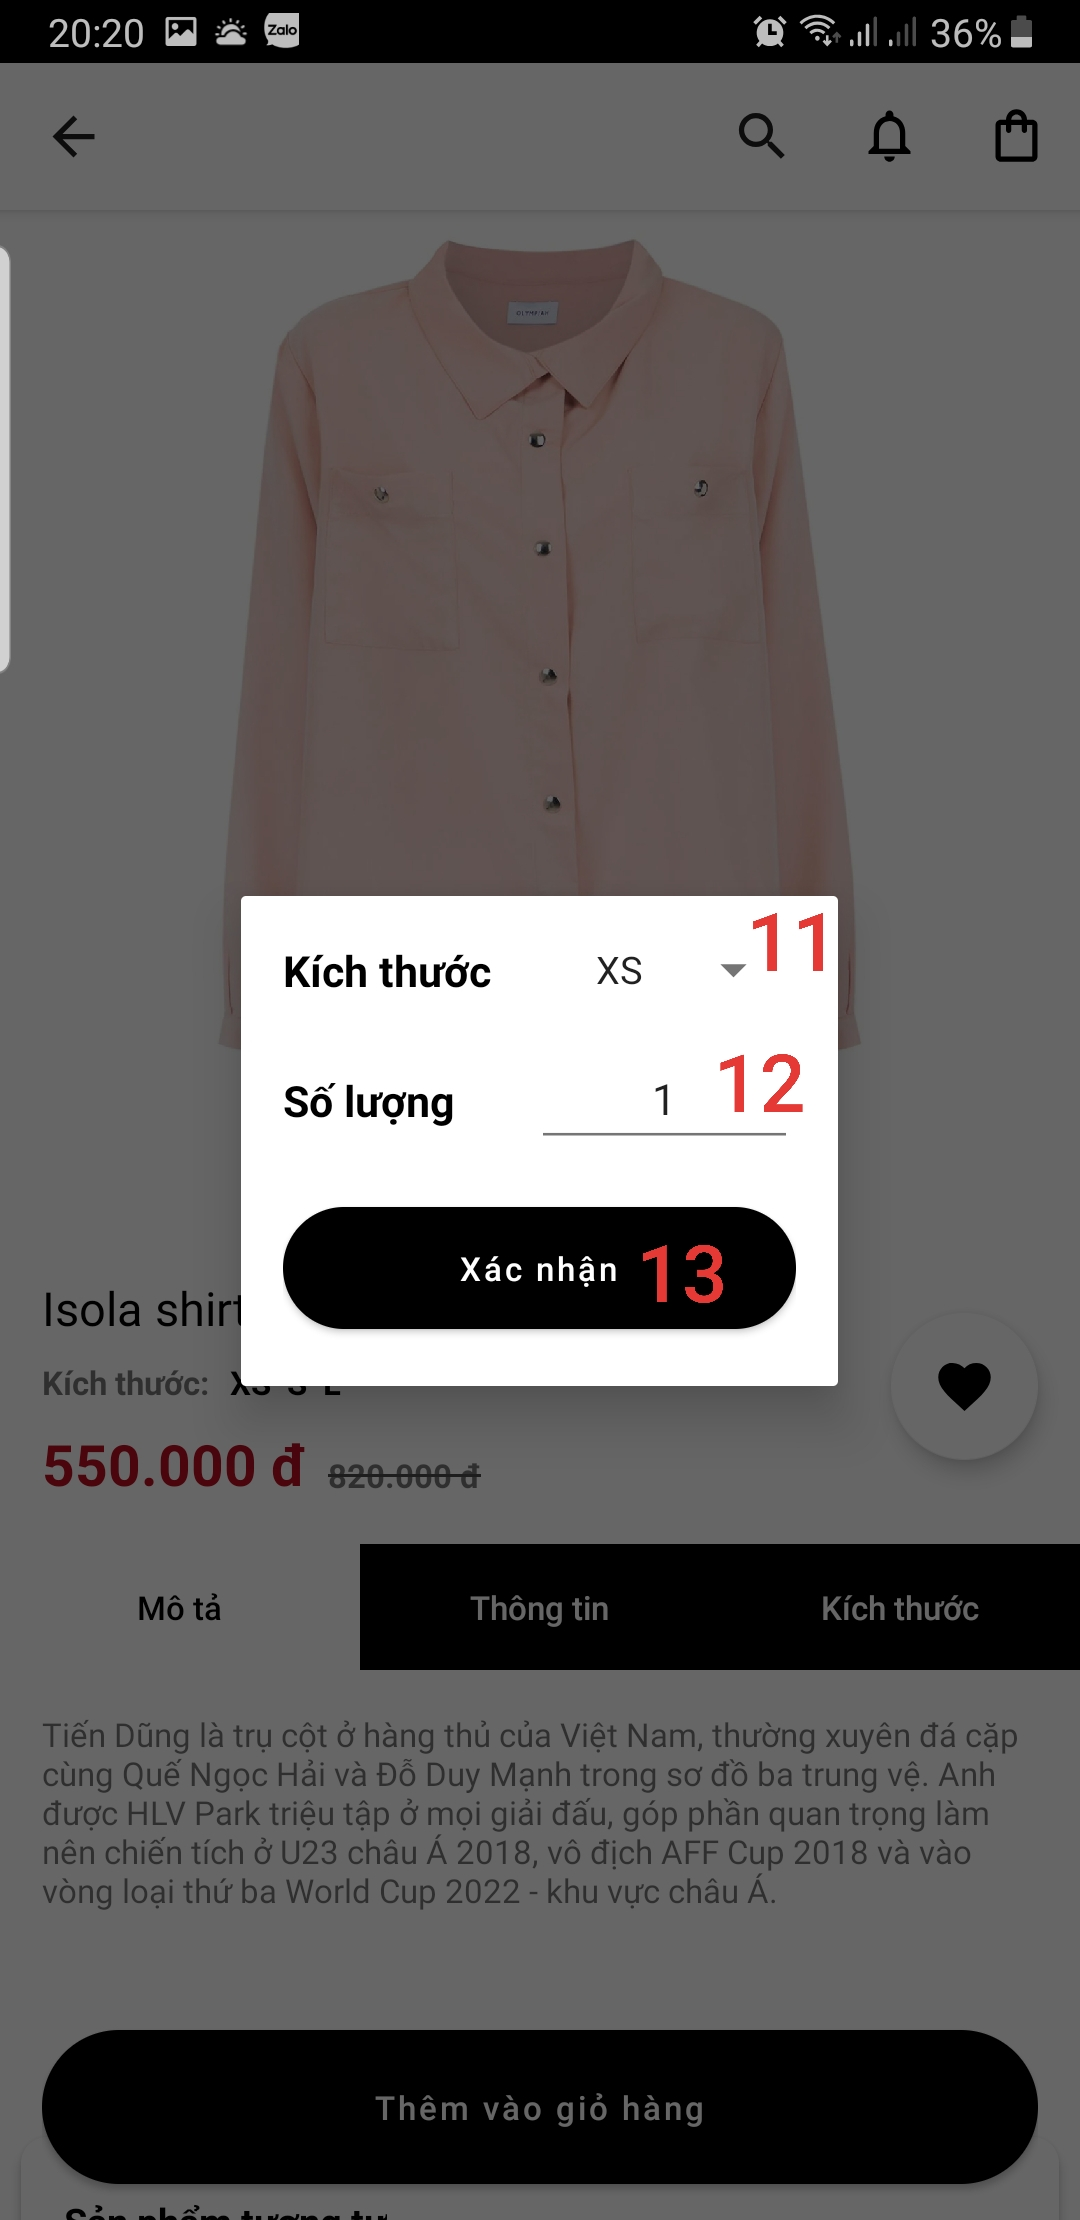
\includegraphics[height=10cm]{images/24.png}
    \caption{Dialog cho phép người dùng chọn size + số lượng sản phẩm thêm vào giỏ hàng}
\end{figure}

\indent \textbf{Các thành phần và chức năng kèm theo trên màn hình}
\begin{itemize}
    \item \textbf{1}: View Pager - hiển thị các hình ảnh của sản phẩm.
    \item \textbf{2}: Floating Action Button - cho phép người dùng nhấn vào để thêm sản phầm vào mục yêu thích. Khi vào màn hình chi tiết một sản phẩm, tuy vào sản phẩm hiện tại có được thêm vào mục yêu thích của người dùng từ trước không mà icon trong button được thay đổi cho phù hợp. Nếu người dùng chưa đăng nhập thì một Toast sẽ hiện lên thông báo cho người dùng biết là chức năng này cần đăng nhập.
    \item \textbf{3}: Các text view - hiển thị thông tin của sản phẩm.
    \item \textbf{4}: As home indicator - quay về fragment trước đó được lưu trong backstack.
    \item \textbf{5}: Menu item Search - nhấn vào để thực hiện chức năng tìm kiếm.
    \item \textbf{6}: Menu item Cart - nhấn vào để đến fragment giỏ hàng.
    \item \textbf{7} + \textbf{9}: TabLayout + View Pager 2 - hiển thị các thông tin thêm về sản phẩm. Bên trong tab "Mô tả" là một Text View, bên trong tab "Thông tin" và "Kích thước" là các GridView.
    \item \textbf{8}: Button - nhấn vào sẽ hiện một Dialog để người dùng có thể chọn size và số lượng sản phẩm để thêm vào giỏ hàng. Nếu người dùng chưa đăng nhập thì một Toast sẽ hiện lên thông báo cho người dùng biết là chức năng này cần đăng nhập.
    \item \textbf{10}: Horizontal Recycler View - hiển thị tám sản phẩm nằm cùng danh mục mới sản phẩm hiện tại, nhấn vào item sẽ đi đến một fragment chi tiết sản phẩm khác tương ứng với sản phẩm đó.
    \item \textbf{11}: Spinner - cho phép người dùng chọn các size của sản phẩm.
    \item \textbf{12}: Text View - để người dùng nhập số lượng sản phẩm cần mua cho size tương ứng.
    \item \textbf{13}: Button - khi click vào sản phẩm sẽ được thêm vào giỏ hàng cùng size và số lượng đã chọn.
\end{itemize}

\subsubsection{Màn hình sản phẩm yêu thích}
Được thực hiện bởi sinh viên 20424008.\\

\indent Chức năng này được truy cập khi người dùng nhấn vào các Hamburger toggle, sau đó thông qua navigation view mà người dùng có thể truy cập vào màn hình này (xem lại hình 14 ở mục 2.3.1).\\

\indent Người dùng chỉ có thể truy cập vào màn hình này khi đã đăng nhập, nếu chưa đăng nhập thì một Toast sẽ hiện lên yêu cầu người dùng đăng nhập để sử dụng tính năng này. Dưới đây là hình chụp của màn hình này.

\begin{figure}[H]
    \centering
    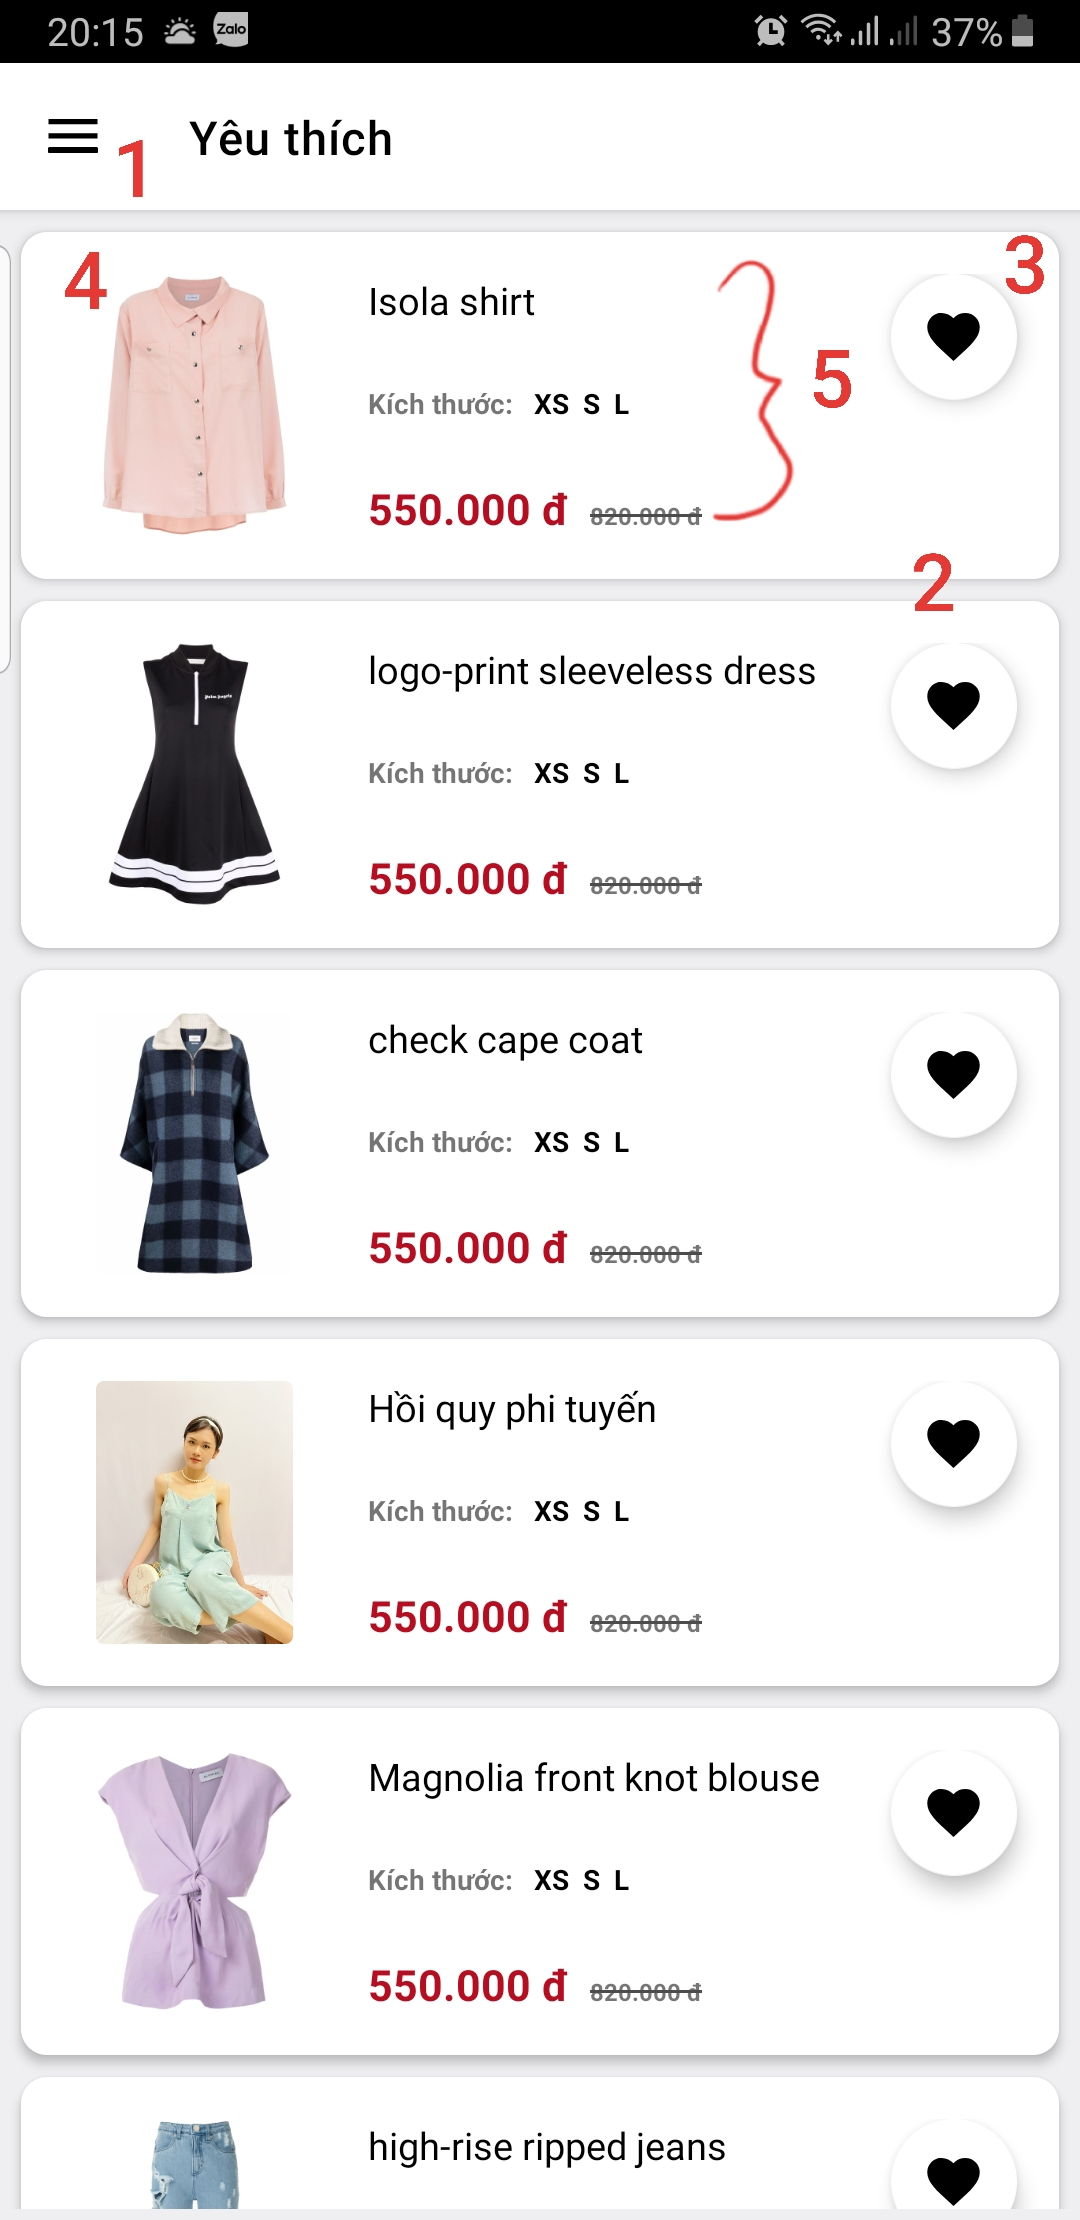
\includegraphics[height=10cm]{images/25.png}
    \caption{Màn hình sản phẩm yêu thích}
\end{figure}

\indent \textbf{Các thành phần và chức năng kèm theo trên màn hình}
\begin{itemize}
    \item \textbf{1}: Hamburger toggle - dùng để truy cập vào navigation view.
    \item \textbf{2}: Vertical Recycler View - hiển thị các sản phẩm mà người dùng đã thêm vào mục yêu thích của mình.
    \item \textbf{3}: Floating Action Button - người dùng có thể nhấn vào để xóa sản phẩm khỏi mục yêu thích. Tuy nhiên để tránh người dùng nhấn nhầm, ứng dụng không xóa ngay mà chỉ chuyển icon của button này đi, cho đến khi fragment này rơi vào \texttt{onPause} thì nó mới thực sự được xóa khỏi mục yêu thích của người dùng và Firestore được cập nhật.
    \item \textbf{4}: Image view - hiển thị hình ảnh của sản phẩm, nếu người dùng nhấn vào thì sẽ đưa người dùng đến trang chi tiết sản phẩm của sản phẩm đó.
    \item \textbf{5}: Các Text View - hiển thị các thông tin cơ bản của sản phẩm.
\end{itemize}

\subsubsection{Chức năng tìm kiếm sản phẩm}
Được thực hiện bởi sinh viên 20424008.\\

\indent Chức năng này được sử dụng ở các màn hình nằm ở các mục 2.3.1, 2.3.2, 2.3.3 và 2.3.4. Cho phép người dùng tìm kiếm theo từ khóa dựa trên tên của sản phẩm. Dưới đây là hình chụp từ màn hình này.

\begin{figure}[H]
    \centering
    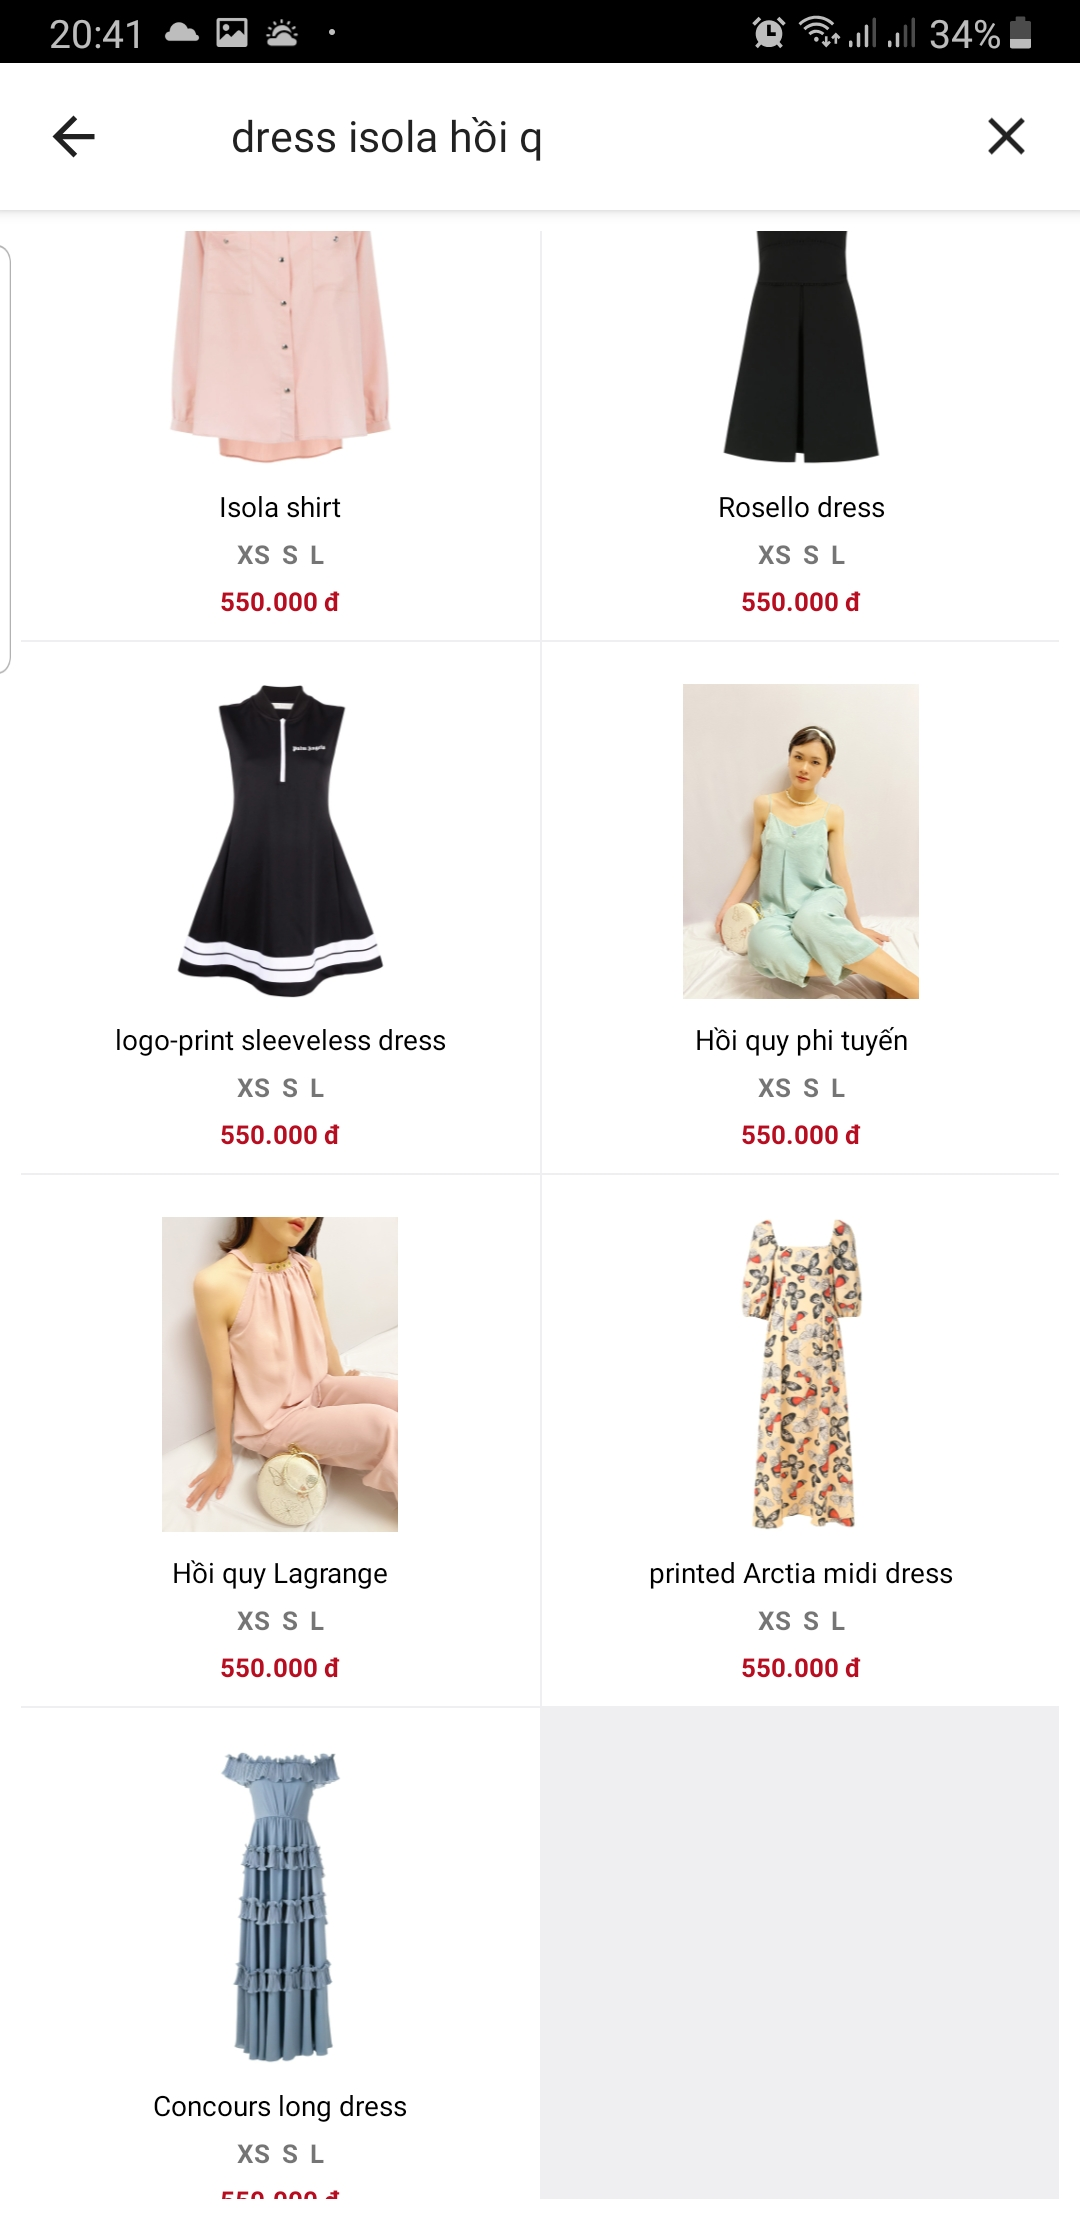
\includegraphics[height=10cm]{images/26.png}
    \caption{Màn hình sản phẩm yêu thích}
\end{figure}

\indent \textbf{Các thành phần và chức năng kèm theo trên màn hình}
\begin{itemize}
    \item Khi người dùng nhấn vào bất kì một menu item search nào, một search box như hình trên sẽ hiển thị ra, đồng thời người dùng sẽ được đưa đến một fragment khác, nơi các sản phẩm được tìm kiểm sẽ hiển thị dưới dạng một GridView.
    \item Ở đây, em tìm kiếm các sản phẩm dựa vào ba từ khóa là \textsf{dress}, \textsf{isola} và \textsf{hồi}, thì toàn bộ các sản phẩm được tìm ra bên dưới đều có tên chứa ít nhất một từ mà người dùng nhập vào.
\end{itemize}

\subsubsection{Màn hình giỏ hàng}
Được thực hiện bởi sinh viên 20424013.\\

\indent Người dùng chỉ có thể truy cập vào màn hình này khi đã đăng nhập, nếu không một Toast sẽ hiện lên thông báo cho người dùng cần đăng nhập để sử dụng tính năng này.\\

\indent Màn hình này có thể được truy cập thông qua navigation view khi người dùng nhấn vào Hamburger toggle hoặc thông qua menu item cart. Dưới đây là hình chụp màn hình này.

\begin{figure}[H]
    \centering
    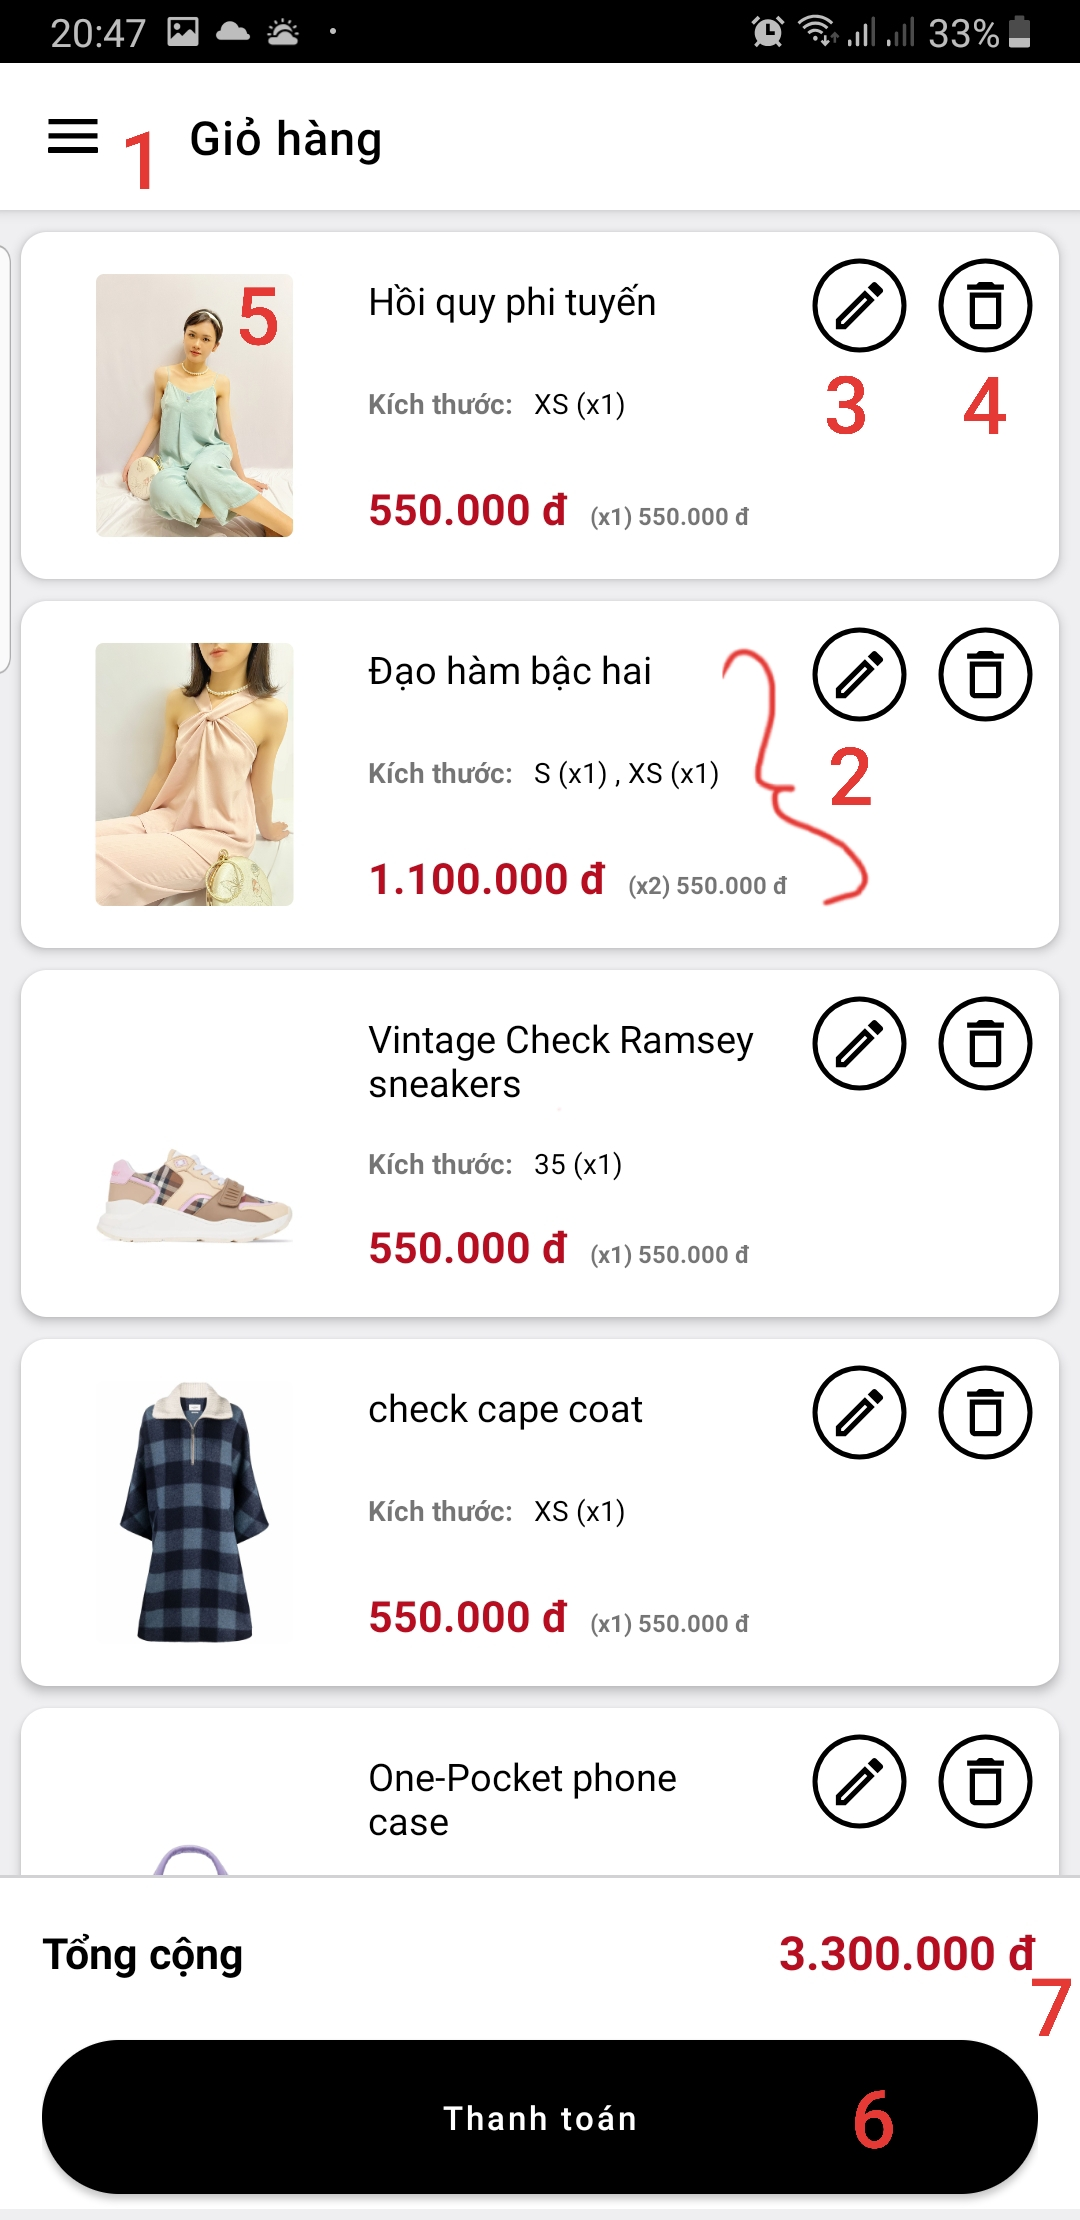
\includegraphics[height=10cm]{images/27.png}
    \caption{Màn hình giỏ hàng}
\end{figure}

\begin{figure}[H]
    \centering
    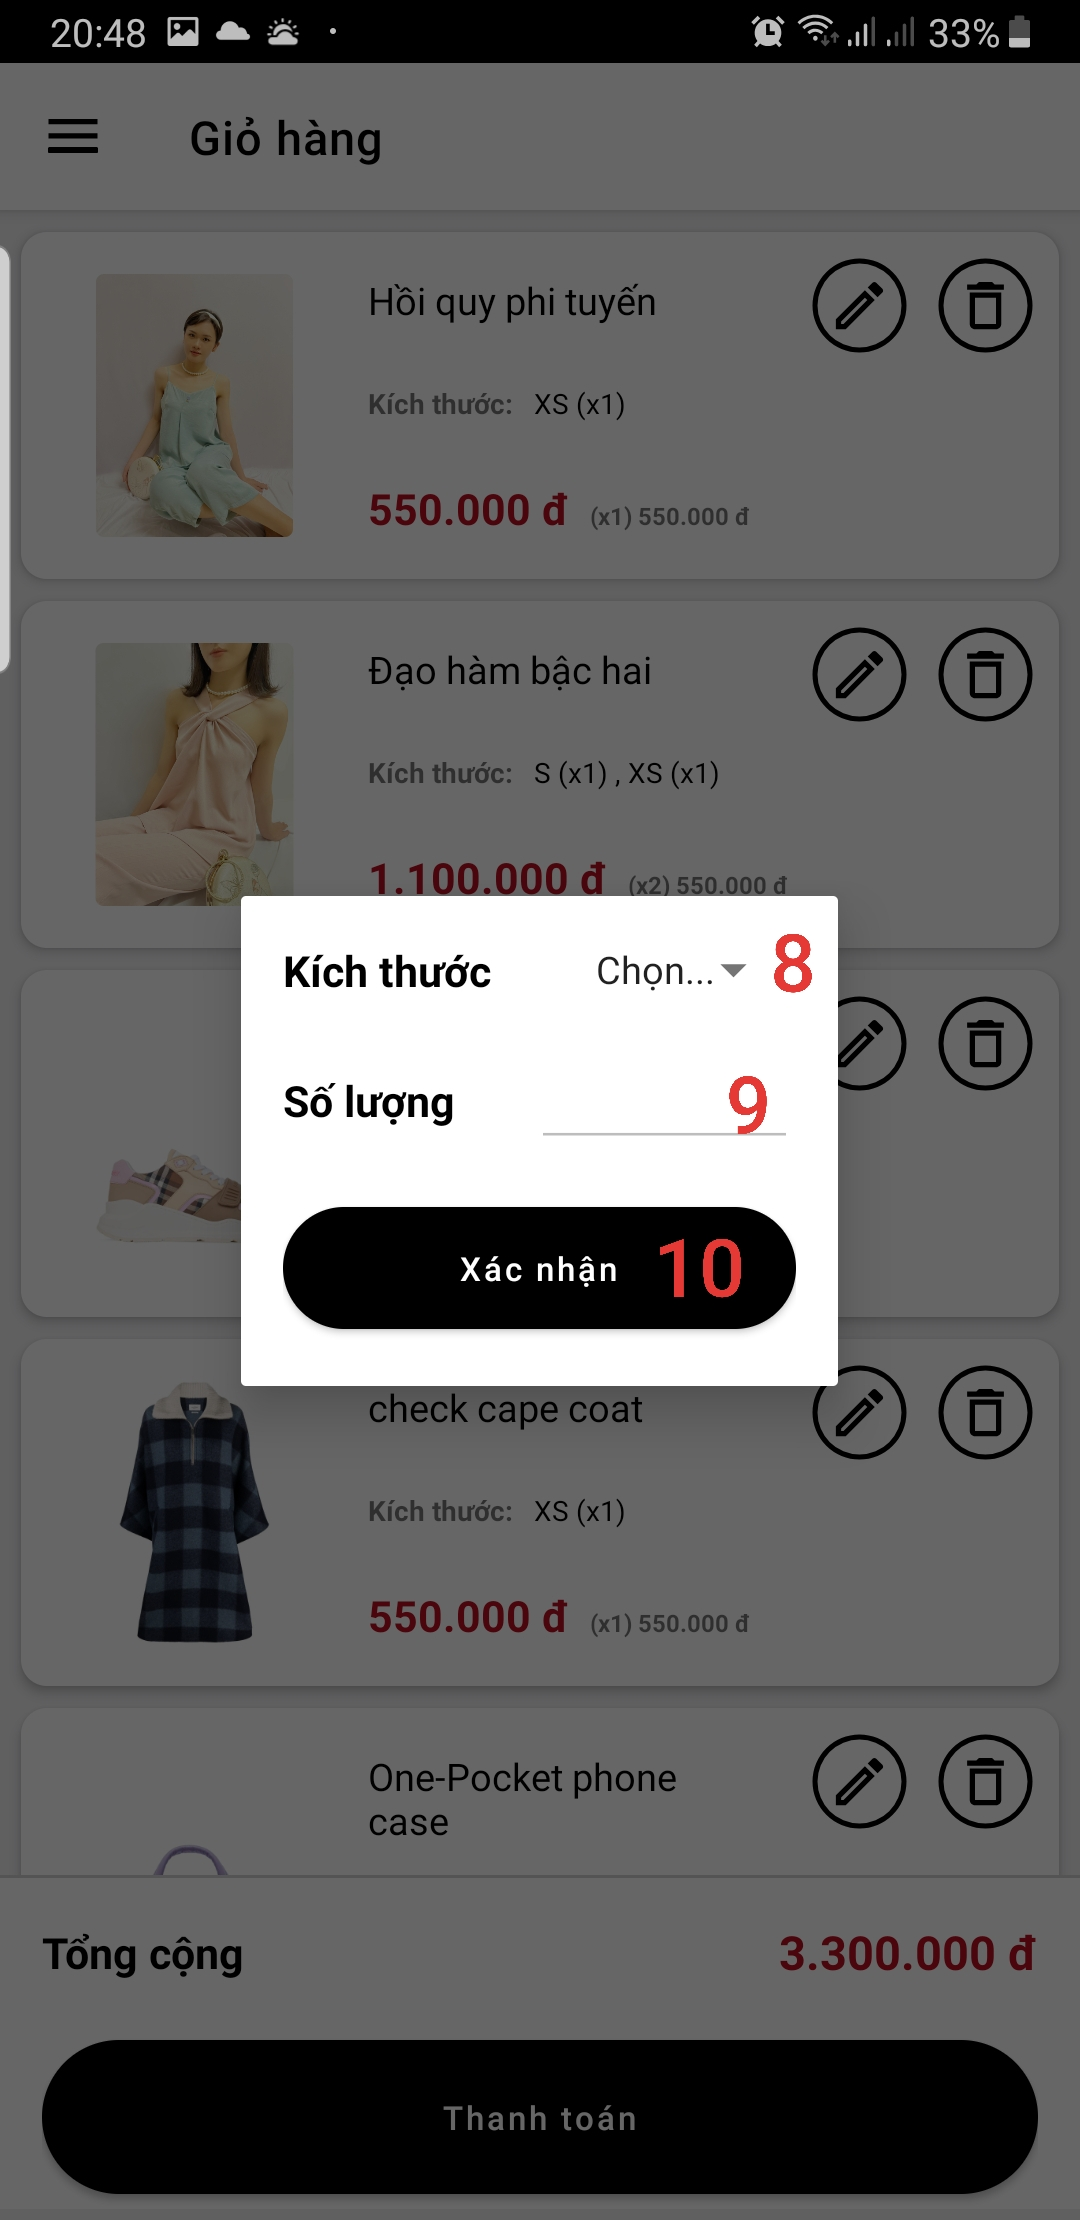
\includegraphics[height=10cm]{images/28.png}
    \caption{Màn hình giỏ hàng - dialog chỉnh sửa sản phẩm}
\end{figure}

\begin{figure}[H]
    \centering
    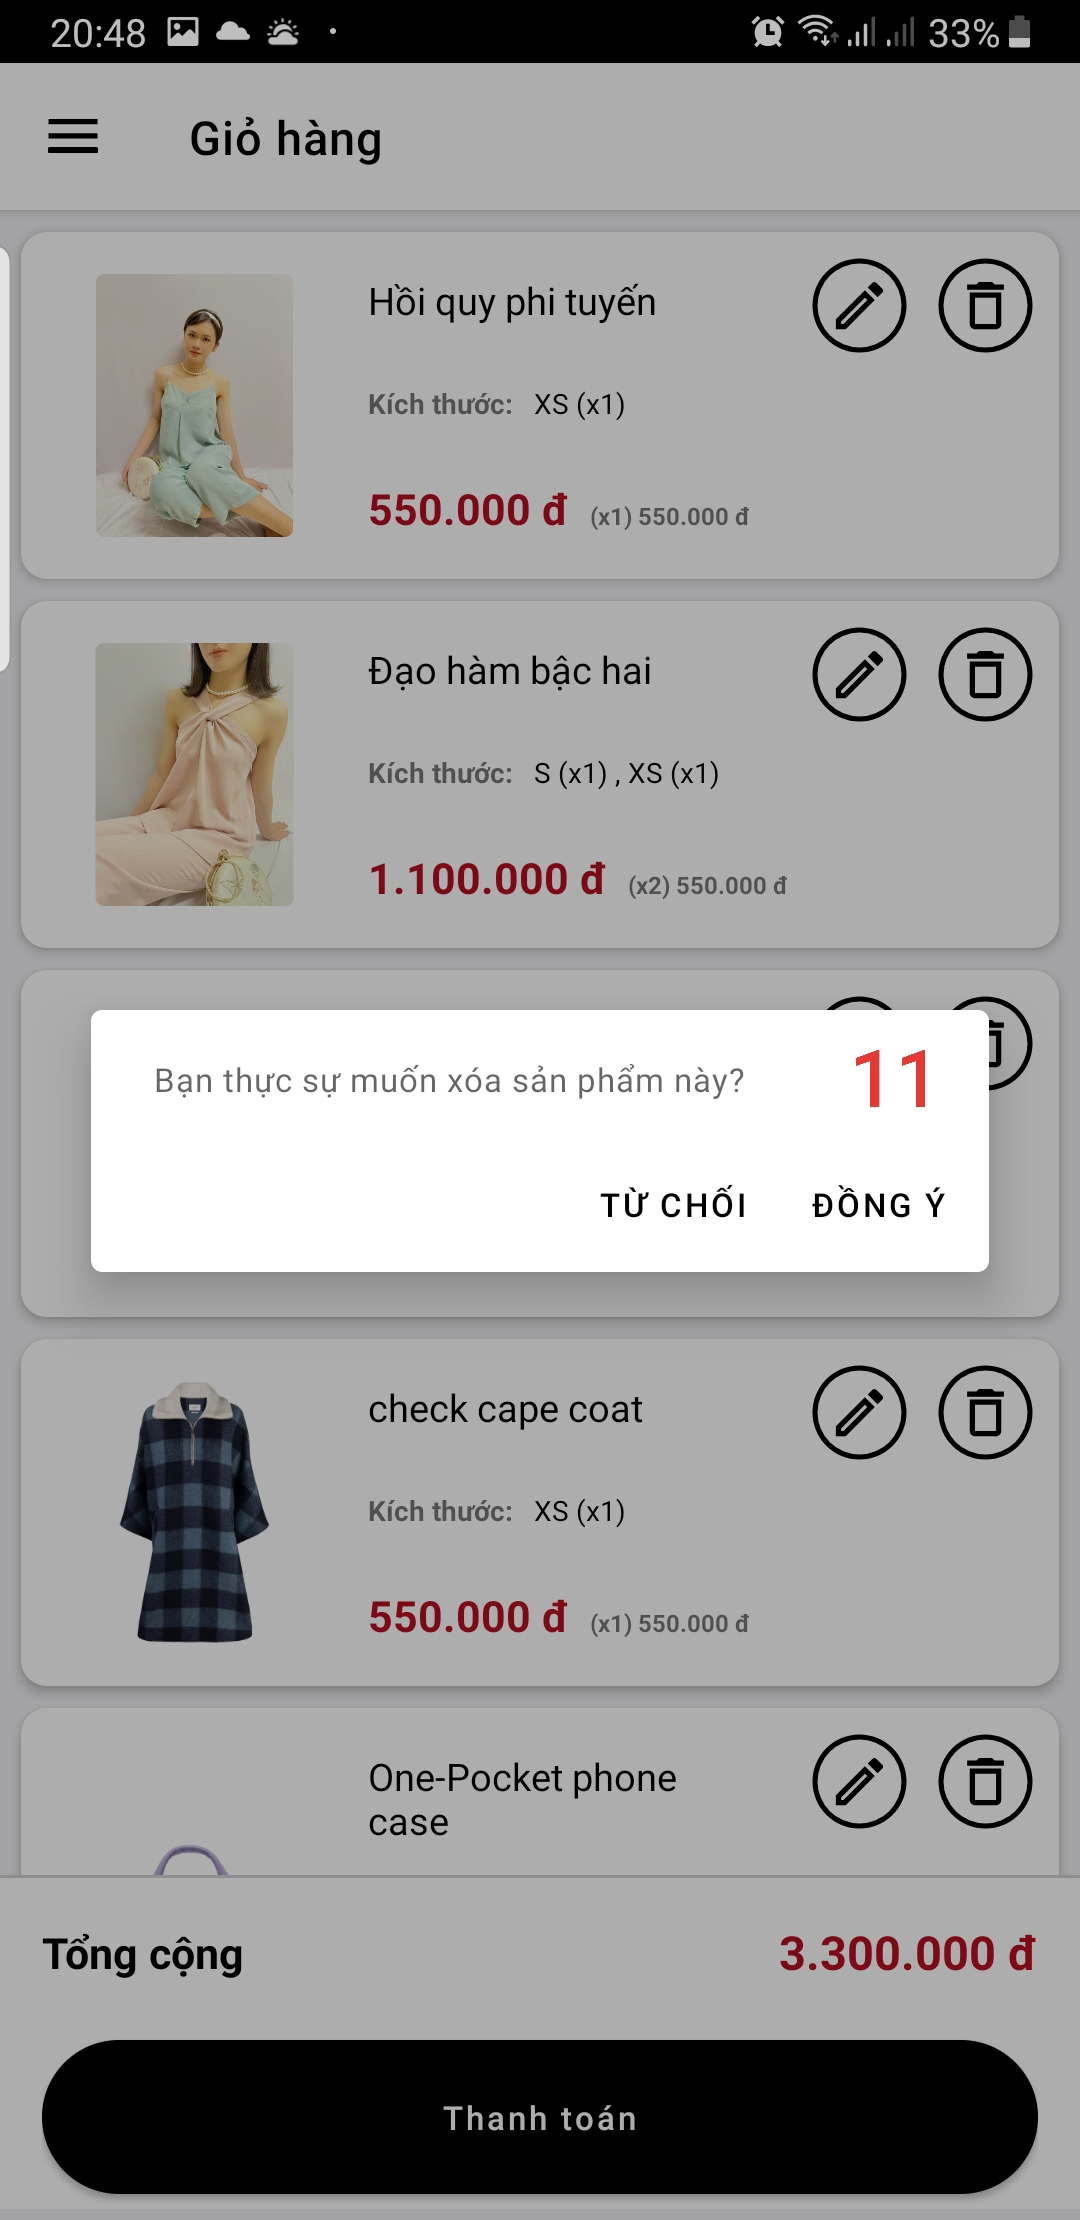
\includegraphics[height=10cm]{images/29.png}
    \caption{Màn hình giỏ hàng - Alert Dialog cảnh báo sản phẩm sẽ bị xóa}
\end{figure}

\newpage
\indent \textbf{Các thành phần và chức năng kèm theo trên màn hình}
\begin{itemize}
    \item \textbf{1}: Hamburger toggle - để người dùng truy cập vào navigation view.
    \item \textbf{2}: Các Text view - thể hiện tên sản phẩm, các size và số lượng sản phẩm được đặt với size tương ứng, tổng tiền cho sản phẩm đó.
    \item \textbf{3}: Image button - nhấn vào cho phép người dùng chỉnh sửa sản phẩm tương ứng.
    \item \textbf{4}: Image button - nhấn vào một alert dialog hiện ra cảnh báo cho người dùng rằng họ có chắc chắn muốn xóa sản phẩm này khỏi giỏ hàng hay không.
    \item \textbf{5}: Image view - nhấn vào sẽ đi đến màn hình chi tiết sản phẩm của sản phẩm đó để thêm vào yêu thích, đặt size khác.
    \item \textbf{6}: Button - nhấn vào để đi đến màn hình thanh toán.
    \item \textbf{7}: Text View - thể hiện tổng giá trị của giỏ hàng.
    \item \textbf{8}: Spinner - nằm trong dialog khi người dùng nhấn vào thành phần \textbf{3}, cho phép người dùng chọn size cần chỉnh số lượng.
    \item \textbf{9}: Text input - để người dùng thay đổi số lượng của sản phẩm theo size tương ứng.
    \item \textbf{10}: Button - khi nhấn vào thì size và số lượng hiện tại sẽ được cập nhật lại vào giỏ hàng.
    \item \textbf{11}: Alert Dialog - cảnh báo khi người dùng nhấn vào thành phần \textbf{4}, để xác nhận người dùng có thực sự muốn xóa sản phẩm khỏi giỏ hàng hay không. Nếu người dùng chọn "Đồng ý" thì sản phẩm sẽ bị xóa khỏi đơn hàng và đơn hàng được cập nhật lại.
\end{itemize}

\subsubsection{Màn hình thanh toán}
Được thực hiện bởi sinh viên 20424013.\\

\indent Màn hình này được truy cập khi người dùng nhấn vào thành phần \textbf{6} trên màn hình giỏ hàng (xem hình 27 mục 2.3.7). Cho phép người dùng thực hiện thanh toán cho đơn hàng. Dưới đây là hình chụp màn hình này.

\begin{figure}[H]
    \centering
    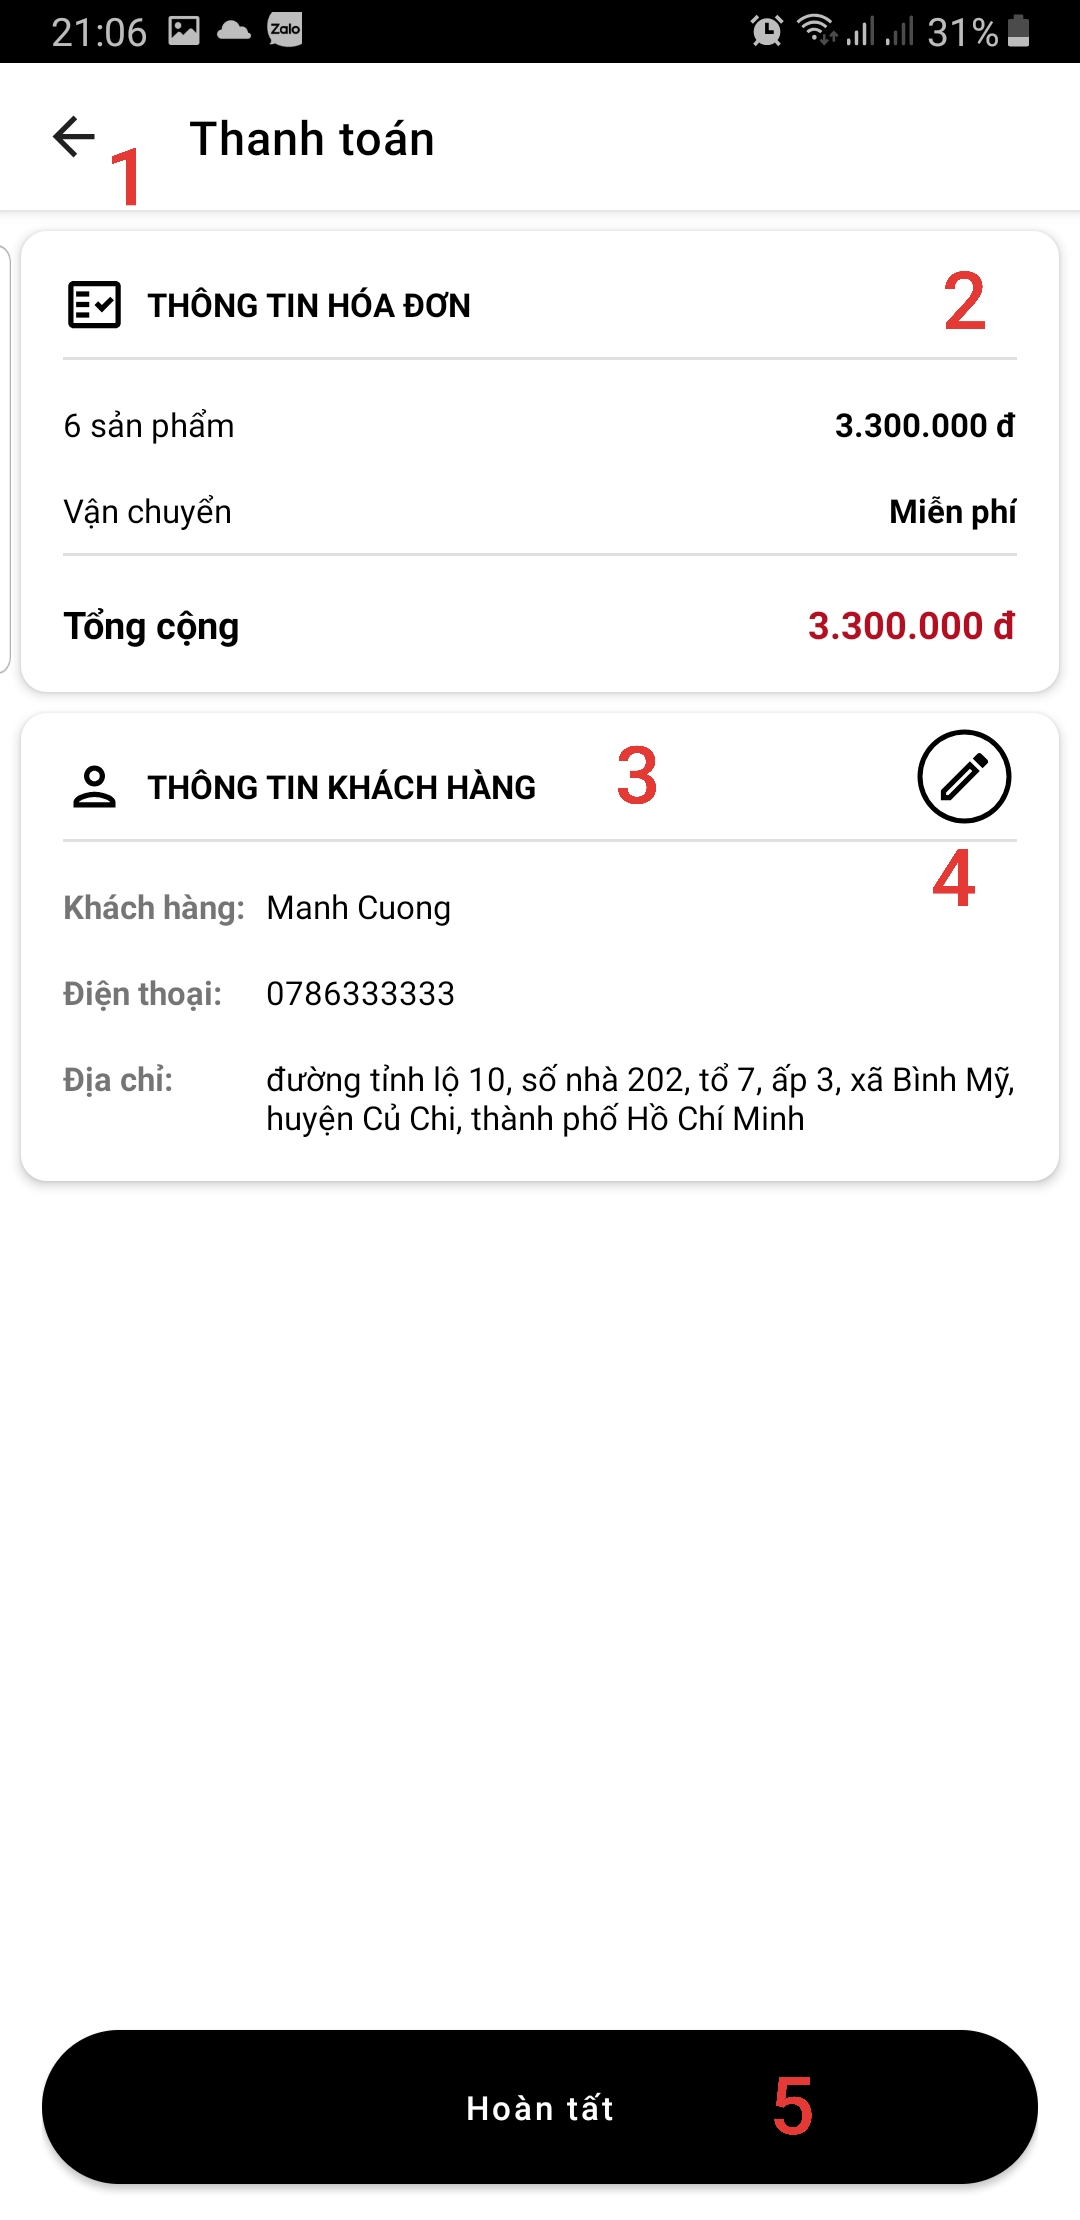
\includegraphics[height=10cm]{images/30.png}
    \caption{Màn hình thanh toán}
\end{figure}

\begin{figure}[H]
    \centering
    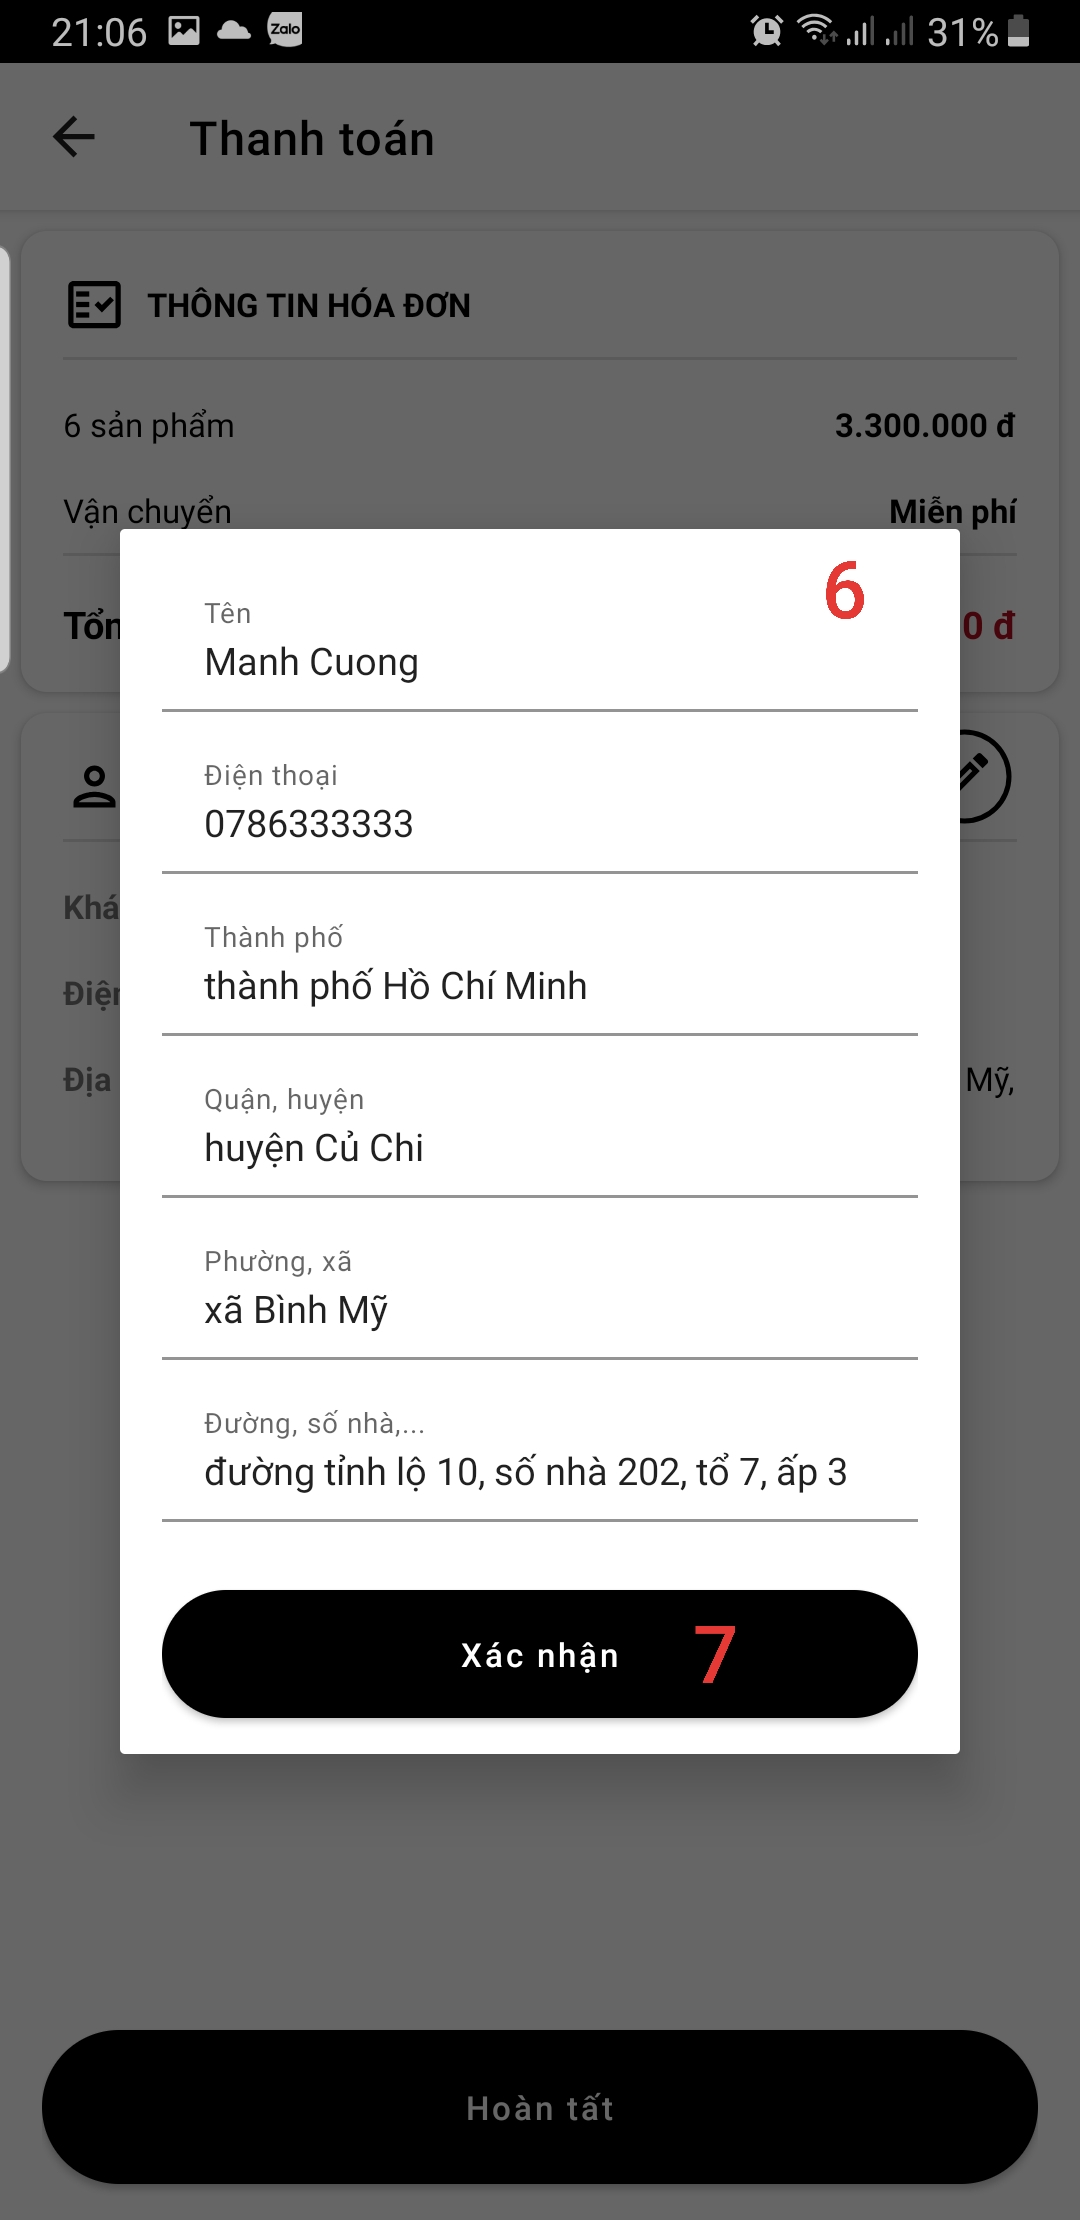
\includegraphics[height=10cm]{images/31.png}
    \caption{Màn hình thanh toán - chỉnh sửa địa chỉ giao hàng}
\end{figure}

\begin{figure}[H]
    \centering
    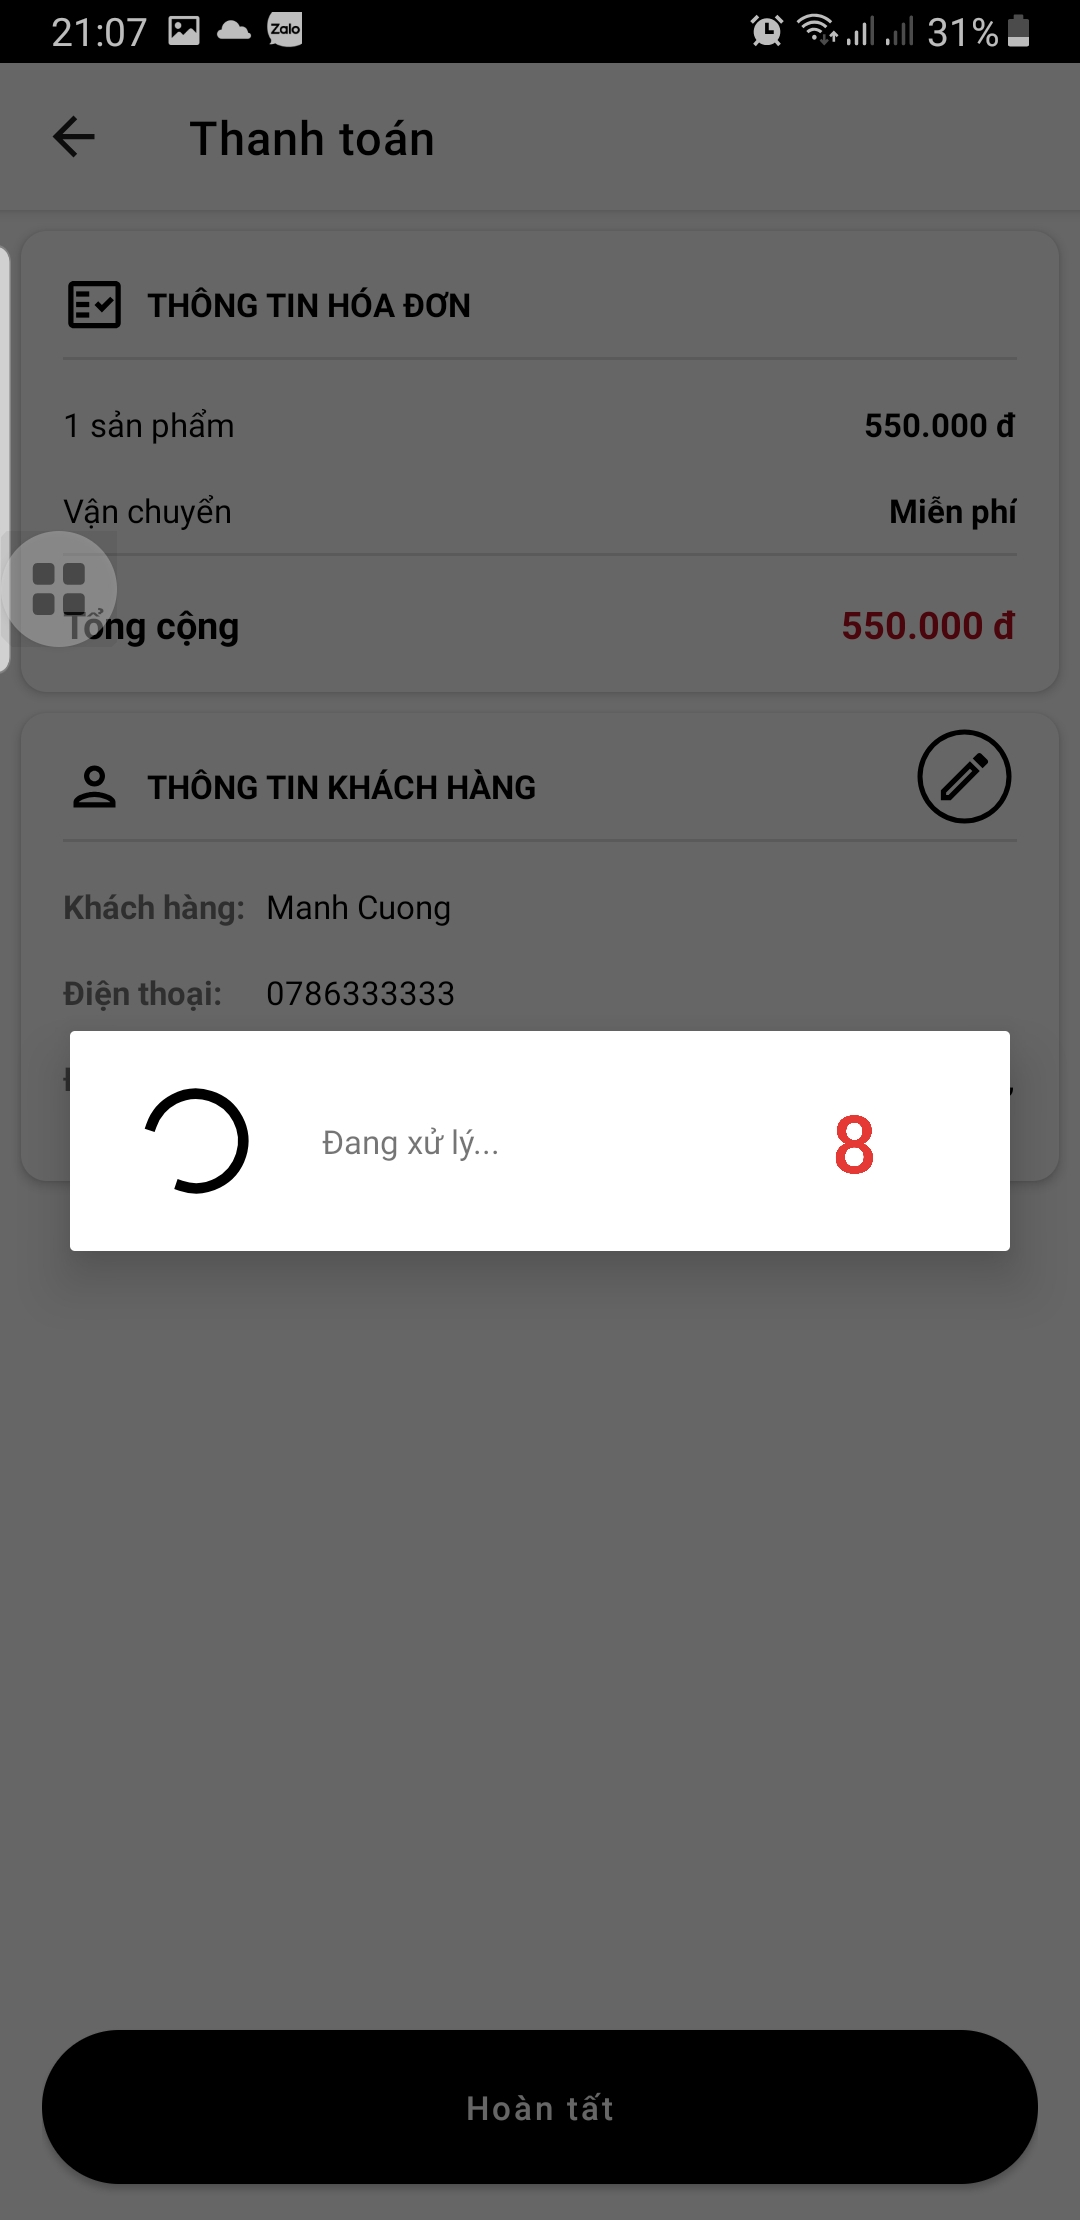
\includegraphics[height=10cm]{images/32.png}
    \caption{Màn hình thanh toán - progress dialog}
\end{figure}

\begin{figure}[H]
    \centering
    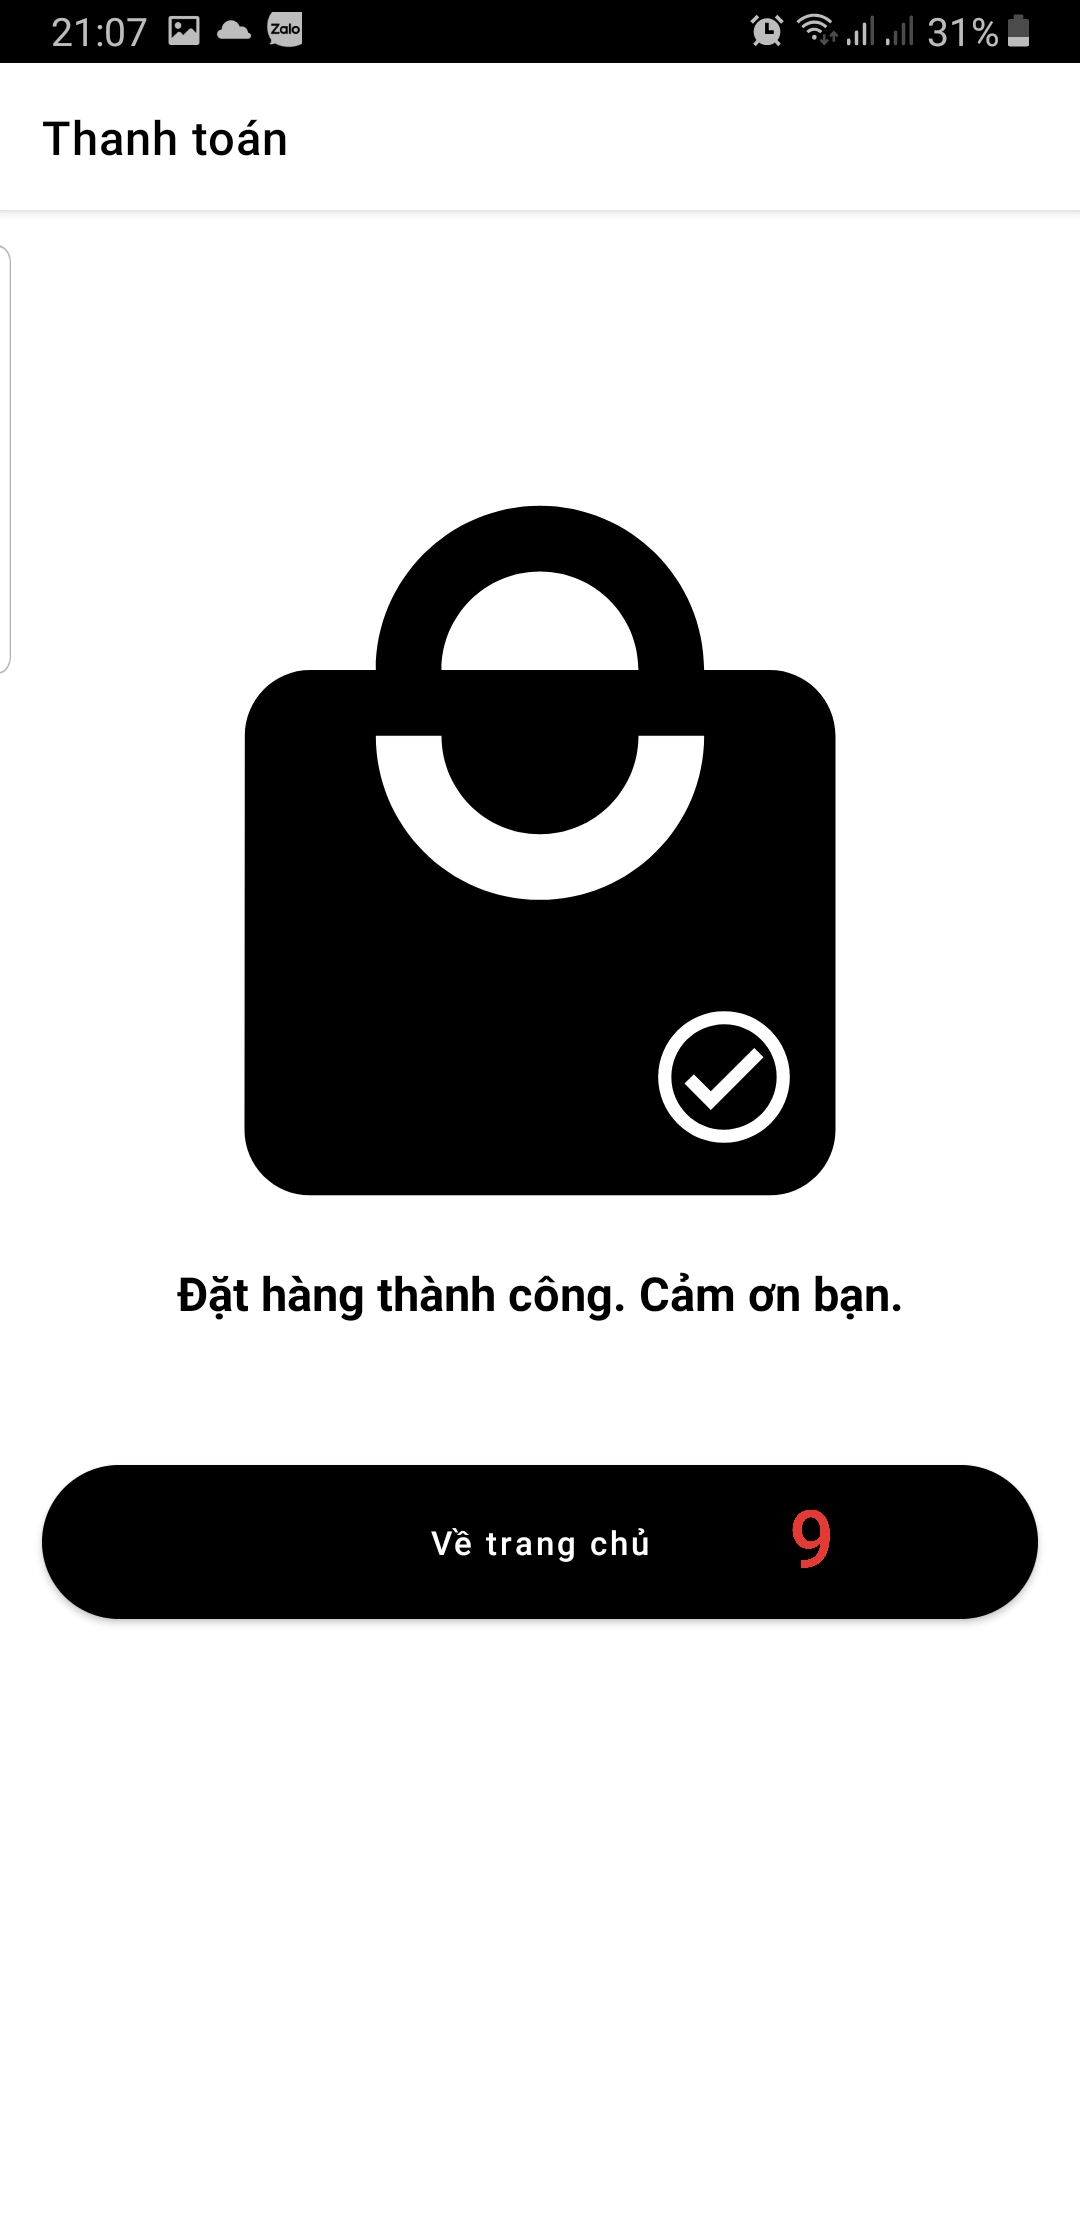
\includegraphics[height=10cm]{images/33.png}
    \caption{Màn hình thanh toán - đặt hàng thành công}
\end{figure}

\newpage
\indent \textbf{Các thành phần và chức năng kèm theo trên màn hình}
\begin{itemize}
    \item \textbf{1}: As home indicator - nhấn vào để quay về màn hình giỏ hàng.
    \item \textbf{2}: Các text view - thể hiện số sản phẩm của hóa đơn, tổng tiền, tiền vận chuyển.
    \item \textbf{3}: Các text view - hiển thị địa chỉ giao hàng mặc định (nếu người dùng đã thiết lập trong fragment tài khoản, nhóm sẽ trình bày sau). Nếu chưa đăng nhập thì các trường này là rỗng.
    \item \textbf{4}: Image Button - cho phép người dùng thay đổi địa chỉ giao hàng.
    \item \textbf{5}: Button - xác nhận thanh toán, chỉ có thể click nếu toàn bộ các trường trong thành phần \textbf{3} đã được nhập, nếu không thể hiện Toast cảnh báo người dùng chưa nhập đầy đủ thông tin.
    \item \textbf{6}: Dialog - cho phép người dùng thay đổi địa chỉ giao hàng.
    \item \textbf{7}: Button - cập nhập lại địa chỉ giao hàng mới.
    \item \textbf{8}: Progress Dialog - hiển thị khi người dùng nhấn vào thành phần \textbf{7}, lúc này ứng dụng đang ghi dữ liệu vào Firestore, dialog này sẽ tắt khi Firestore trả về kết quả.
    \item \textbf{9}: Nếu đơn hàng được đặt thành công thì một màn hình như hình 33 sẽ hiển thị đi kèm là button để quay về trang chính của ứng dụng ở mục 2.3.1.
\end{itemize}

\subsubsection{Màn hình lịch sử đơn hàng}
Được thực hiện bởi sinh viên 20424013.\\

\indent Màn hình này được truy cập thông qua navigation view và chỉ khi người dùng đã đăng nhập, nếu không thì một Toast sẽ thông báo yêu cầu người dùng đăng nhập.

\indent Màn hình này giúp lưu lại lịch sử của đơn hàng của người dùng. Dưới đây là hình chụp của màn hình này.

\begin{figure}[H]
    \centering
    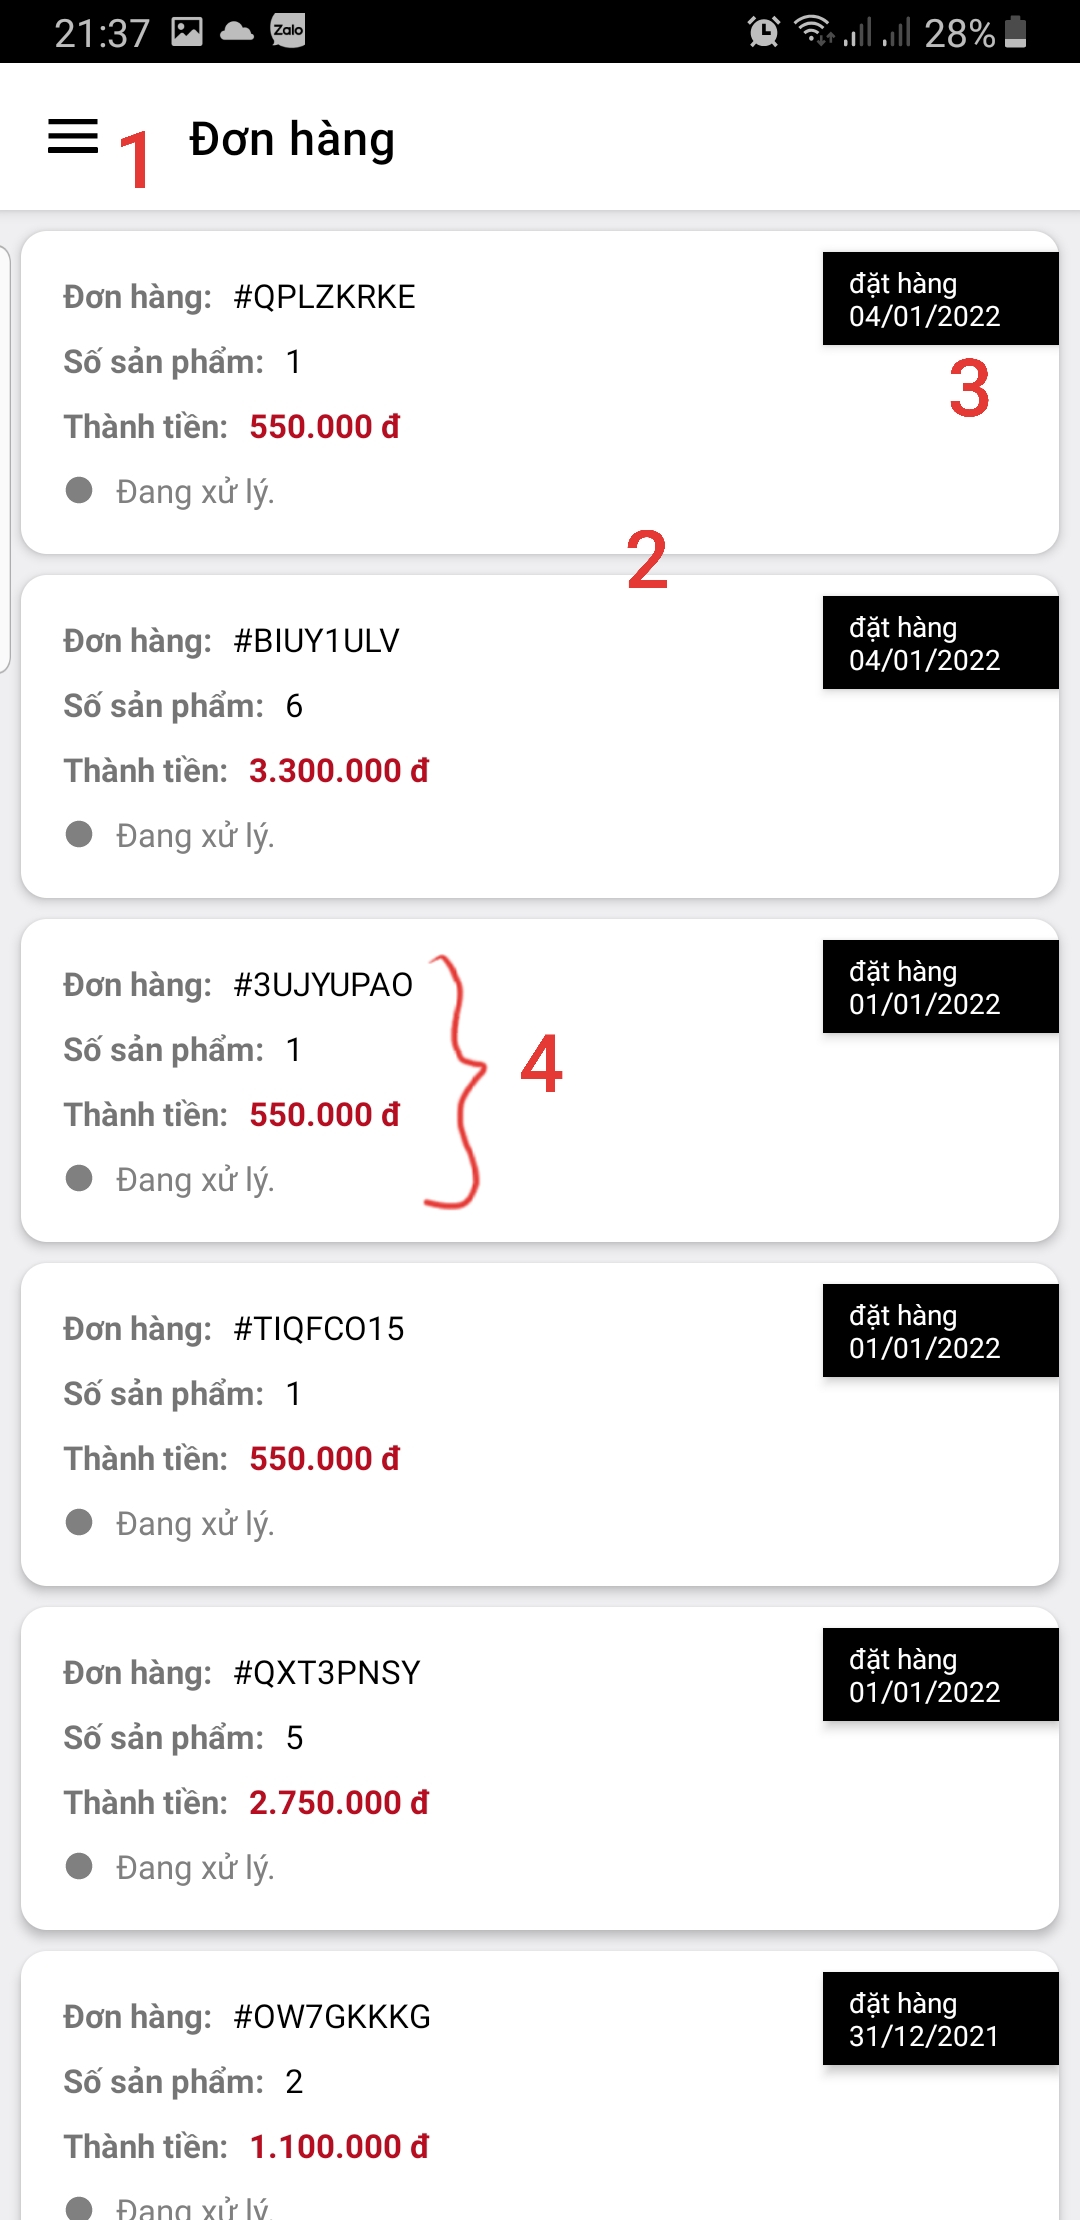
\includegraphics[height=10cm]{images/36.png}
    \caption{Màn hình lịch sử đơn hàng}
\end{figure}

\indent \textbf{Các thành phần và chức năng kèm theo trên màn hình}
\begin{itemize}
    \item \textbf{1}: Hamburger toggle - để truy cập vào navigation view.
    \item \textbf{2}: Vertical Recycler View - hiển thị các đơn hàng của người dùng. Khi người dùng nhấn vào một item thì sẽ được đưa đến màn hình chi tiết đơn hàng sẽ được trình bày ở mục 2.3.10.
    \item \textbf{3}: Linear Layout + Text View - hiển thị ngày đặt hàng của đơn hàng đó.
    \item \textbf{4}: Các Text View - hiển thị thông tin của đơn hàng, bao gồm mã đơn hàng, số sản phẩm, tổng tiền và trạng thái đơn hàng.
\end{itemize}

\subsubsection{Màn hình chi tiết đơn hàng}
Được thực hiện bởi sinh viên 20424013.\\

\indent Màn hình này thể hiện chi tiết của một đơn hàng, được truy cập khi người dùng nhấn vào một item của Vertical Recycler View ở màn hình lịch sử đơn hàng ở mục 2.3.9. Dưới đây là hình chụp của màn hình này.

\begin{figure}[H]
    \centering
    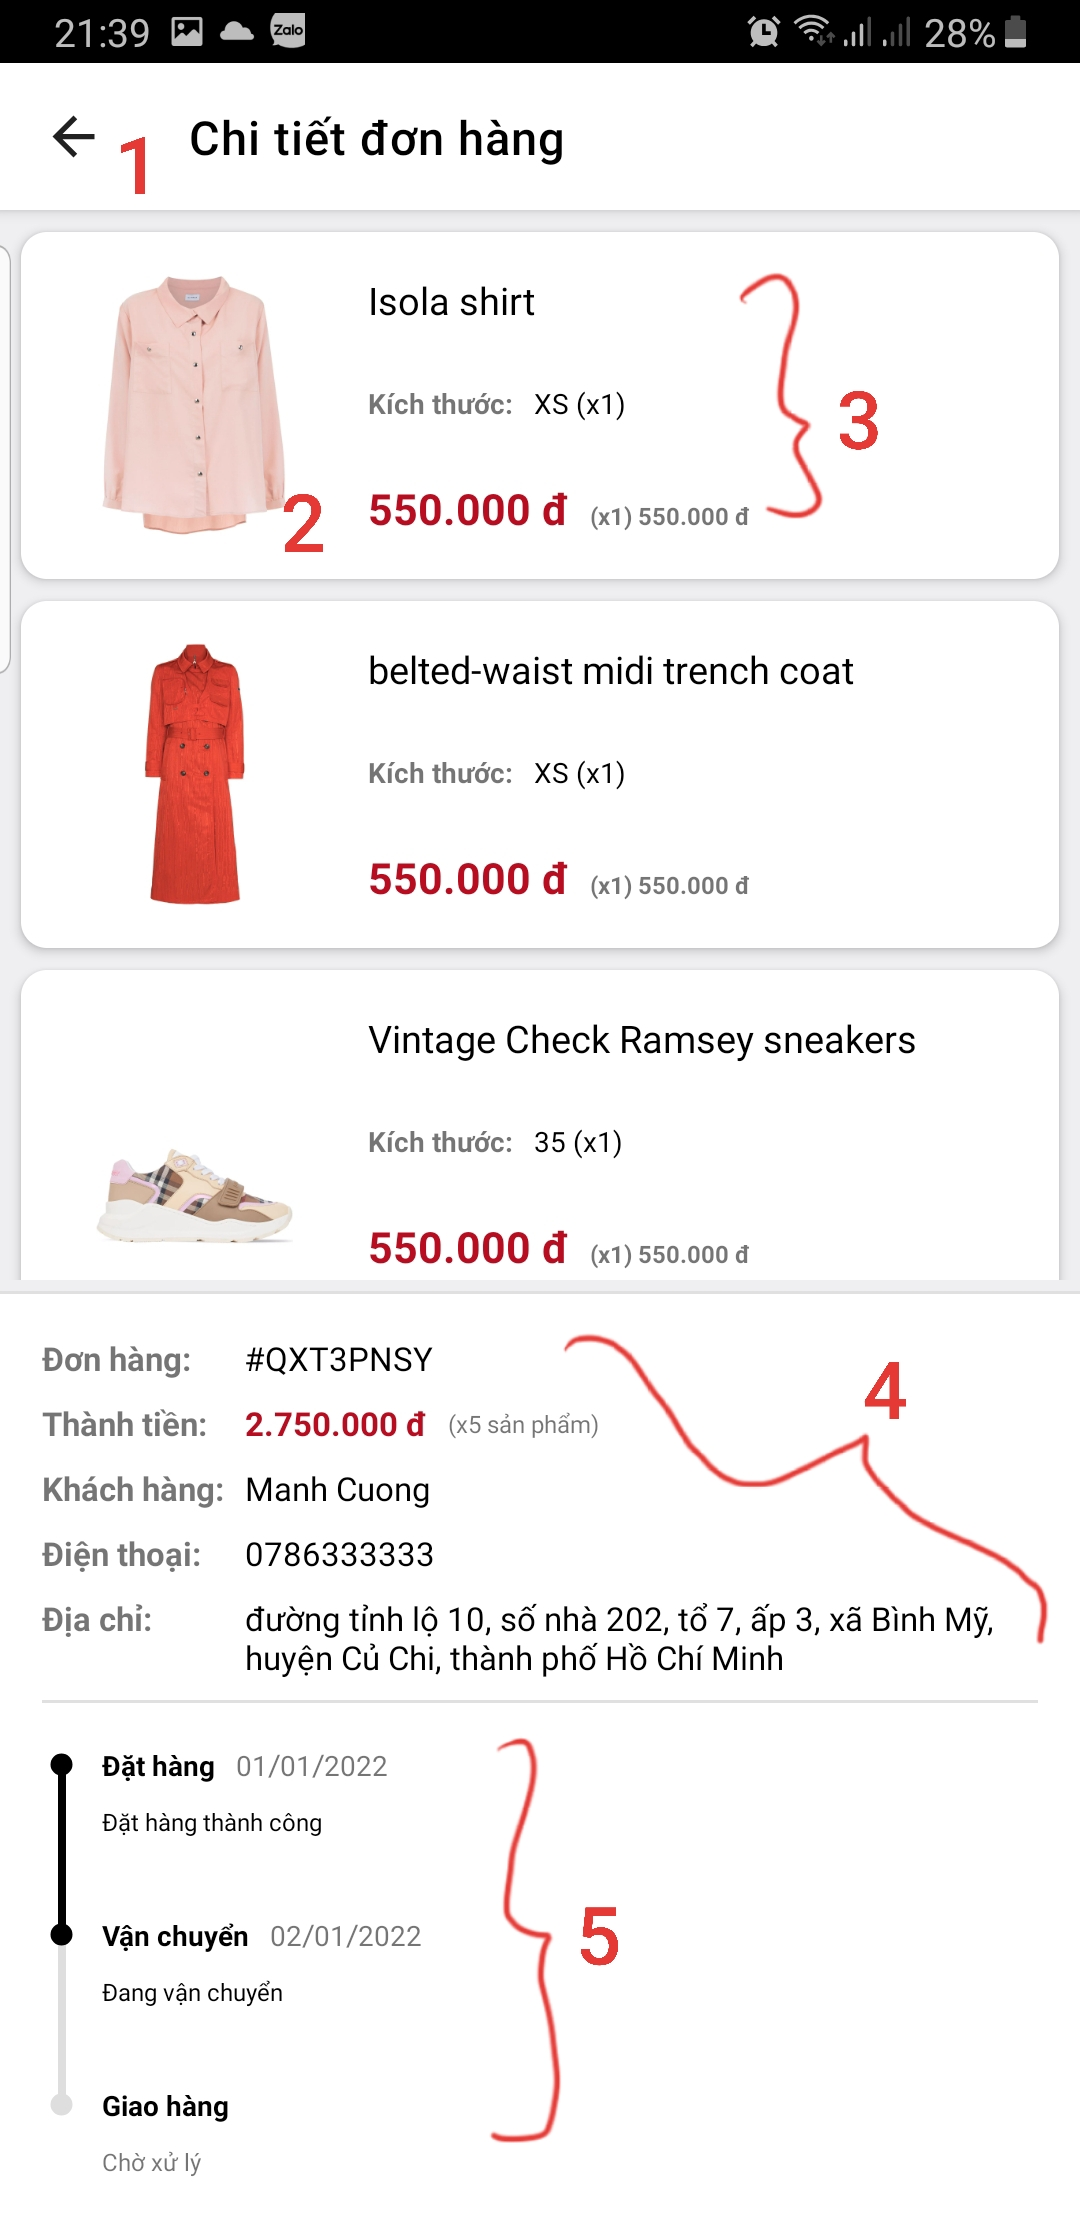
\includegraphics[height=10cm]{images/37.png}
    \caption{Màn hình chi tiết đơn hàng}
\end{figure}

\indent \textbf{Các thành phần và chức năng kèm theo trên màn hình}
\begin{itemize}
    \item \textbf{1}: As home indicator - dùng để quay lại màn hình lịch sử đơn hàng.
    \item \textbf{2}: Image View - hiển thị hình ảnh của một sản phẩm trong đơn hàng, khi nhấn vào người dùng sẽ được đưa đến trang chi tiết sản phẩm.
    \item \textbf{3}: Các Text view - thể hiện các thông tin về sản phẩm bao gồm tên sản phẩm, kích thước + số lượng, tổng tiền cho sản phẩm này.
    \item \textbf{4}: Các Text view - thể hiện các thông tin chi tiết cho toàn bộ đơn hàng này.
    \item \textbf{5}: Hiển thị trạng thái hiện tại của đơn hàng.
\end{itemize}

\subsubsection{Màn hình tài khoản người dùng}
Được thực hiện bởi sinh viên 19424015.\\

\indent Màn hình này thể hiện chi tiết của một đơn hàng, được truy cập khi người dùng nhấn vào một item của Vertical Recycler View ở màn hình lịch sử đơn hàng ở mục 2.3.9. Dưới đây là hình chụp của màn hình này.

\begin{figure}[H]
    \centering
    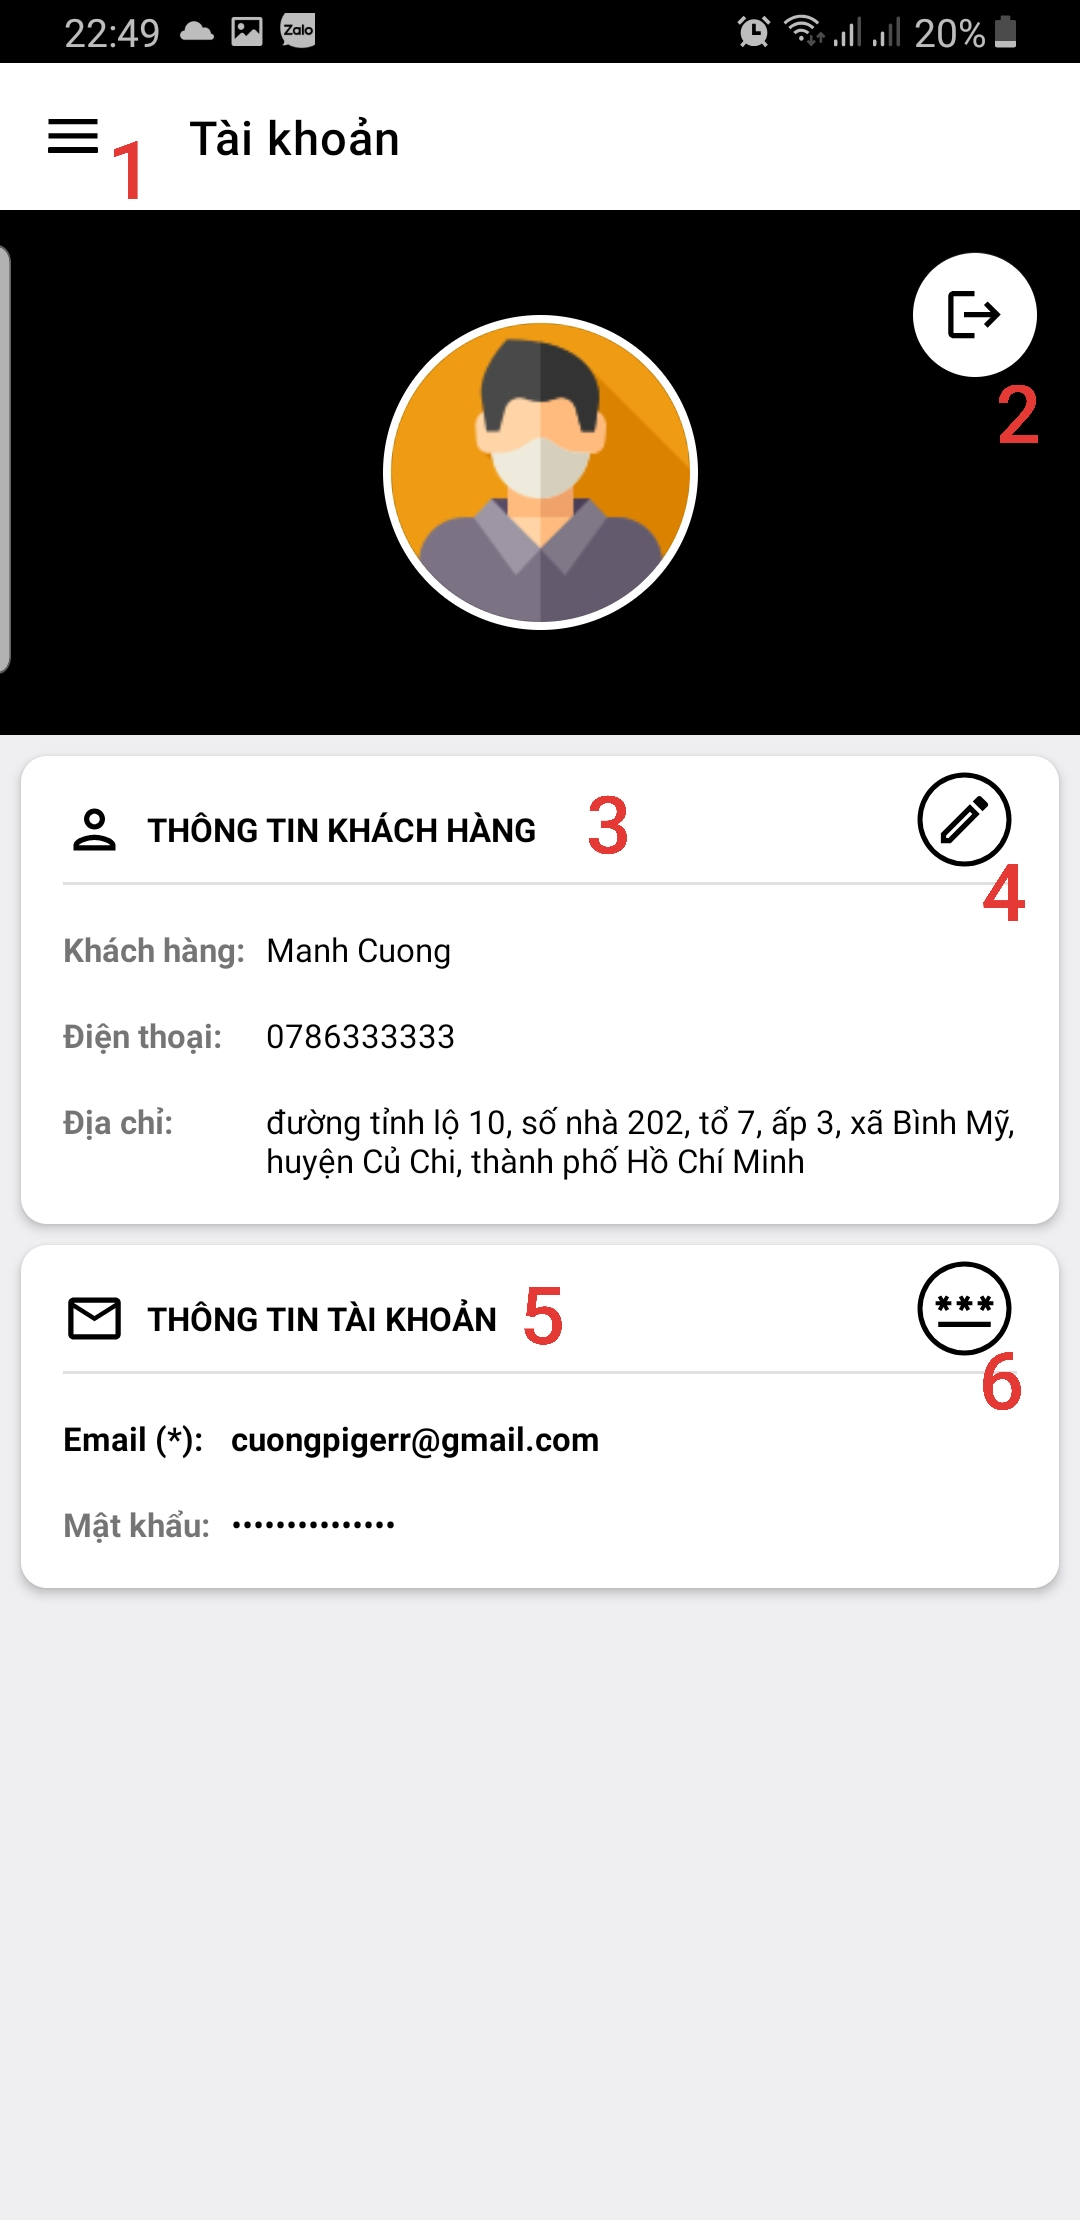
\includegraphics[height=10cm]{images/38.png}
    \caption{Màn hình tài khoản người dùng}
\end{figure}

\begin{figure}[H]
    \centering
    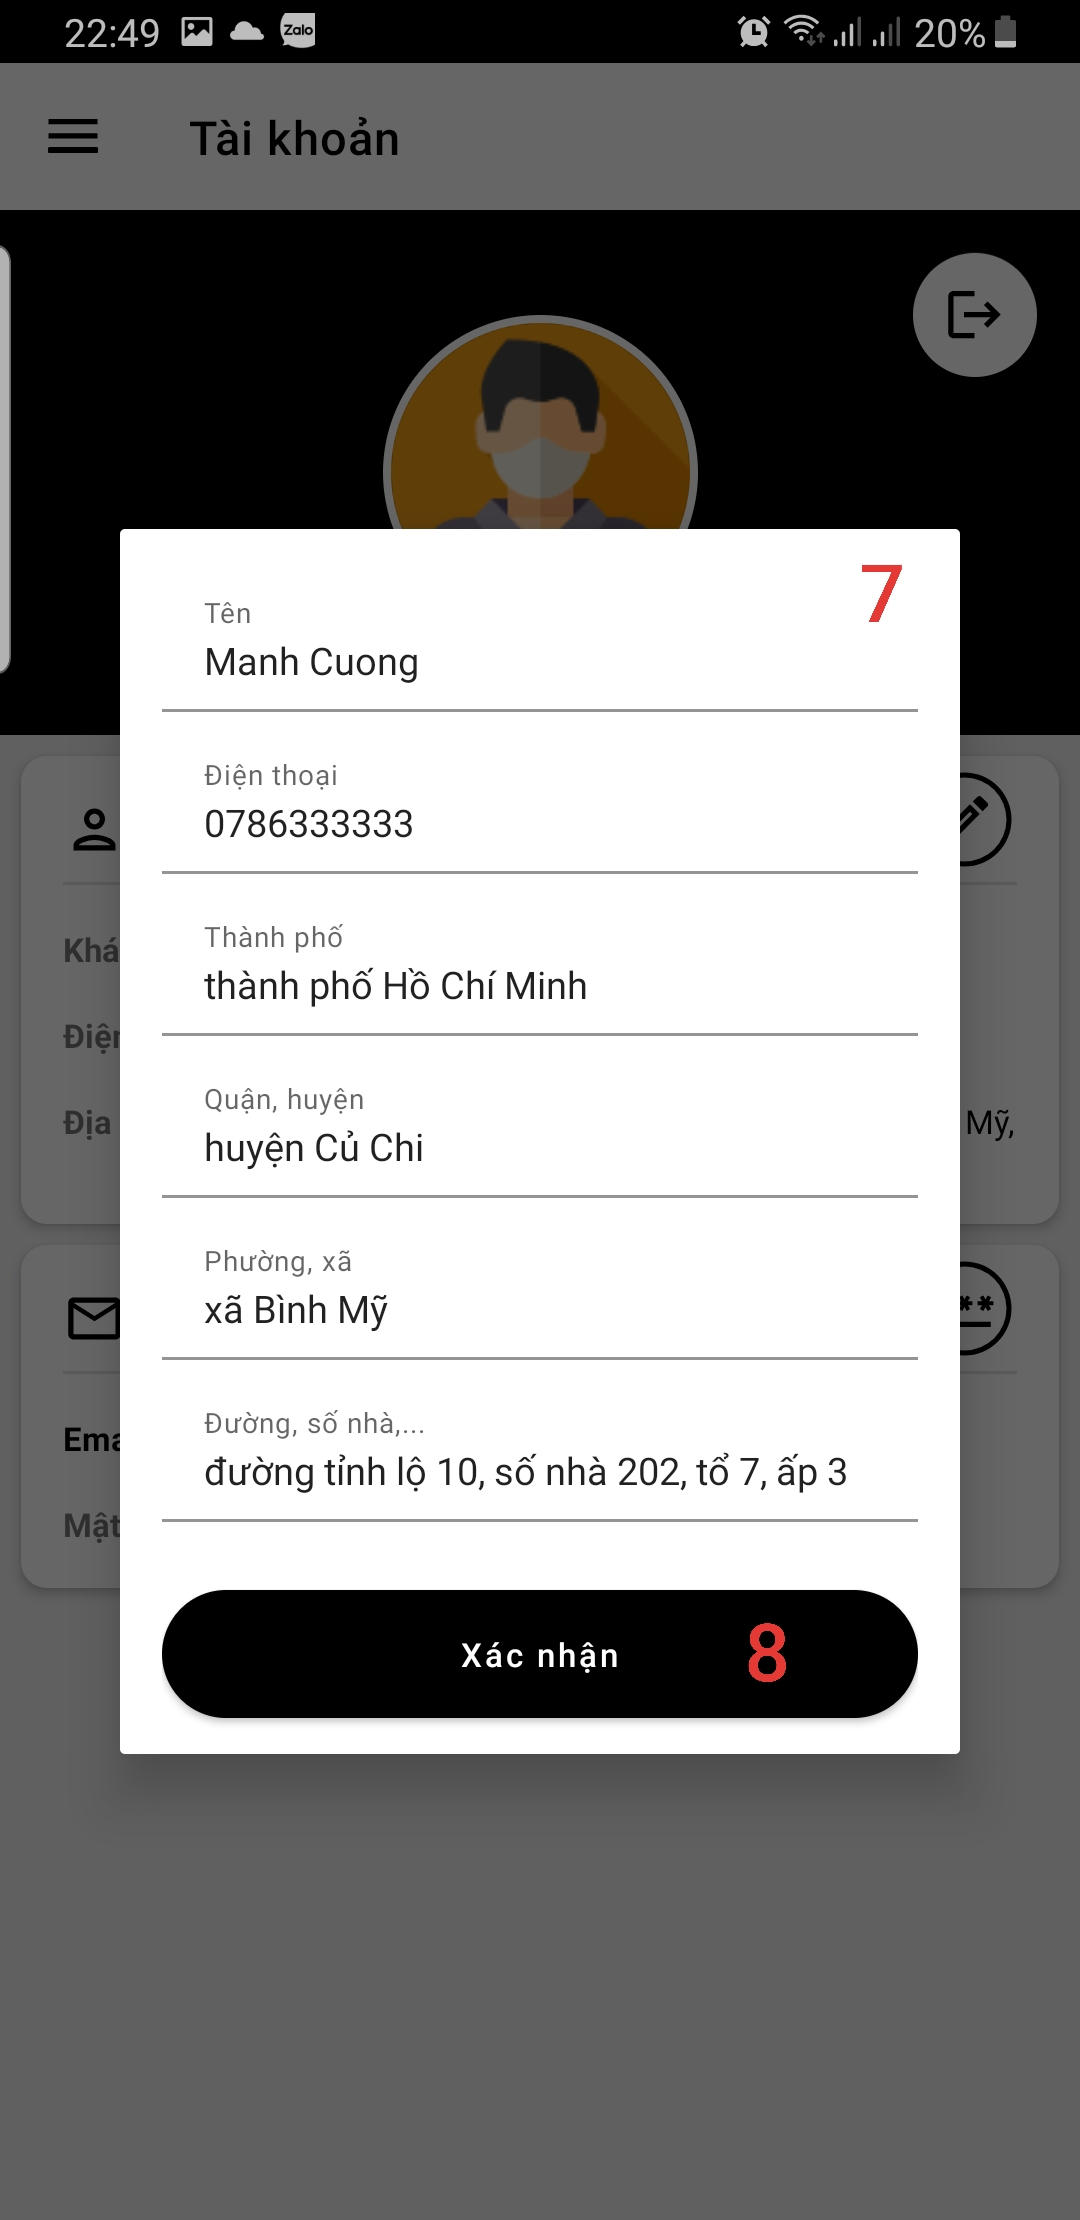
\includegraphics[height=10cm]{images/39.png}
    \caption{Màn hình tài khoản người dùng - chỉnh sửa địa chỉ giao hàng mặc định}
\end{figure}

\begin{figure}[H]
    \centering
    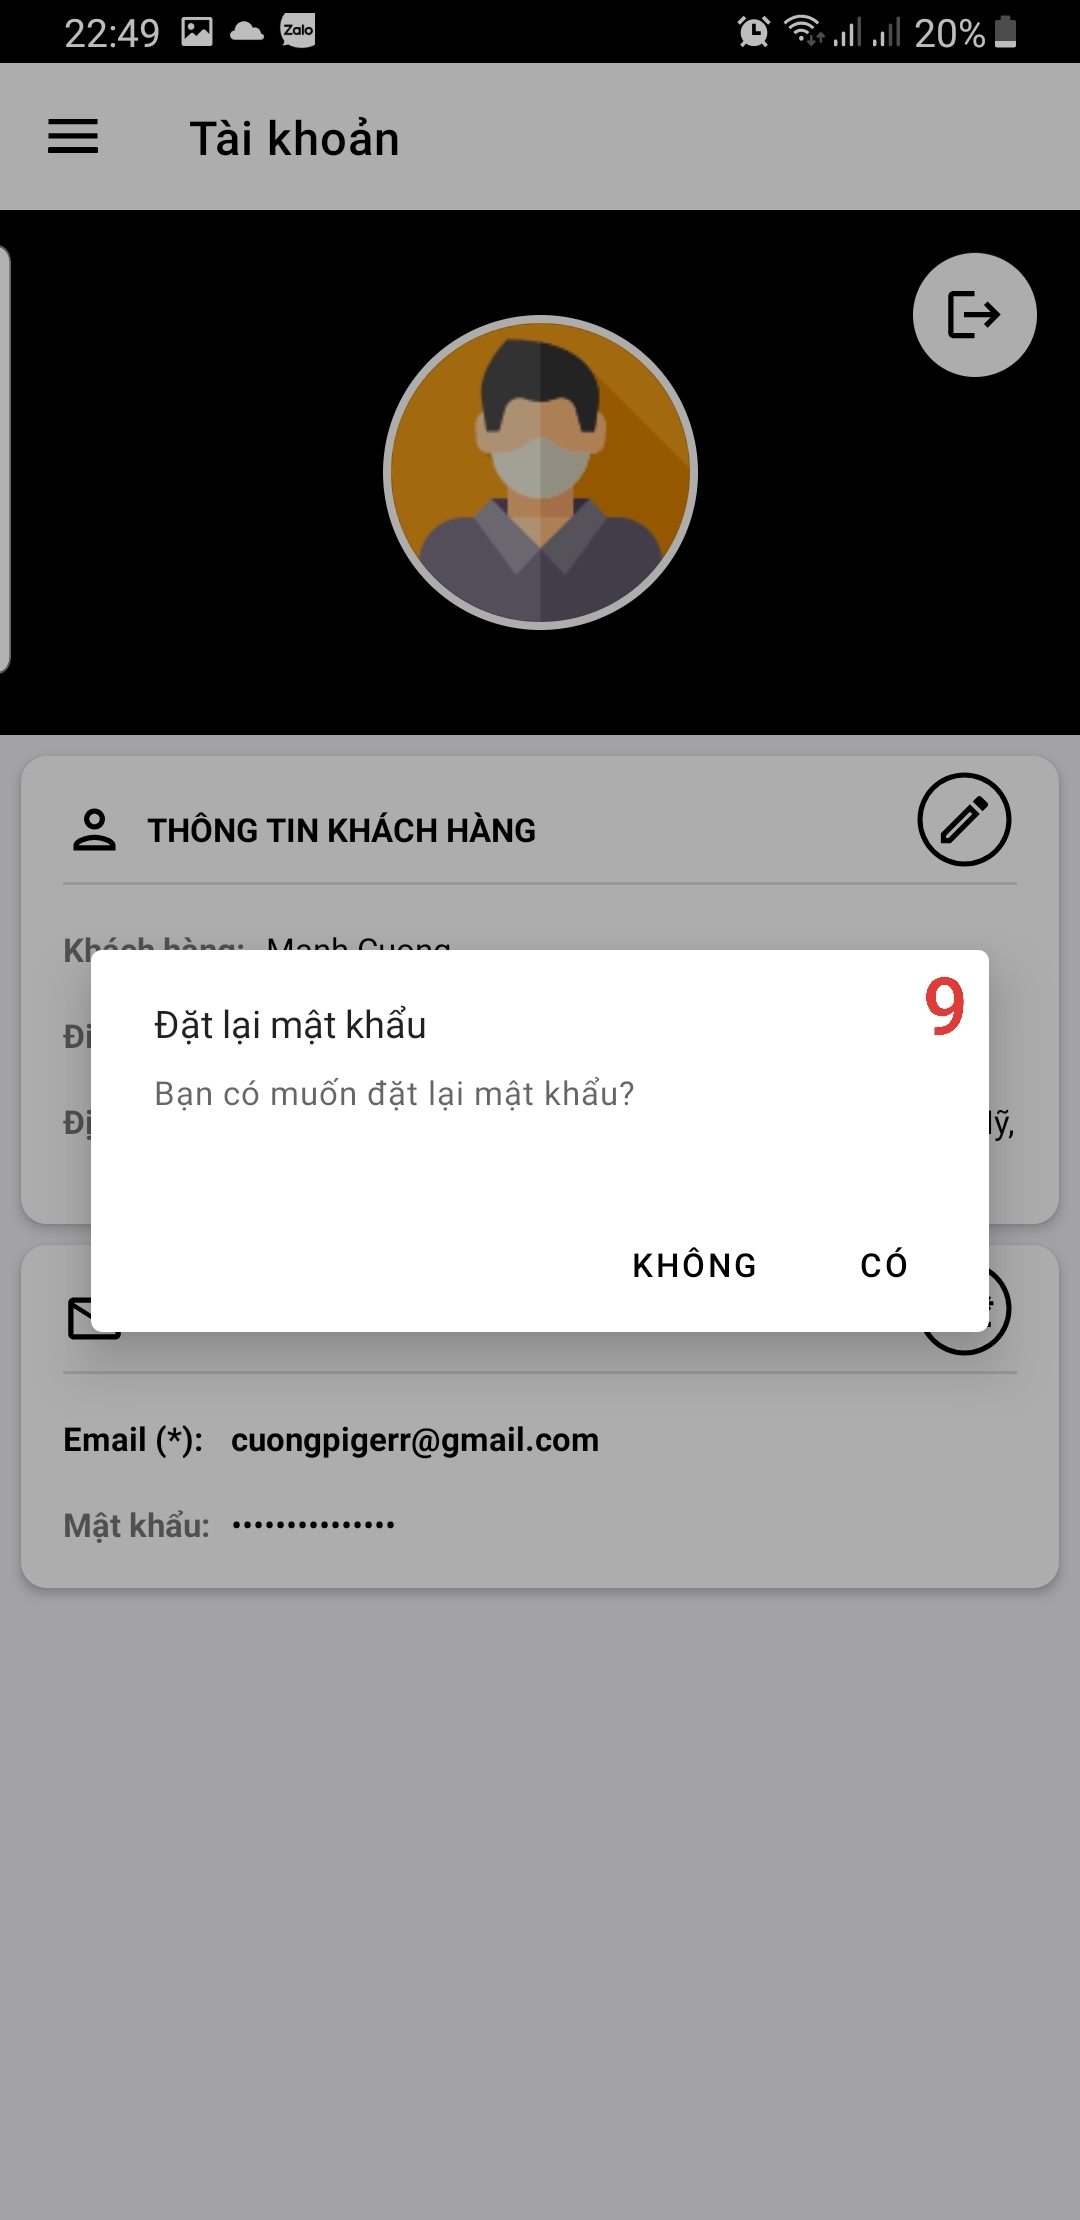
\includegraphics[height=10cm]{images/40.png}
    \caption{Màn hình tài khoản người dùng - đặt lại mật khẩu}
\end{figure}

\begin{figure}[H]
    \centering
    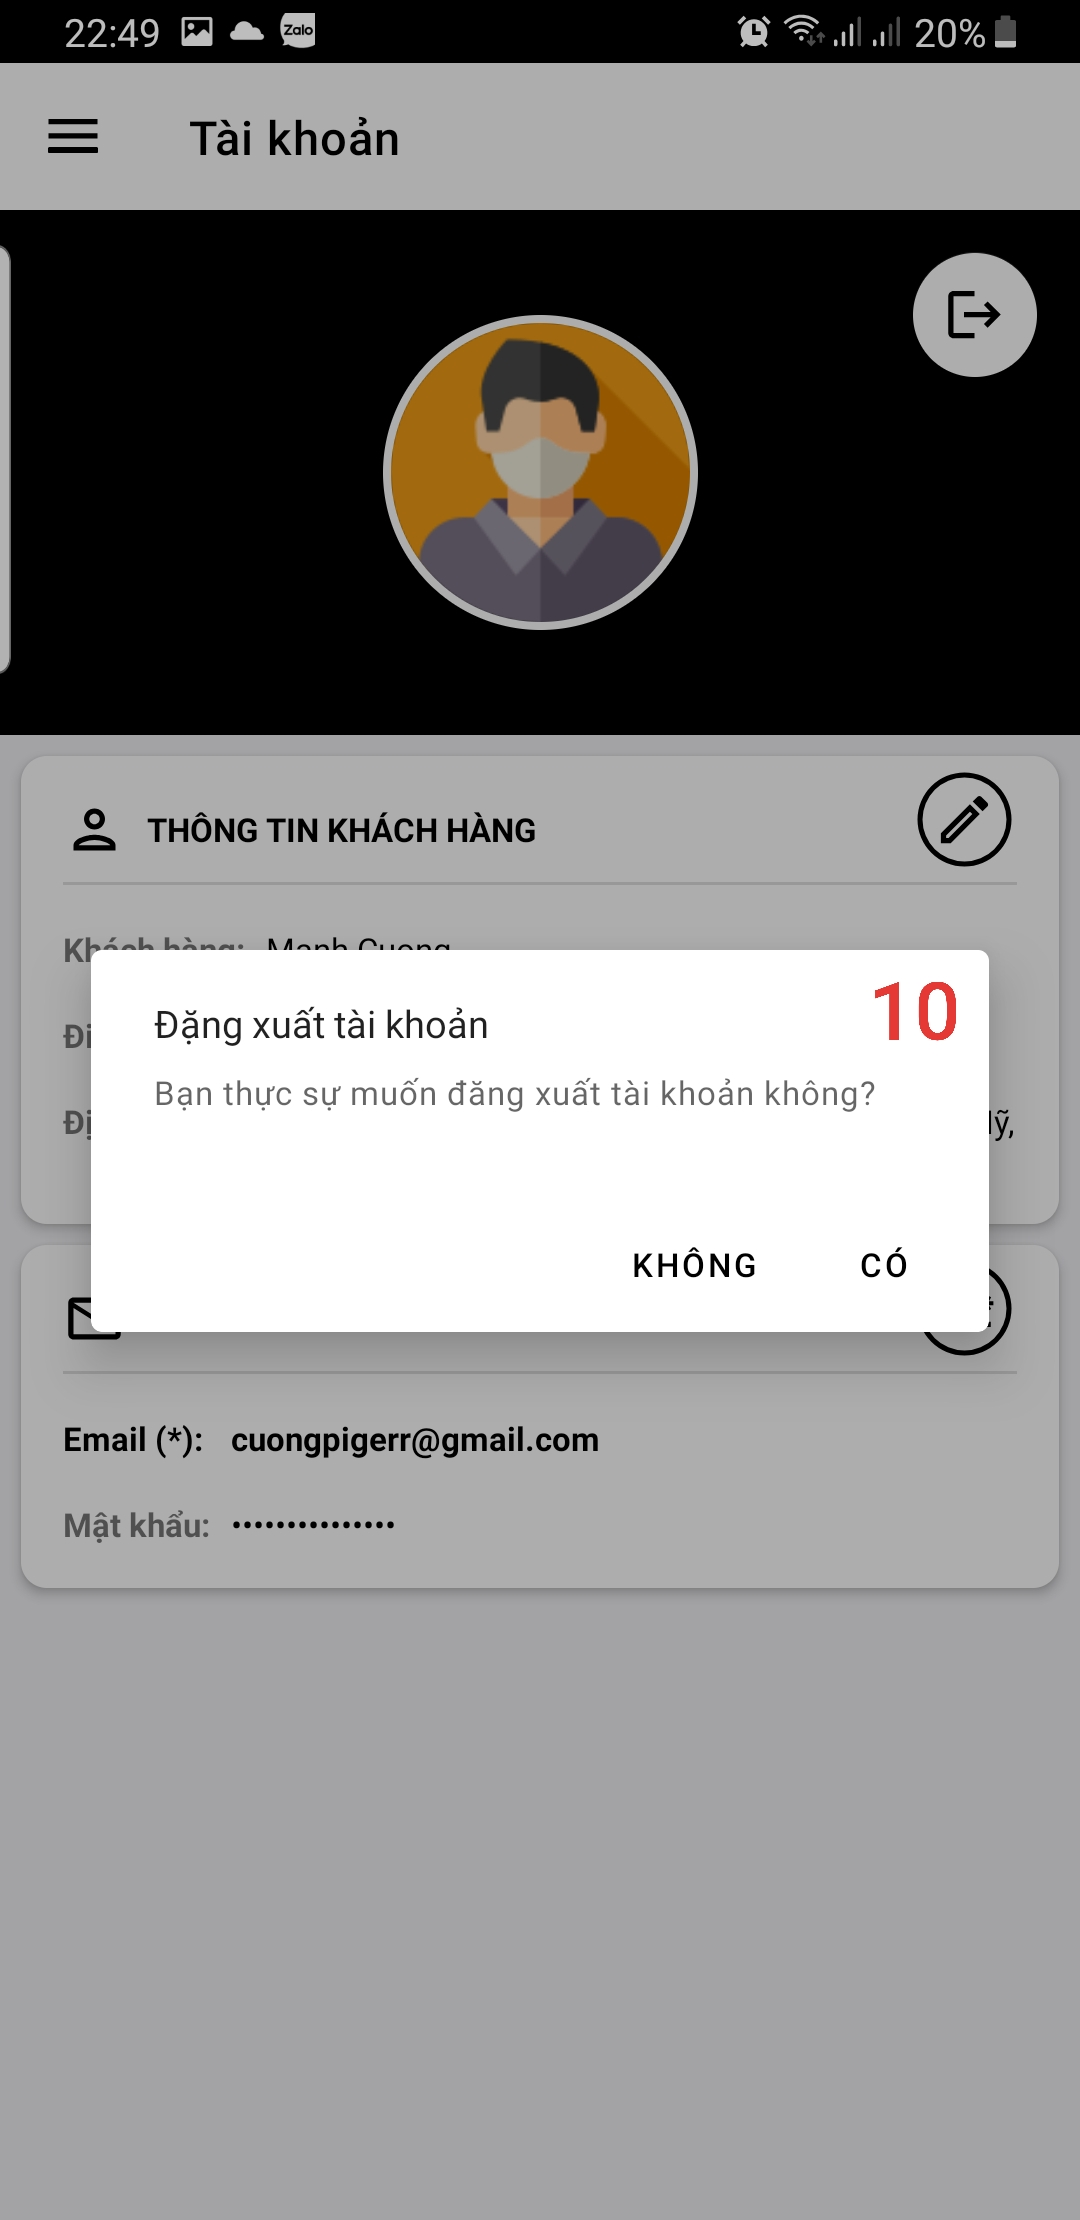
\includegraphics[height=10cm]{images/41.png}
    \caption{Màn hình tài khoản người dùng - đăng xuất}
\end{figure}

\indent \textbf{Các thành phần và chức năng kèm theo trên màn hình}
\begin{itemize}
    \item \textbf{1}: Hamburger toggle - dùng để truy cập vào navigation view.
    \item \textbf{2}: Floating action button - khi người dùng nhấn vào sẽ hiện lên một alert dialog để hỏi lại người dùng có muốn đăng xuất hay không. 
    \item \textbf{3}: Các text view - thể hiện các thông tin về địa chỉ giao hàng mặc định của người dùng.
    \item \textbf{4}: Image button - nhấn vào sẽ hiện một dialog để người dùng cập nhật địa chỉ giao hàng mặc định.
    \item \textbf{5}: Các text view - cho biết email của người dùng (không thể thay đổi email).
    \item \textbf{6}: Image button - nhấn vào một alert dialog hiện lên hỏi người dùng có muốn đặt lại password không.
    \item \textbf{7}: Dialog - hiển thị các Text input layout để người dùng cập nhật địa chỉ giao hàng mặc định, dialog này hiện lên khi người dùng nhấn vào thành phần \textbf{4}.
    \item \textbf{8}: Button - khi người dùng nhấn vào thì địa chỉ giao hàng mặc định sẽ được cập nhật dựa vào những thông tin mà người dùng vừa nhập vào dialog.
    \item \textbf{9}: Alert dialog - hiển thị ra khi người dùng nhấn vào thành phần \textbf{6}, nếu người dùng chọn "Có" thì một mail đặt lại mật khẩu được gửi về email mà người dùng dùng đăng ký tài khoản.
    \item \textbf{10}: Alert dialog - hiển thị ra khi người dùng nhấn vào thành phần \textbf{2} để xác nhận người dùng có muốn đăng xuất không, nếu người dùng chọn có thì ứng dụng sẽ đăng xuất tài khoản và quay về trang Splash Screen.
\end{itemize}

\section{Những điểm đặc biệt trong đồ án}
\subsection{Về giao diện}
Nhóm tìm hiểu về phong cách thiết kế Material Design trên trang \url{https://material.io}

\subsection{Về kho lưu trữ, CSDL và Authentication}
Nhòm tìm hiểu về các dịch vụ lưu trự Firestore, dịch vụ lưu trự file Firestorage và xác thực Authentication được cung cấp từ Google.

\subsection{Chức năng tìm kiếm}
Vì chức năng tìm kiếm này dựa theo tên của sản phẩm, trong Firestore có một phương thức là \texttt{whereArrayContainsAny()} để xem một trường dạng mảng trong document có chứa giá trị nào phù hợp trong mảng đầu vào không. Nến nhóm lợi dụng phương thức này để thực hiện chức năng tìm kiếm, dưới đây là cách nhóm tổ chức các trường dữ liệu của sản phẩm được lưu trữ trong CSDL.

\begin{figure}[H]
    \centering
    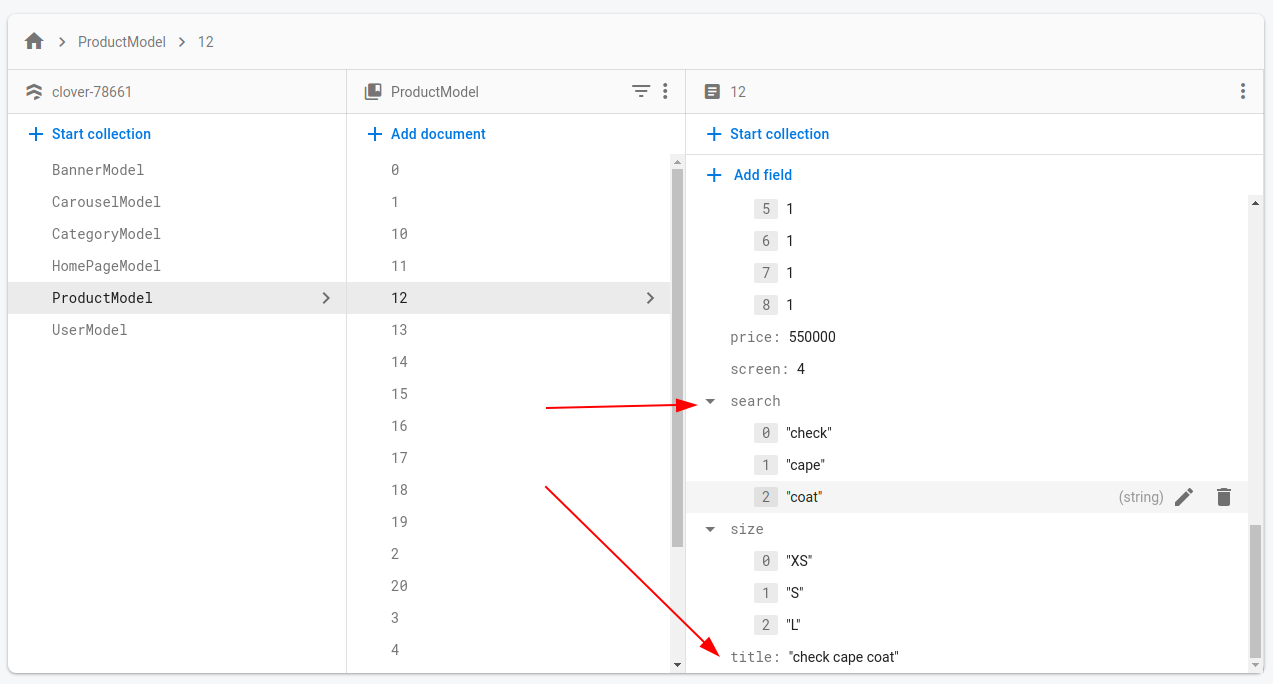
\includegraphics[width=\textwidth]{images/42.png}
    \caption{ProductModel - được lưu trữ trong Firestore}
\end{figure}

\indent ở đây trường \texttt{search} chính là trường \texttt{title} được nhóm lưu dưới dạng mảng để thực hiện chức năng tìm kiếm.

\section{Tham khảo}
\begin{itemize}
    \item Logo ứng dụng và tên Clover: được nhóm xin phép từ nhãn hàng Clover và đã được sự đồng ý từ chị chủ nhãn hàng, trang bán hàng của shop tại \url{https://www.facebook.com/TiemmaynhaAn}.
    \item Về hình ảnh người mẫu Việt Nam ở mục sản phẩm mới: là bạn Phan Hữu Lộc - cựu sinh viên K17 khoa Sinh học của trường Đại Học Khoa Học Tự Nhiên TP.HCM và là người mẫu của nhãn hàng Clover phía trên.
    \item Các hình ảnh sản phẩm khác được nhóm lấy về (chưa xin phép) từ trang bán hàng Farfetch tại \url{https://www.farfetch.com}. Và do nhóm đã lấy về cách đây khá lâu nên đường link chi tiết của từng sản phẩm nhóm không nắm rõ được nữa, nhóm xin gửi lời xin lỗi đến Thầy vì sự cố này của nhóm.
    \item Về các kĩ thuật code trong đồ án ngoài slide của Thầy lý thuyết nhóm còn tham khảo thêm trong cuốn \textbf{Android Programming for Beginners}, link sách tại \url{https://www.amazon.com/Android-Programming-Beginners-depth-full-featured/dp/1800563434}.
\end{itemize}


\end{document}